
\documentclass[a4paper]{article}

\usepackage[english]{babel}
\usepackage[utf8]{inputenc}

\usepackage[utf8]{vietnam}
\usepackage{a4wide,amssymb,epsfig,latexsym,array,hhline,fancyhdr}
\usepackage[normalem]{ulem}
\usepackage{soul}
\usepackage{listings}

\usepackage[makeroom]{cancel}
\usepackage{amsmath}
\usepackage{amsthm}
\usepackage{multicol,longtable,amscd}
\usepackage{diagbox}%Make diagonal lines in tables
\usepackage{booktabs}
\usepackage{alltt}
\usepackage[framemethod=tikz]{mdframed}% For highlighting paragraph backgrounds
\usepackage{caption,subcaption}
\usepackage{float}

\usepackage{lastpage}
\usepackage[lined,boxed,commentsnumbered]{algorithm2e}
\usepackage{enumerate}
\usepackage{color}
\usepackage{graphicx}							% Standard graphics package
\usepackage{array}
\usepackage{tabularx, caption}
\usepackage{multirow}
\usepackage{multicol}
\usepackage{rotating}
\usepackage{graphics}
\usepackage{geometry}
\usepackage{setspace}
\usepackage{epsfig}
\usepackage{tikz}
\usetikzlibrary{arrows,backgrounds}
\usepackage[unicode]{hyperref}
\hypersetup{urlcolor=blue,linkcolor=black,citecolor=black,colorlinks=true} 
\usepackage{pstricks} 								% PSTricks with the standard color package

\usepackage[normalem]{ulem}

\newtheorem{theorem}{{\bf Định lý}}
\newtheorem{property}{{\bf Tính chất}}
\newtheorem{proposition}{{\bf Mệnh đề}}
\newtheorem{corollary}[proposition]{{\bf Hệ quả}}
\newtheorem{lemma}[proposition]{{\bf Bổ đề}}
\theoremstyle{definition}
\newtheorem{exer}{Bài toán}

\def\thesislayout{	% A4: 210 × 297
	\geometry{
		a4paper,
		total={160mm,240mm},  % fix over page
		left=30mm,
		top=30mm,
	}
}
\thesislayout

\usepackage{fancyhdr}
\setlength{\headheight}{40pt}
\pagestyle{fancy}
\fancyhead{} % clear all header fields
\fancyhead[L]{
	\begin{tabular}{rl}
		\begin{picture}(25,15)(0,0)
			\put(0,-8){
\includegraphics[width=8mm, height=8mm]{Images/hcmut.png}}
			%\put(0,-8){\epsfig{width=10mm,figure=hcmut.eps}}
		\end{picture}&
		%
\includegraphics[width=8mm, height=8mm]{Images/hcmut.png} & %
		\begin{tabular}{l}
			\textbf{\bf \ttfamily Trường Đại Học Bách Khoa Tp.Hồ Chí Minh}\\
			\textbf{\bf \ttfamily Khoa Khoa Học \& Kỹ Thuật Máy Tính}
		\end{tabular} 	
	\end{tabular}
}
\fancyhead[R]{
	\begin{tabular}{l}
		\tiny \bf \\
		\tiny \bf 
\end{tabular}  }
\fancyfoot{} % clear all footer fields
\fancyfoot[L]{\scriptsize \ttfamily Đề bài tập lớn môn Cấu trúc Rời rạc cho KHMT (CO1007) - Niên khóa 2019-2020}
\fancyfoot[R]{\scriptsize \ttfamily Trang {\thepage}/\pageref{LastPage}}
\renewcommand{\headrulewidth}{0.3pt}
\renewcommand{\footrulewidth}{0.3pt}


%%%
\setcounter{secnumdepth}{4}
\setcounter{tocdepth}{3}
\makeatletter
\newcounter {subsubsubsection}[subsubsection]
\renewcommand\thesubsubsubsection{\thesubsubsection .\@alph\c@subsubsubsection}
\newcommand\subsubsubsection{\@startsection{subsubsubsection}{4}{\z@}%
	{-3.25ex\@plus -1ex \@minus -.2ex}%
	{1.5ex \@plus .2ex}%
	{\normalfont\normalsize\bfseries}}
\newcommand*\l@subsubsubsection{\@dottedtocline{3}{10.0em}{4.1em}}
\newcommand*{\subsubsubsectionmark}[1]{}
\makeatother

\everymath{\color{blue}}%make in-line maths symbols blue to read/check easily

\sloppy
\captionsetup[figure]{labelfont={small,bf},textfont={small,it},belowskip=-1pt,aboveskip=-9pt}
%space remove between caption, figure, and text
\captionsetup[table]{labelfont={small,bf},textfont={small,it},belowskip=-1pt,aboveskip=7pt}
%space remove between caption, table, and text

%\floatplacement{figure}{H}%forced here float placement automatically for figures
%\floatplacement{table}{H}%forced here float placement automatically for table
%the following settings (11 lines) are to remove white space before or after the figures and tables
%\setcounter{topnumber}{2}
%\setcounter{bottomnumber}{2}
%\setcounter{totalnumber}{4}
%\renewcommand{\topfraction}{0.85}
%\renewcommand{\bottomfraction}{0.85}
%\renewcommand{\textfraction}{0.15}
%\renewcommand{\floatpagefraction}{0.8}
%\renewcommand{\textfraction}{0.1}
\setlength{\floatsep}{5pt plus 2pt minus 2pt}
\setlength{\textfloatsep}{5pt plus 2pt minus 2pt}
\setlength{\intextsep}{10pt plus 2pt minus 2pt}

\thesislayout

\begin{document}
	\lstset{
		language=R,
	    backgroundcolor=\color{lightgray},
	    title=Source code,
	    keywordstyle=\color{black},
	    frame=single
	}
	
	\begin{titlepage}
		\begin{center}
			ĐẠI HỌC QUỐC GIA THÀNH PHỐ HỒ CHÍ MINH \\
			TRƯỜNG ĐẠI HỌC BÁCH KHOA \\
			KHOA KHOA HỌC \& KỸ THUẬT MÁY TÍNH 
		\end{center}
		
		\vspace{1cm}
		
		\begin{figure}[h!]
			\begin{center}
				
\includegraphics[width=3cm]{Images/hcmut.png}
			\end{center}
		\end{figure}
		
		\vspace{1cm}
		
		
		\begin{center}
			\begin{tabular}{c}
				\multicolumn{1}{l}{\textbf{{\Large CẤU TRÚC RỜI RẠC CHO KHMT (CO1007)}}}\\
				~~\\
				\hline
				\\
				% \multicolumn{1}{l}{\textbf{{\Large Đề bài tập lớn cho Nhóm $n$}}}\\
				% \\
				% \textbf{{\Huge Thống kê mô tả và}} \\
				% \textbf{{\Huge Xác suất rời rạc với R}}\\
				\textbf{\large Thống kê khảo sát kết quả Covid-19}\\
				\textbf{\large môn Cấu trúc rời rạc}
				\\
				\hline
			\end{tabular}
		\end{center}
		
		\vspace{1.5cm}
		
		\begin{table}[h]
			\begin{tabular}{rrl}
				\hspace{5 cm} & GVHD: & Huỳnh Tường Nguyên\\
				\hspace{5 cm} &  & Nguyễn Ngọc Lễ\\
				
				& SV thực hiện: & Lê Nhật Anh -- 2153158 \\
				& & Kim Gia Bảo -- 2152417 \\
				& & Đỗ Nhật Thái -- 2152964 \\
				& & Nguyễn Thế Cường -- 2153240 \\
			\end{tabular}
		\end{table}
		\vspace{1.5cm}
		\begin{center}
			{\footnotesize Tp. Hồ Chí Minh, Tháng 04/2022}
		\end{center}
	\end{titlepage}

\newpage
\tableofcontents
\newpage


\section{Động cơ nghiên cứu}\label{motivation}
$\indent$Bệnh Corona do virus gây ra còn gọi là COVID-19 đã tạo ra những tác động tiêu cực đến nền đời sống của cư dân trên thề giới. Các đợt bùng phát của COVID-19 hay những biến thể virus đã mang đến những thách thức chưa từng có và được dự báo sẽ có tác động đáng kể đến sự phát triển kinh tế. Nhiều thông tin, tin tức về tình hình dịch bệnh cũng như dữ liệu về COVID-19 được phổ biến rộng rải trong đời sống hay trên internet để giúp cho mọi người quan sát, phân tích, nghiên cứu đươc cập nhật hàng ngày.

Phân tích \& thống kê dữ liệu về COVID-19 giúp cho ta thấy được số ca nhiễm bệnh, tử vong của một quốc gia, so sánh tình trạng của các quốc gia trong khu vực hay diễn biến dịch trên thế giới. Từ số liệu được báo cáo mơi chúng ta muốn biết các ca nhiễm bệnh có xu hướng tăng lên hay giảm xuống quy mô các đợt bùng phát ở mỗi quốc gia. Dữ liệu dùng cho bài tập lớn có tham khào từ \url{https://github.com/owid/covid-19-data/blob/master/public/data/README.md} {nguồn} có thể xử lý trước với một vài thống kê cơ bản trước khi nó được truyền đi để khai thác dữ liệu thông minh sâu hơn. 


\section{Mục tiêu}\label{objective}
$\indent$  
Trong bài tập lớn này, các sinh viên sẽ bắt đầu với các bài toán thống kê đơn giản từ những dữ liệu được cung cấp. Qua đó, các em sẽ tìm ra những con số thú vị, có ý nghĩa đối với các dữ liệu thực tế từ tình hình dịch corona. Những kết quả mà các em tìm ra sẽ là bước khởi đầu cho việc khai phá nguồn dữ liệu của hệ thống sau này, nhằm đạt tới mục tiêu nâng cao kỹ năng lập trình, kỹ năng giải quyết vấn đề cho người học, kỹ năng làm việc nhóm cũng như hướng tới mục tiêu cao hơn là đam mê trong làm việc, học tập và nghiên cứu.

\section{Cơ sở lý thuyết}\label{theory}
\subsection{ Bách phân vị và tứ phân vị}
\subsubsection{Định nghĩa}
\begin{itemize}
    \item Bách phân vị (Percentile) là đại lượng dùng để ước tính tỷ lệ dữ liệu trong một tập số liệu rơi vào vùng cao hơn hoặc thấp hơn so với một giá trị cho trước. Bách phân vị chia dữ liệu có thứ tự theo hàng trăm.
    \item Tứ phân vị (Quartile) là một trường hợp đặc biệt của bách phân vị. Tứ phân vị có 3 giá trị, đó là tứ phân vị thứ nhất, thứ nhì, và thứ ba. Ba giá trị này chia một tập hợp dữ liệu đã sắp xếp theo thứ tự thành 4 phần có số lượng quan sát đều nhau.
\end{itemize}
\subsubsection{Công thức}
\begin{enumerate}[a)]
    
 \item Xác định giá trị bách phân vị\\
Để xác định giá trị (vp) của phân vị thứ p trong một tập dữ liệu, ta thực hiện theo các bước sau:
\begin{itemize}
    \item Sắp xếp dữ liệu theo thứ tự từ nhỏ nhất đến lớn nhất.
    \item Tính chỉ số i
    $$
i=\frac{p \times(n+1)}{100}
$$
\end{itemize}
Trong đó:
\begin{itemize}
    \item $i$ là vị trí của giá trị dữ liệu tại phân vị thứ p
    \item $p$ là phân vị thứ p
    \item $n$ là tổng số quan sát
\end{itemize}
 \item Xác định giá trị tứ phân vị:
\begin{itemize}
    \item Giá trị tứ phân vị thứ nhất Q1 bằng trung vị phần dưới, tương đương với bách phân vị thứ 25.
    \item Giá trị tứ phân vị thứ hai Q2 chính bằng giá trị trung vị, tương đương với bách phân vị thứ 50.
    \item Giá trị tứ phân vị thứ ba Q3 bằng trung vị phần trên, tương đương với bách phân vị thứ 75.
\end{itemize}
\end{enumerate}
\subsection{Giá trị trung bình}
\subsubsection{Định nghĩa}
$\indent$   Giá trị trung bình là một loại trung bình được tính bằng cách chia tổng của một tập hợp số cho số lượng các số trong tập hợp đó.
\subsubsection{Công thức}
$$\bar{a} = \frac{(a_1+a_2+\ldots+a_n)}{n}= \frac{(\sum\of a)}{n}$$
Trong đó:
\begin{itemize}
    \item 	$\bar{a}$ là giá trị trung bình
    \item 	$a_1, a_2,\ldot, a_n$ là các số trong tập hợp
    \item 	$n$ là số các số lượng các số trong tập hợp
\end{itemize}
\subsection{Độ lệch chuẩn}
\subsubsection{Định nghĩa}
$\indent$ Độ lệch chuẩn (Standard deviation) là thước đo độ phân tán của các giá trị trong một tập dữ liệu đã cho từ giá trị trung bình của chúng. Nó cho biết trung bình mỗi giá trị nằm bao xa so với giá trị trung bình.\\
\subsubsection{Công thức}
a) Đối với dữ liệu là một tổng thể:
$$
\sigma=\sqrt{\sigma^{2}}=\sqrt{\frac{1}{N} \sum_{i=1}^{N}\left(x_{i}-\mu\right)^{2}}
$$
Trong đó: 
\begin{itemize}
    \item $x_{i}$ là giá trị của quan sát thứ i
    \item $\mu$ là giá trị trung bình tổng thể
    \item $N$ là tổng số quan sát của tổng thể
\end{itemize}
b) Đối với dữ liệu là một mẫu từ tổng thể:
$$
s=\sqrt{s^{2}}=\sqrt{\frac{1}{n-1} \sum_{i=1}^{N}\left(x_{i}-\bar{x}\right)^{2}}
$$
Trong đó: 
\begin{itemize}
    \item $x_{i}$ là giá trị của quan sát thứ i
    \item $\bar{x}$ là giá trị trung bình của mẫu dữ liệu
    \item $n$ là số quan sát trong mẫu dữ liệu
\end{itemize}
\subsection{Dữ liệu ngoại lệ}
\subsubsection{Định nghĩa}
$\indent$ Dữ liệu ngoại lệ (Outliers) là một điểm dữ liệu có sự khác biệt đáng kể so với các quan sát khác. Dữ liệu ngoại lệ có thể xuất hiện do sự thay đổi thang đo hoặc do lỗi từ dữ liệu thu thập (thông thường dữ liệu ngoại lệ dạng này sẽ bị loại khỏi tập dữ liệu). Một giá trị ngoại lệ có thể gây ra vấn đề nghiêm trọng trong quá trình phân tích dữ liệu.
\subsection{Biểu đồ hộp}
\subsubsection{Định nghĩa}
$\indent$ Biểu đồ hộp (Box plot) hay còn gọi là biểu đồ hộp và râu (Box and whisker plot) là biểu đồ diễn tả 5 vị trí phân bố của dữ liệu, đó là: giá trị nhỏ nhất (min), tứ phân vị thứ nhất (Q1), trung vị (median), tứ phân vị thứ 3 (Q3) và giá trị lớn nhất (max).
\subsection{Tần số tích lũy và tần số tích lũy tương đối}
\subsubsection{Định nghĩa}
\begin{itemize}
    \item Các tần số tích lũy là tổng các tần số tuyệt đối f, từ tần số thấp nhất đến tần số thấp nhất tương ứng với một giá trị nào đó của biến. Đổi lại, tần số tuyệt đối là số lần một quan sát xuất hiện trong tập dữ liệu
    \item $AF_{Toi}$ còn được gọi là tần số tích lũy tuyệt đối. Nếu chia cho tổng dữ liệu, chúng ta có tần số tích lũy tương đối, có tổng cuối cùng phải bằng 1.
\end{itemize}
\subsubsection{Công thức}
\begin{itemize}
    \item Tần suất tích lũy của một giá trị nhất định của biến $X_{Toi}$ là tổng các tần số tuyệt đối f của tất cả các giá trị nhỏ hơn hoặc bằng nó:
    $$F_{Toi}  = f_1  + f_2   + f_3    +\ldot+F_{Toi}$$
    \item Tần số tích lũy tương đối: thu được bằng cách chia tần số tích lũy tuyệt đối $f_{Toi}$ cho tổng dữ liệu$N$:
    $$F_r = \frac{f_{Toi}}{N}$$
\end{itemize}


\section{Mô tả dữ liệu}\label{sec:dataset}

$\indent$Dữ liệu gồm các thuộc tính chính  {\bf "iso\_code, continent, location, date, new\_cases,	new\_deaths"} được lưu trong file \textbf{csv}. 
\begin{enumerate}
	\item $iso\_code$: Định danh đất nước 
	\item $continent$ Tên châu lục
	\item $location$: Tên quốc gia
	\item $date$: Ngày quan sát với định dạng Month-Day-Year
	\item $new\_cases$: Số trường hợp COVID-19 mới được xác nhận 
	\item $new\_deaths$: Số tử vong mới do COVID-19 
\end{enumerate}

\section{Nhiệm vụ}\label{requirement} 
Gọi $MD$ là mã đề riêng cho mỗi nhóm (gồm 4 ký số) không trùng nhau, nhóm sinh viên sẽ thực hiện các yêu cầu dưới đây với các giá trị xác định như sau:
$MD = 2179$
\begin{itemize}
	\item  Mỗi nhóm sẽ dùng R để thao tác trên số file dữ liệu khác nhau được chọn theo cột ``STT'' theo cách tính $kq = (kytu1  +  kytu2 +  kytu3 +  kytu4) \% 6$:
	\begin{itemize}
		\item Nếu $kq = 0$ thì làm các stt là {1,2,3}
		\item Nếu $kq = 1$ thì làm các stt là {4,5,6}
		\item Nếu $kq = 2$ thì làm các stt là {7,8,9}
		\item Nếu $kq = 3$ thì làm các stt là {10,11,12} 
		\item Nếu $kq = 4$ thì làm các stt là {13,14,15}
		\item Nếu $kq = 5$ thì làm các stt là {16,17,18}
	\end{itemize}
	
	\item $kq = (2 + 1 + 7 + 9) \% 6 = 1$ làm các stt là {4,5,6}
	
	\begin{center}
		\begin{tabular}{ c | l | c | l}
			
			STT & đất nước & STT & đất nước\\ \hline
			1 & Kenya & 10 & Canada\\ 
			2 & Lesotho &  11 & Greenland\\ 
			3 & Morocco &  12 & United States\\ 
			4 & Indonesia & 13 & Australia \\ 
			5 & Japan  & 14 & New Caledonia\\
			6 & Vietnam  & 15 & New Zealand\\ 
			7 & Andorra  & 16 & Brazil\\ 
			8 & Slovenia  & 17 & Chile\\ 
			9 & United Kingdom & 18 & Venezuela \\
			
			\hline
		\end{tabular}
	\end{center}
\end{itemize}

\begin{enumerate}[i)]
	%i)%
	
	\item \textcolor{orange}{Nhóm câu hỏi liên quan đến tổng quát dữ liệu}\\
	Dùng tập dữ liệu để trả lời các câu hỏi và trình bày theo đinh dạng
	\begin{lstlisting}[frame=single]
library(lubridate)
library(tidyverse)
library(Hmisc)
library(data.table)
library(gridExtra)

#data_input_global_declare
rm(list = ls(all.names = TRUE))
source <- read.csv(file.choose())
data <- source[source[,2]!="",]
data[,5] <- abs(data[,5])
data[,6] <- abs(data[,6])
options("scipen"=10)

world_data <- subset(source, source$location == "World")
iso_code <- c(data$iso_code)
continent <- c(data$continent)
new_cases <- c(data$new_cases)
death_cases <- c(data$new_deaths)
	\end{lstlisting}
\begin{itemize}
    \item Xóa các data từ lần sử dụng trước bằng lệnh $rm(list = ls(all.names = TRUE))$.
    \item Khai báo các thư viện cần thiết.
    \item Tiến hành chọn file dữ liệu và đưa vào biến data.
    \item Loại các dòng không phải đất nước ra khỏi dữ liệu.
\end{itemize}
	\begin{enumerate}[1)]
		
		%%%%%%%i1)%%%%%%
		\item Tập mẫu thể hiện thu thập dữ liệu vào các năm nào
		\begin{lstlisting}[frame=single]  
i1 <- function()
{
date_format <- data
date_format$date <- as.POSIXct(date_format$date , format = "%m/%d/%Y")
outputi1 <- rbind(unique(format(date_format$date, format = "%Y")))
View(outputi1)
}
		\end{lstlisting}
		\begin{itemize}
            \item Đầu tiên ta đưa dữ liệu vào biến data\_format\\
            \item Sau đó ta định dạng lại cột date lại thành kiểu dữ liệu $Date$\\
            \item Sử dụng hàm $unique$ theo format là $\%Y$ để lấy ra các năm theo yêu cầu đề bài.
        \end{itemize}
		\begin{figure}[h!]
		\begin{center}
		    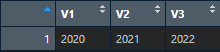
\includegraphics[width=6cm,height=1.5cm]{Images/I/I1.png}
		\end{center}
		\end{figure}
		
		%%%%%i2)%%%%%%%
		\item Số lượng đất nước và định danh của mỗi đất nước (hiển thị 10 đất nước đầu tiên).
		\begin{center}
			\begin{tabular}{ c l }
				iso\_code: & Country \\ 
				AFG & Afghanistan  \\ 
				OWID\_AFR & Africa \\
				ALB & Albania\\ 
				Count & Số đất nước
			\end{tabular}
		\end{center}
		
	\begin{lstlisting}[frame=single]  
i2 <- function()
{
iso_code1 <- unique(data[,1])
location1 <- unique(data[,3])
output_i2 <- rbind(cbind(iso_code1[1:10],location1[1:10]),
                         cbind("Count",length(iso_code1)))
colnames(output_i2) <- c("iso_code","location")
View(output_i2)
}
	\end{lstlisting}
	\begin{itemize}
    \item Ta dùng hàm $unique$ tìm các đất nước và iso\_code chỉ xuất hiện đúng 1 lần trong data gán vào 2 biến. Sau đó ta dùng $rbind$ để tạo data chứa 10 giá trị đầu tiên ở 2 biến iso\_code1 và location1.
\end{itemize}
	\begin{figure}[h!]
		\begin{center}
		    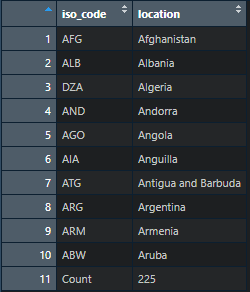
\includegraphics[scale=0.8]{Images/I/I2.png}
		\end{center}
	\end{figure}
	
	%%%%i3)%%%%
		\item Số lượng châu lục trong tập mẫu
		\begin{center}
			\begin{tabular}{ c l }
				Continent : & Số châu lục \\ 
				Africa: & Châu phi \\ 
				Asia: & Châu Á \\
			\end{tabular}
		\end{center}
		\newpage
	\begin{lstlisting}[frame=single]  
i3 <- function()
{
conti <- cbind(unique(data$continent))
conti_trans <- rbind("Chau A","Chau Au",
                      "Chau Phi","Bac Mi",
                      "Nam Mi","Chau Dai Duong")
output_i3 <- data.frame(
conti,
conti_trans
)
output_i3 = rbind(c("Continent",length(conti)),output_i3)
View(output_i3)
}
	\end{lstlisting}
	
	\begin{itemize}
	    \item Ta sử dụng hàm $unique$ để các châu lục chỉ xuất hiện duy nhất 1 lần rồi gán cho biến $conti$, sử dụng hàm $rbind$ để tạo một cột $conti\_trans$ chứa phần phiên dịch tên các châu lục. Cuối cùng ta dùng hàm $length$ để đếm số lượng các phần tử của biến $conti$
	\end{itemize}
	
	\begin{figure}[h!]
		\begin{center}
		    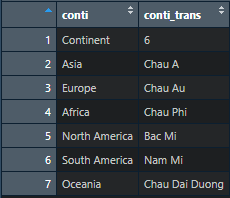
\includegraphics[]{Images/I/I3.png}
		\end{center}
	\end{figure}
	
	
	%%%%%%i4)%%%
		\item Số lượng dữ liệu thể hiện thu thập dữ liệu được trong từng từng châu lục và tổng số
		\begin{center}
			\begin{tabular}{ c l }
				Continent: & Observations \\ 
				Africa & value1  \\ 
				Asia & value2 \\
				Tổng: & giá trị tổng
			\end{tabular}
		\end{center}
		\begin{lstlisting}[frame=single]  
i4 <- function()
{
con_data <- as.numeric(table(data$continent))
con <- sort(unique(data$continent))
sum <- c("Tong:",sum(con_data))
con_data <- data.frame(rbind(cbind(con,con_data),sum))
colnames(con_data) <- c("Continent:", "Observations")
rownames(con_data) <- c(1:nrow(con_data))
View(con_data)
}
	\end{lstlisting}
\begin{itemize}
    \item Ta dùng hàm $table$ để đếm số lần xuất hiện của mỗi châu lục tại cột $Continent$, đây chính là số lượng dữ liệu thu thập đc của mỗi châu lục. Ta biến đổi dữ liệu này thành số và ghép với một cột chứa tên các châu lục tương ứng và tính tổng của chúng rồi ghép vào hàng cuối cùng.
\end{itemize}
	\begin{figure}[h!]
		\begin{center}
		    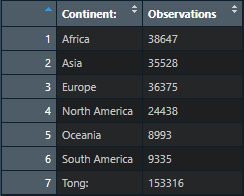
\includegraphics[scale=1.1]{Images/I/I4.png}
		\end{center}
	\end{figure}
		
		%%%%%%i5)%%%%%%%%%%
		\item Số lượng dữ liệu thể hiện thu thập dữ liệu được trong từng từng đất nước (hiển thị 10 dất nước cuối cùng) và tổng số
		\begin{center}
			\begin{tabular}{ c l }
				iso\_code & Observations \\ 
				AFG & value1  \\ 
				OWID\_AFR & value2 \\
				ALB & value3\\
				Tổng: & giá trị tổng
			\end{tabular}
		\end{center}
		
		\begin{lstlisting}[frame=single]  
con_data <- as.numeric(table(data$iso_code))
coun <- sort(unique(data$iso_code))
sum <- c("Tong:",sum(con_data))
con_data <- data.frame(rbind(cbind(coun,con_data),sum))
colnames(con_data) <- c("iso_code", "Observations")
rownames(con_data) <- c(1:nrow(con_data))
View(tail(con_data, n = 11))
	\end{lstlisting}
\begin{itemize}
    \item Ta dùng hàm $table$ để đếm số lần xuất hiện iso\_code của mỗi quốc gia tại cột $iso\_code$, đây chính là số lượng dữ liệu thu thập đc của mỗi quốc gia. Ta biến đổi dữ liệu này thành số và ghép với một cột chứa các iso\_code tương ứng và tính tổng của chúng rồi ghép vào hàng cuối cùng sau đó xài hàm $tail()$ để xuất ra 10 quốc gia cuối và hàng tổng.
\end{itemize}
	\begin{figure}[h!]
		\begin{center}
		    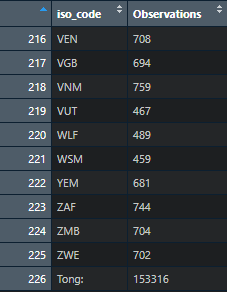
\includegraphics[]{Images/I/I5.png}
		\end{center}
	\end{figure}
		\newpage
		%%%%%%i6)%%%%%%%%%%
		\item Cho biết các châu lục nào có lượng dữ liệu thu thập nhỏ nhất và giá trị nhó nhất đó?
		\begin{figure}[h!]
		\begin{center}
		    
\includegraphics[scale=0.98]{Images/I/I6.png}
		\end{center}
	    \end{figure}
		
		%%%%%%i7)%%%%%%%%%%
		\item Cho biết các châu lục nào có lượng dữ liệu thu thập lớn nhất và giá trị lớn nhất đó?
		\begin{figure}[h!]
		\begin{center}
		    
\includegraphics[]{Images/I/I7.png}
		\end{center}
	    \end{figure}
		
		%%%%%%i8)%%%%%%%%%%
		\item Cho biết các nước nào có lượng dữ liệu thu thập nhỏ nhất và giá trị nhó nhất đó?
		
		%%%%%%i9)%%%%%%%%%%
		\item Cho biết các nước nào có lượng dữ liệu thu thập lớn nhất và giá trị lớn nhất đó?
		\begin{lstlisting}[frame=single]  
coun_data <- as.numeric(table(data$location))
coun <- sort(unique(data$location))
coun_data <- data.frame(cbind(coun,coun_data))
colnames(coun_data) <- c("Country", "Observations")
rownames(coun_data) <- c(1:nrow(coun_data))
coun_data[,2] <- as.numeric(coun_data[,2])
View(rbind(subset(coun_data, 
                  Observations == min(coun_data$Observations)),
           subset(coun_data, 
                  Observations == max(coun_data$Observations))))
	\end{lstlisting}
\begin{itemize}
    \item Ta cũng dùng hàm $table$ tương tự như câu i-5 tuy nhiên thay vì cột $iso\_code$ thì lần này ta sẽ dùng cột $Location$ để lấy tên của đất nước. Sau đó dùng $subset$ để lọc ra các hàng đạt giá trị nhỏ nhất và lớn nhất của data chứa số lượng dữ liệu thu thập được của mỗi nước và xuất ra màn hình.
\end{itemize}
	
	\begin{figure}[h!]
		\begin{center}
		    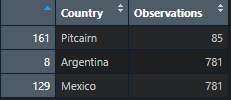
\includegraphics[]{Images/I/I8+9.png}
		\end{center}
	\end{figure}
		
		%%%%%%i10+i11)%%%%%%%%%%
		\item Cho biết các date nào có lượng dữ liệu thu thập nhỏ nhất và giá trị nhó nhất đó?
		\item Cho biết các date nào có lượng dữ liệu thu thập lớn nhất và giá trị lớn nhất đó?
		
		\begin{lstlisting}[frame=single]  
i10_i11 <- function()
{
  date <- c(data$date)
  iso_code <- c(data$iso_code)
  Date <- data.frame(iso_code,date)
  
  Date <- Date %>% arrange(mdy(Date$date))
  df <- data.frame(setDT(Date)[,list(numData=.N),Date$date])
  #i10
  output_i10 = subset(df, numData == min(numData))
  View(output_i10)
  #i11
  output_i11 = subset(df, numData == max(numData))
  View(output_i11)
}
	\end{lstlisting}
	
	
	\begin{itemize}
    \item Hàm $arrange$ từ thư viện $lubridate$ có tác dụng sắp xếp ngày trong data frame Date theo thứ tự từ ngày cũ nhất đến ngày mới nhất
    \item Dòng code tiếp theo có tác dụng sử dụng data frame Date truyền vào, tạo một danh sách $numData$ là số lượng dữ liệu theo từng ngày của data frame Date sau đó tạo một data frame df mới chứa ngày $Date$ và số lượng dữ liệu thu nhập được $numData$
    \item Cuối cùng ta lần lượt tạo các biến $output\_i10$,$output\_i11$ gán lần lượt các subset (tập con) là những ngày có số lượng thu thập dữ liệu thấp nhất và những ngày có lượng thu thập dữ liệu cao nhất
  \end{itemize}
	\begin{figure}[h!]
		\begin{center}
		    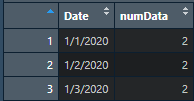
\includegraphics[]{Images/I/I10.png}
		\end{center}
	\end{figure}
		
		\begin{figure}[h!]
		\begin{center}
		    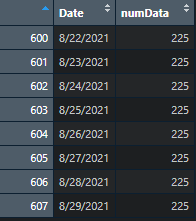
\includegraphics[]{Images/I/I11.png}
		\end{center}
	\end{figure}
	\newpage
		%%%%%%i12+i13+i14)%%%%%%%%%%
		\item Cho biết số lượng dữ liệu thu thập được theo date và châu lục.
		\item Cho biết số lượng dữ liệu thu thập được là lớn nhất theo date và châu lục.
		\item Cho biết số lượng dữ liệu thu thập được là nhỏ nhất theo date và châu lục.
		
		\begin{lstlisting}[frame=single]  
i12_i13_i14 <- function()
{
  df <- data.frame(data)
  df <- subset(df, continent != "")
  date_sort <- df %>% arrange(mdy(df$date))
  #View(date_sort)
  output_i12 <- date_sort %>% group_by(date, continent) 
                          %>% summarise(value = n())
  output_i12 <- output_i12 %>% arrange(mdy(output_i12$date))
  #i12
  View(output_i12)
  #i13
  output_i13 <- subset(output_i12, value == max(value))
  View(output_i13)
  #i14
  output_i14 <- subset(output_i12, value == min(value))
  View(output_i14)
}
	\end{lstlisting}
	
	\begin{figure}[h!]
		\begin{center}
		    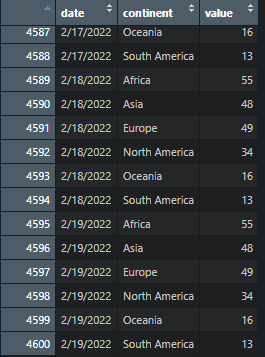
\includegraphics[width=6cm,height=9cm]{Images/I/I12.png}
		    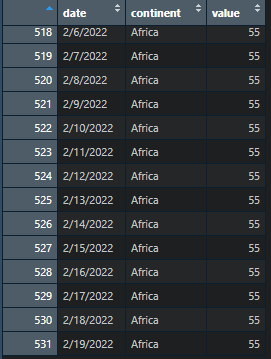
\includegraphics[width=6cm,height=9cm]{Images/I/I13.png}
		\end{center}
		\begin{center}
		    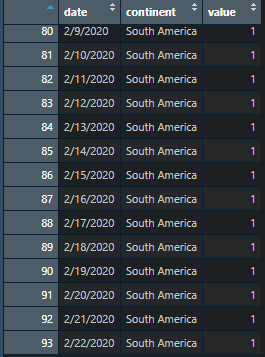
\includegraphics[width=6cm,height=9cm]{Images/I/I14.png}
		\end{center}
	\end{figure}
	\begin{itemize}
	    \item Biến df chứa dữ liệu của tất cả continent có giá trị khác "".\\
	    \item Biến date\_sort chứa dữ liệu ngày tháng năm được sắp xếp bằng hàm $arrange$ theo date.\\
	    \item Biến output\_i12 chứa dữ liệu đầu ra cho mục i câu 12. Bằng cách nhóm date và continent lại và sau đó sử dụng hàm $summarise(value = n())$ để xét trong ngày đó có châu lục nào xuất hiện và nó xuất hiện bao nhiêu lần trong ngày.\\
	    \item Sử dụng lại dữ liệu từ output\_i12 để tìm giá trị lớn nhất và nhỏ nhất theo yêu cầu đề bài.\\
	\end{itemize}

		%%%%%%i15)%%%%%%%%%%
		\newpage
		\item Với một date là k và châu lục t cho trước, hãy cho biết số lượng dữ liệu thể hiện thu thập dữ liệu được.
		\begin{lstlisting}[frame=single]  
df <- data.frame(iso_code, continent,date, new_cases,death_cases)
df$date<-as.Date(df$date,format="%m/%d/%Y") 
k=readline(prompt="Enter the k date with format %Y/%m/%d: ")
t=readline(prompt="Enter the t continent: ")
datefilter = as.Date(k)
df <- df %>% filter(continent == t &date == datefilter)
print(df)
	\end{lstlisting}
	
	\newpage
	 \begin{itemize}
	 \item Ta tạo một data frame df mới, hàm $as.Date$ có tác dụng chuyển vector date trong df từ kiểu dữ liệu $char$ sang $Date$.
	  \item hàm $readline$ để đọc dữ liệu từ bàn phím sau đó gắn giá trị dữ liệu vừa nhập vào các biến k,t
	  \item sử dụng biến datefilter gán giá trị k vừa đươc chuyển đổi sang kiểu dữ liệu $Date$. Sau đó dùng hàm $filter$ để lọc dữ liệu các châu lục và ngày theo k và t cho trước
	 \end{itemize}
		\begin{figure}[h!]
		\begin{center}
		    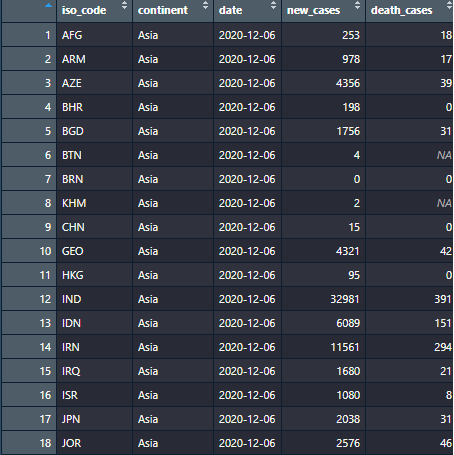
\includegraphics[scale=1.2]{Images/I/i15.png}
		\end{center}
	\end{figure}
		%%%%%%i16)%%%%%%%%%%
		\item Có đất nước nào mà số lượng dữ liệu thu thập được là bằng nhau không? Hãy cho biết các iso\_code của đất nước đó.
		\begin{lstlisting}[frame=single]  
sub_con_data <- subset(con_data,duplicated(con_data[,2])|
                       duplicated(con_data[,2],fromLast=TRUE))
sub_con_data <- sub_con_data[order(sub_con_data[,2]),]
View(sub_con_data)
	\end{lstlisting}
\begin{itemize}
    \item Ta tái sử dụng lại dữ liệu từ biến $con\_data$ của câu i-5. Thông qua điều kiện $duplicated(con_data[,2]) | duplicated(con_data[,2],fromLast=TRUE)$ sẽ giúp ta lấy được tất cả các hàng có dữ liệu trùng lặp với nhau. Ta đưa dữ liệu mới này vào biến $sub\_con\_data$ sau đó sắp xếp lại theo thứ tự tăng dần để dễ nhận biết các nước có số lượng dữ liệu giống nhau.
    \item Vì có rất nhiều nước có lượng dữ liệu thu thập giống nhau nên bên dưới đây chỉ là ảnh minh họa cho một vài nước.
\end{itemize}
	\begin{figure}[h!]
		\begin{center}
		    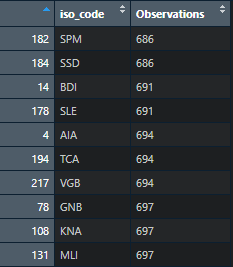
\includegraphics[scale=1.5]{Images/I/I16.png}
		\end{center}
	\end{figure}
		
		
		%%%%%%i17)%%%%%%%%%%
		\newpage
		\item Liệt kê iso\_code, tên đất nước mà chiều dài iso\_code lớn hơn 3.
		\begin{lstlisting}[frame=single]  
i17 <- function()
{
temp <- cbind(unique(data$iso_code),unique(data$location))
output_i17 <- temp[nchar(unique(data$iso_code))>3,]
View(output_i17)
}
	\end{lstlisting}
	\begin{itemize}
	    \item Ta sử dụng hàm $unique$ để lấy các giá trị iso\_code và location chỉ xuất hiện 1 lần trong data và dùng $cbind$ gán vào biến temp. Cuối cùng gán các hàng có iso\_code lớn hơn 3 dùng $nchar$ để đặt điều kiện. 
	\end{itemize}
	\begin{figure}[h!]
		\begin{center}
		    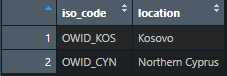
\includegraphics[]{Images/I/I17.png}
		\end{center}
	\end{figure}
\end{enumerate}

%%%%%%ii%%%%%%%%%%%%
\item \textcolor{orange}{Nhóm câu hỏi liên quan đến mô tả thống kê cơ bản dữ liệu}\\
Với mỗi quốc gia mà thuộc về nhóm cần tính số liệu thống kê lần lượt cho nhiễm và tử vong do coronavirus được báo cáo mới:
\begin{enumerate}[1)]

    %%%%%%%%%ii1)%%%%%%%%%%%%%
    \item Tính giá trị nhỏ nhất, lớn nhất
    
    %%%%%%%%%%%%%ii2)%%%%%%%%%
    \item Tính tứ phân vị thứ nhất(Q1), thứ hai(Q2), thứ ba(Q3) 
    
    %%%%%%%%%%%%%ii3)%%%%%%%%%
    \item Tính giá trị trung bình (Avg)
    
    %%%%%%%%%%%%%ii4)%%%%%%%%%
    \item Tính giá trị độ lệch chuẩn (Std)
    
    %%%%%%%%%%%%%ii5)%%%%%%%%%
    \item Đếm xem có bao nhiêu outliers, một quan sát mà giá trị của nó nằm trong khoảng sau:\\
    $IQR = Q3 - Q1$\\
    $outliers < Q1 - 1.5*IQR$ hoặc $outliers > Q3 + 1.5*IQR$
    
    %%%%%%%%%%%%%ii6)%%%%%%%%%
    \item Lập bảng mô tả số liệu thống kê cho từng đất nước thuộc về nhóm: \\
\begin{center}
      \begin{tabular}{ c c c c c c c c c}
        Countries & Min & Q1 & Q2 & Q3 & Max & Avg & Std & Outlier \\ 
        ctr\_i & ? & ? & ? & ? & ? & ? & ? & ? \\ 
      \end{tabular}
    \end{center}
    \begin{lstlisting}[frame=single]
ii <- function(subdata, col)
{
  sum <- summary(subdata[,col])
  min <- as.numeric(sum[1])
  max <- as.numeric(sum[6])
  Q1 <- as.numeric(sum[2])
  Q2 <- as.numeric(sum[3])
  Q3 <- as.numeric(sum[5])
  avg <- as.numeric(sum[4])
  std <- sd(subdata[,col],na.rm = TRUE)
  outlier <- 0
  for(i in 1:nrow(subdata))
  {
    if(is.na(subdata[i,col])) next
    if(subdata[i,col] < (Q1 - (1.5*(Q3 - Q1))) || 
                         subdata[i,col] > (Q3 + (1.5*(Q3 - Q1))))
    {
      outlier <- outlier + 1
    }
    else {}
  }
  return(as.numeric(c(min,Q1,Q2,Q3,max,avg,std,outlier)))
}
dfCountry <- data.frame(Countries = c("Indonesia", 
                                      "Japan", "Vietnam"))
id_data <- subset(data, location == "Indonesia")
jp_data <- subset(data, location == "Japan")
vn_data <- subset(data, location == "Vietnam")

tmp <- data.frame(rbind(ii(id_data,5),ii(jp_data,5),ii(vn_data,5)))
colnames(tmp) <- c("Min", "Q1", "Q2", "Q3",
                   "Max", "Avg", "Std", "Outlier")
dfCountry_case <- cbind(dfCountry,tmp)
View(dfCountry_case)

tmp <- data.frame(rbind(ii(id_data,6),ii(jp_data,6),ii(vn_data,6)))
colnames(tmp) <- c("Min", "Q1", "Q2", "Q3", 
                "Max", "Avg", "Std", "Outlier")
dfCountry_death <- cbind(dfCountry,tmp)
View(dfCountry_death)
	\end{lstlisting}
\begin{itemize}
    \item Ta thực hiện viết hàm $ii()$ để nhận vào data frame của quốc gia và cột tương ứng cần tính. Hàm này sẽ trả về 1 vector có các giá trị tương ứng theo thứ tự là $Min$, $Q1$, $Q2$, $Q3$, $Max$, $Average$, $StandardDeviation$, $Outlier$. Với đó, ta sẽ làm đc cùng lúc toàn bộ các câu từ 1 đến 6 của phần ii.
    \item Bên trong hàm $ii$, ta thực hiện hàm $summary()$ cho cột thứ $col$ nhập vào của dữ liệu đưa vào biến $subdata$. Hàm này sẽ cho ta biết được các giá trị nhỏ nhất, lớn nhất, tứ phân vị và giá trị trung bình của dữ liệu nhập vào. Ta chỉ việc trích xuất các giá trị này vào các biến $min$, $max$, $Q1$, $Q2$, $Q3$, $avg$ tương ứng.
    \item Đối với độ lệch chuẩn $std$ ta thực hiện hàm $sd()$ với $na.rm = TRUE$ để tính độ lệch chuẩn của dữ liệu trong khi bỏ qua các số liệu NA.
    \item Đối với $outlier$, ta khởi tạo giá trị 0. Sau đó thực hiện một vòng lặp for chạy xuyên suốt các hàng của dữ liệu nhập vào. Nếu dữ liệu không phải là NA và thỏa mãn điều kiện $outliers < Q1 - 1.5*IQR$ hoặc $outliers > Q3 + 1.5*IQR$ với $IQR = Q3 - Q1$ thì ta tăng giá trị của $outlier$ lên 1.
    \item Ghép các giá trị này vào 1 vector để hàm trả về.
    \item Bên ngoài hàm, ta thực hiện việc tạo 1 vector $dfCountry$ chứ giá trị là tên của 3 nước thuộc về nhóm cần tính số liệu, sau đó tạo ra các data frame riêng để chứa dữ liệu của từng nước thông qua hàm $subset()$.
    \item Ta sử dụng hàm vừa làm ban nãy để tính tất cả các số liệu cần thiết cho cột $new\_case$ của cả 3 quốc gia thuộc về nhóm cần tính số liệu và ghép lại thành 1 data frame với tên biến $tmp$. Sau đó đặt tên từng cột theo các số liệu tương ứng.
    \item Ta ghép cột $dfCountry$ với data frame vừa tạo để hoàn chỉnh báng số liệu và xuất ra màn hình.
    \item Đối với cột $new\_death$ cũng thực hiện giống như trên chỉ cần thay giá trị thành số thứ tự của cột $new\_death$ vào hàm $ii$
\end{itemize}

	\begin{figure}[h!]
		\begin{center}
		    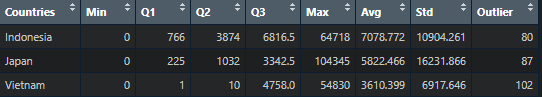
\includegraphics[scale=0.75]{Images/II/ii1-6.png}
		    \label{fig:my_label}
		\end{center}
	\end{figure}
	\begin{figure}[h!]
        \begin{center}
    	    \caption{Số liệu thống kê cho ca nhiễm của từng đất nước}
    	\end{center}
    \end{figure}
	\begin{figure}[h!]
		\begin{center}
		    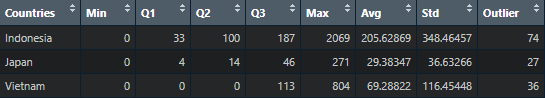
\includegraphics[scale=0.75]{Images/II/ii1-6''.png}
		    \label{fig:my_label}
		\end{center}
	\end{figure}
    \begin{figure}[h!]
        \begin{center}
    	    \caption{Số liệu thống kê cho tử vong của từng đất nước}
    	\end{center}
    \end{figure}
    %%%%%%%%%%%%%ii7)%%%%%%%%%
    \item Vẽ biểu đồ boxplot hay còn được gọi là box-and-whisker cho nhiễm coronavirus
    \begin{lstlisting}[frame=single]  
boxplot(id_data[,5], jp_data[,5], vn_data[,5],
        main = "Plotbox for new cases",
        at = c(1,2,3),
        names = c("Indonesia", "Japan", "Vietnam"),
        col = c("orange","red","yellow"),
        border = "black",
        horizontal = TRUE,
        notch = TRUE
)
boxplot(id_data[,6], jp_data[,6], vn_data[,6],
        main = "Plotbox for new deaths",
        at = c(1,2,3),
        names = c("Indonesia", "Japan", "Vietnam"),
        col = c("orange","red","yellow"),
        border = "black",
        horizontal = TRUE,
        notch = TRUE
)
	\end{lstlisting}
	\begin{figure}[h!]
		\begin{center}
		    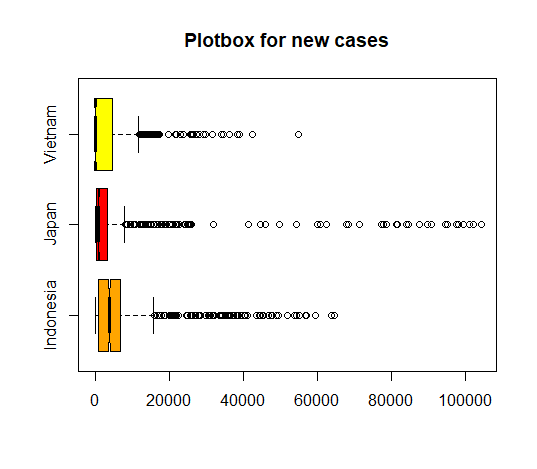
\includegraphics[scale=0.8]{Images/II/ii7.png}
		\end{center}
	\end{figure}
	\begin{figure}[h!]
	    \begin{center}
		    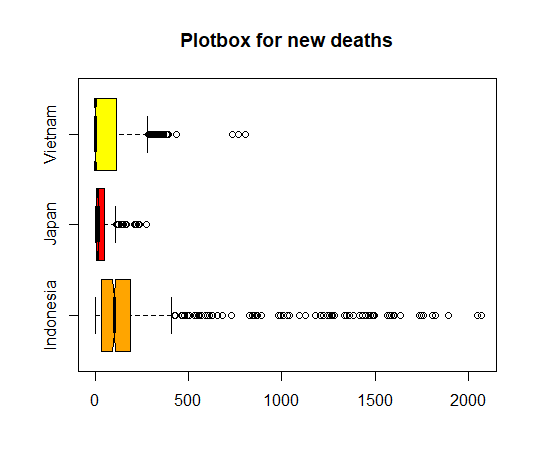
\includegraphics[scale=0.8]{Images/II/ii7death.png}
		\end{center}
	\end{figure}
    
\end{enumerate}
\newpage
\item \textcolor{orange}{Nhóm câu hỏi liên quan đến dữ liệu thể hiện thu thập dữ liệu}\\
Với mỗi quốc gia mà thuộc về nhóm cần tính số liệu thống kê lần lượt cho nhiễm và tử vong do coronavirus:
\begin{enumerate}[1)]
\begin{lstlisting}[frame=single]  
indo <- data[data[,1]=="IDN",]
vn <- data[data[,1]=="VNM",]
jp <- data[data[,1]=="JPN",]
	\end{lstlisting}
	\begin{itemize}
	    \item Tạo data của mỗi quốc gia indonesia, vietnam và japan.
	\end{itemize}
	%%%%%%%%%%iii1)%%%%%%%%
    \item Có bao nhiêu ngày có số lần dữ liệu không được báo cáo mới
    \begin{lstlisting}[frame=single]  
nnreportcindo <- indo[is.na(indo[,5]) | indo[,5]==0,]
indo1.1 <- nrow(nnreportcindo)
view(indo1.1)
nnreportdindo <- indo[is.na(indo[,6]) | indo[,6]==0,]
indo1.2 <- nrow(nnreportdindo)
view(indo1.2)

nnreportcvn <- vn[is.na(vn[,5]) | vn[,5]==0,]
vn1.1 <- nrow(nnreportcvn)
view(vn1.1)
nnreportdvn <- indo[is.na(vn[,6]) | vn[,6]==0,]
vn1.2 <- nrow(nnreportdvn)
view(vn1.1)

nnreportcjp <- jp[is.na(jp[,5]) | jp[,5]==0,]
jp1.1 <- nrow(nnreportcjp)
view(jp1.1)
nnreportdjp <- jp[is.na(jp[,6]) | jp[,6]==0,]
jp1.2 <- nrow(nnreportdjp)
view(jp1.1)
)
	\end{lstlisting}
	\begin{itemize}
	    \item Ta tìm các dữ liệu không được báo cáo mới bằng cách đặt điều kiện bằng 0 và hàm $is.na$ gán vào biến. Sau đó dùng hàm $nrow$ để đếm số hàng của biến.
	\end{itemize}
	\begin{figure}[h!]
		\begin{center}
		    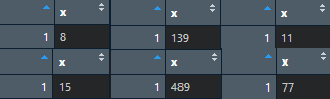
\includegraphics[scale=1.5]{Images/III/iii1.png}
		\end{center}
	\end{figure}.
    
    %%%%%%%%%%iii2)%%%%%%%%
    \item Có bao nhiêu ngày có số ca nhiễm/ tử vong là thấp nhất được báo cáo mới.
    \begin{lstlisting}[frame=single]  
newreportindo <- indo[!is.na(indo[,5]) & !is.na(indo[,6]) 
                      & indo[,5]!=0 & indo[,6]!=0,]
newreportvn <- vn[!is.na(vn[,5]) & !is.na(vn[,6]) 
                  & vn[,5]!=0 & vn[,6]!=0,]
newreportjp <- jp[!is.na(jp[,5]) & !is.na(jp[,6]) 
                  & jp[,5]!=0 & jp[,6]!=0,]
newreport <- rbind(newreportindo,newreportvn,newreportjp)

indominc <- newreportindo[newreportindo[,5]==min(newreportindo[,5]),4]
indo2.1 <- length(indominc)
view(indo2.1)
indomind <- newreportindo[newreportindo[,6]==min(newreportindo[,6]),4] 
indo2.2 <- length(indomind)
view(indo2.2)

vnminc <- newreportvn[newreportvn[,5]==min(newreportvn[,5]),4] 
vn2.1 <- length(vnminc)
view(vn2.1)
vnmind <- newreportvn[newreportvn[,6]==min(newreportvn[,6]),4] 
vn2.2 <- length(vnmind)
view(vn2.2)

jpminc <- newreportjp[newreportjp[,5]==min(newreportjp[,5]),4] 
jp2.1 <- length(jpminc)
view(jp2.1)
jpmind <- newreportjp[newreportjp[,6]==min(newreportjp[,6]),4] 
jp2.2 <- length(jpmind)
view(jp2.2)
	\end{lstlisting}
	\begin{itemize}
	    \item Tương tự tìm các dữ liệu được báo cáo mới gán vào biến. Sau dó dùng hàm $min$ để tìm giá trị thấp nhất và đặt điều kiện trong matrix để tìm các ngày bằng giá trị đó. Cuối cùng dùng hàm $length$ để tìm số ngày có giá trị thấp nhất được báo cáo mới.
	\end{itemize}
	\begin{figure}[h!]
		\begin{center}
		    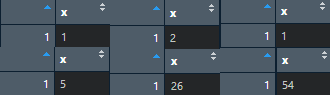
\includegraphics[scale=1.5]{Images/III/iii2.png}
		\end{center}
	\end{figure}.
    
    %%%%%%%%%%iii3)%%%%%%%%
    \item Có bao nhiêu ngày có số ca nhiễm/ tử vong là cao nhất được báo cáo mới
    \begin{lstlisting}[frame=single]  
indomaxc <- newreportindo[newreportindo[,5]==max(newreportindo[,5]),4] 
indo3.1 <- length(indomaxc)
view(indo3.1)
indomaxd <- newreportindo[newreportindo[,6]==max(newreportindo[,6]),4] 
indo3.2 <- length(indomaxd)
view(indo3.2)

vnmaxc <- newreportvn[newreportvn[,5]==max(newreportvn[,5]),4] 
vn3.1 <- length(vnmaxc)
view(vn3.1)
vnmaxd <- newreportvn[newreportvn[,6]==max(newreportvn[,6]),4] 
vn3.2 <- length(vnmaxd)
view(vn3.2)

jpmaxc <- newreportjp[newreportjp[,5]==max(newreportjp[,5]),4] 
jp3.1 <- length(jpmaxc)
view(jp3.1)
jpmaxd <- newreportjp[newreportjp[,6]==max(newreportjp[,6]),4] 
jp3.2 <- length(jpmaxd)
view(jp3.2)
	\end{lstlisting}
	\begin{figure}[h!]
		\begin{center}
		    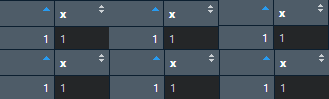
\includegraphics[scale=1.5]{Images/III/iii3.png}
		\end{center}
	\end{figure}.
    \newpage
    %%%%%%%%%%iii4)%%%%%%%%
    \item Thể hiện bảng số liệu như sau:\\
    Không được báo cáo mới:
    \begin{center}
      \begin{tabular}{ c c c }
        Countries & Infections & Deaths \\ 
        ctr\_i & value  & value\\ 
      \end{tabular}
    \end{center}
    Báo cáo mới:
    \begin{center}
      \begin{tabular}{ c c c }
        Countries & Infections & Deaths \\ 
        ctr\_i & value  & value\\ 
      \end{tabular}
    \end{center}
    \begin{lstlisting}[frame=single]  
nnreport <- rbind(indo[is.na(indo[,5]) | is.na(indo[,6]) 
                       | indo[,6]==0 | indo[,5]==0,],
                  vn[is.na(vn[,5]) | is.na(vn[,6]) 
                     | vn[,5]==0 | vn[,6] ==0,],
                  jp[is.na(jp[,5]) | is.na(jp[,6]) 
                     | jp[,5]==0 | jp[,6]==0,]) 
iii4.1 <- nnreport[,-c(1,2,4)]
colnames(iii4.1) <- c("Countries","Infections value","Deaths value")
view(iii4.1)
iii4.2 <- newreport[,-c(1,2,4)]
colnames(iii4.2) <- c("Countries","Infections value","Deaths value")
view(iii4.2)
	\end{lstlisting}
	\begin{itemize}
	    \item Đặt điều kiện trong matrix để tìm các dữ liệu không được báo cáo mới của 3 nước và dùng $rbind$ để gán các dữ liệu đó vào biến nnreport. Sau đó lấy các cột 1, 2, 4 của data nnreport và gán vào biến mới. Cuối cùng dùng hàm $colnames$ để đổi tên cho cột.
	\end{itemize}
	\begin{figure}[h!]
		\begin{center}
		    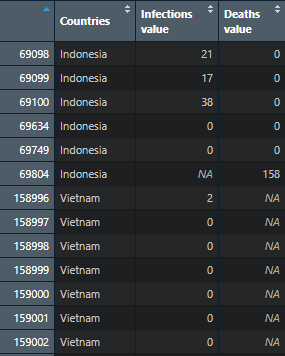
\includegraphics[scale=0.65]{Images/III/iii4.1.png}
		    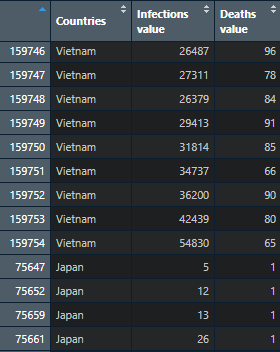
\includegraphics[scale=0.65]{Images/III/iii4.2.png}
		\end{center}
	\end{figure}.
	
    %%%%%%%%%%iii5)%%%%%%%%
    \item Cho biết số ngày ngắn nhất liên tiếp mà không có dữ liệu được báo cáo
    \begin{lstlisting}[frame=single]  
indo5_case <- 0
for (i in 1:nrow(indo)){
  if (is.na(indo[i,5])){
    indo5_case <- indo5_case + 1
    break
  }
}
view(indo5_case)
indo5_death <- 0
for (i in 1:nrow(indo)){
  if (is.na(indo[i,6])){
    indo5_death <- indo5_death + 1
    break
  }
}
view(indo5_death)

vn5_case <- 0
for (i in 1:nrow(vn)){
  if (is.na(vn[i,5])){
    vn5_case <- vn5_case + 1
    break
  }
}
view(vn5_case)
vn5_death <- 0
for (i in 1:nrow(vn)){
  if (is.na(vn[i,6])){
    vn5_death <- vn5_death + 1
    break
  }
}
view(vn5_death)

jp5_case <- 0
for (i in 1:nrow(jp)){
  if (is.na(jp[i,5])){
    jp5_case <- jp5_case + 1
    break
  }
}
view(jp5_case)
jp5_death <- 0
for (i in 1:nrow(jp)){
  if (is.na(jp[i,6])){
    jp5_death <- jp5_death + 1
    break
  }
}
view(jp5_death)
	\end{lstlisting}
	\begin{itemize}
	    \item Ta chạy vòng for và dùng hàm $is.na$ để kiểm tra giá trị của cột 5,6 của data mỗi nước. Nếu $TRUE$ thì kết quả là 1, ngược lại kết quả bằng 0.
	\end{itemize}
	\begin{figure}[h!]
		\begin{center}
		    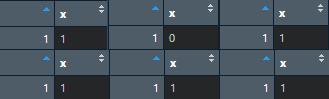
\includegraphics[scale=1.5]{Images/III/iii5.png}
		\end{center}
	\end{figure}.
    
    %%%%%%%%%%iii6)%%%%%%%%
    \item Cho biết số ngày dài nhất liên tiếp mà không có dữ liệu được báo cáo
    
    \begin{lstlisting}[frame=single]  
indo6_case <- 0
temp <- 0
for (i in 1:nrow(indo)){
  if (is.na(indo[i,5])){
    temp <- temp + 1
    if (temp>indo6_case) {
      indo6_case <- temp
    }
  }
  else{
    temp <- 0
  }
}
view(indo6_case)
indo6_death <- 0
temp <- 0
for (i in 1:nrow(indo)){
  if (is.na(indo[i,6])){
    temp <- temp + 1
    if (temp>indo6_death) {
      indo6_death <- temp
    }
  }
  else{
    temp <- 0
  }
}
view(indo6_death)

vn6_case <- 0
temp <- 0
for (i in 1:nrow(vn)){
  if (is.na(vn[i,5])){
    temp <- temp + 1
    if (temp>vn6_case) {
      vn6_case <- temp
    }
  }
  else{
    temp <- 0
  }
}
view(vn6_case)
vn6_death <- 0
temp <- 0
for (i in 1:nrow(vn)){
  if (is.na(vn[i,6])){
    temp <- temp + 1
    if (temp>vn6_death) {
      vn6_death <- temp
    }
  }
  else{
    temp <- 0
  }
}
view(vn6_death)

jp6_case <- 0
temp <- 0
for (i in 1:nrow(jp)){
  if (is.na(jp[i,5])){
    temp <- temp + 1
    if (temp>jp6_case) {
      jp6_case <- temp
    }
  }
  else{
    temp <- 0
  }
}
view(jp6_case)
jp6_death <- 0
temp <- 0
for (i in 1:nrow(jp)){
  if (is.na(jp[i,6])){
    temp <- temp + 1
    if (temp>jp6_death) {
      jp6_death <- temp
    }
  }
  else{
    temp <- 0
  }
}
view(jp6_death)
	\end{lstlisting}
	\begin{itemize}
	    \item Ta chạy vòng for và dùng hàm $is.na$ để kiểm tra dữ liệu cột 5,6 của mỗi nước, nếu $TRUE$ biến temp tăng và so sánh vs số ngày dài nhất liên tiếp, nếu $FALSE$ reset biến temp.
	\end{itemize}
	\begin{figure}[h!]
		\begin{center}
		    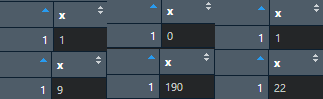
\includegraphics[scale=1.5]{Images/III/iii6.png}
		\end{center}
	\end{figure}.
    
    %%%%%%%%%%iii7)%%%%%%%%
    \item Cho biết số ngày ngắn nhất liên tiếp mà không có người nhiễm bệnh mới
    \begin{lstlisting}[frame=single]  
indo7 <- 0
for (i in 1:nrow(nnreportcindo)){
  if (nnreportcindo[i,5]==0){
    indo7 <- indo7 + 1
    break
  }
}
view(indo7)

vn7 <- 0
for (i in 1:nrow(nnreportcvn)){
  if (nnreportcvn[i,5]==0){
    vn7 <- vn7 + 1
    break
  }
}
view(vn7)

jp7 <- 0
for (i in 1:nrow(nnreportcjp)){
  if (nnreportcindo[i,5]==0){
    jp7 <- jp7 + 1
    break
  }
}
view(jp7)
	\end{lstlisting}
	\begin{figure}[h!]
		\begin{center}
		    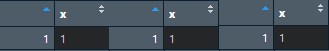
\includegraphics[scale=1.5]{Images/III/iii7.png}
		\end{center}
	\end{figure}.
    
    %%%%%%%%%%iii8)%%%%%%%%
    \item Cho biết số ngày dài nhất liên tiếp mà không có người nhiễm bệnh mới
    \begin{lstlisting}[frame=single]  
indo8 <- 0
temp <- 0
for (i in 1:nrow(indo)){
  if(!is.na(indo[i,5]) & indo[i,5]==0){
    temp <- 0
  }
  else{
    temp <- temp + 1
    if (temp>indo8) {
      indo8 <- temp
    }
  }
}
view(indo8)

vn8 <- 0
temp <- 0
for (i in 1:nrow(vn)){
  if(!is.na(vn[i,5]) & vn[i,5]==0){
    temp <- 0
  }
  else{
    temp <- temp + 1
    if (temp>vn8) {
      vn8 <- temp
    }
  }
}
view(vn8)

jp8 <- 0
temp <- 0
for (i in 1:nrow(jp)){
  if(!is.na(jp[i,5]) & jp[i,5]==0){
    temp <- 0
  }
  else{
    temp <- temp + 1
    if (temp>jp8) {
      jp8 <- temp
    }
  }
}
view(jp8)
	\end{lstlisting}
	\begin{figure}[h!]
		\begin{center}
		    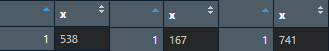
\includegraphics[scale=1.5]{Images/III/iii8.png}
		\end{center}
	\end{figure}.
    
\end{enumerate}

%%%%%%%%%%iv)%%%%%%%%
\item \textcolor{red}{Nhóm câu hỏi liên quan đến trực quan dữ liệu}
\begin{enumerate}[1)]
    \lstset{
    title=Prep for iv1-2}
\begin{lstlisting}[frame=single]  
freg <- data[!duplicated(data[,c('location')]),]
coun_num <- nrow(freg)
x_con <- c("Africa","Asia","Europe",
            "North America","Oceania","South America")
\end{lstlisting}
\begin{itemize}
    \item Ta dùng câu lệnh $data[!duplicated(data[,c('location')]),]$ để loại bỏ các dòng có giá trị lặp ở cột $Location$ để cho ta 1 data mới với mỗi nước chỉ xuất hiện duy nhất 1 lần. Ta bỏ data mới này vào biến $freg$.
    \item Dùng hàm $nrow()$ để đếm tổng số đất nước và bỏ vào biến $coun\_num$.
    \item Tiến hành khởi tạo trước cột x cho biểu đồ với giá trị là tên của từng châu lục.
\end{itemize}


%%%%%%%%%%iv1)%%%%%%%%
    \item Vẽ biểu đồ tần số tích lũy quốc gia cho các châu lục
    \lstset{
    title=Source code}
\begin{lstlisting}[frame=single]  
y_con <- cumsum(as.numeric(table(freg$continent)))
df_iv1 <- data.frame(Continent = x_con,Freg = y_con)
ggplot(data = df_iv1, aes(x = Continent, y = Freg, fill = Continent)) 
        + geom_bar(stat = "Identity", colour = "black")
\end{lstlisting}
\begin{itemize}
    \item Sử dụng hàm $table()$ để đếm số lần xuất hiện của các châu lục. Vì mỗi quốc gia trong data vừa xử lý chỉ xuất hiện duy nhất một lần nên việc ta vừa làm chính là đếm số quốc gia cho từng châu lục
    \item Ta tiếp dụng dùng hàm $cumsum()$ để biến đổi vector này thành dạng tích lũy. Chuyển dữ liệu này thành dạng số và bỏ vào $vector$ cho cột y của biều đồ.
\end{itemize}
\begin{figure}[h!]
	\begin{center}
        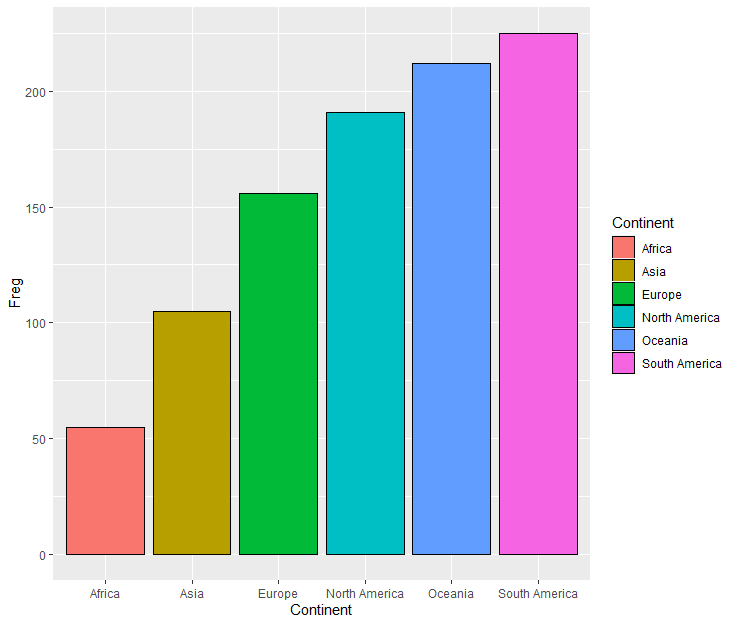
\includegraphics[scale=0.8]{Images/IV/iv (1).png}
	\end{center}
\end{figure}

	%%%%%%%%%%iv2)%%%%%%%%
    \item Vẽ biểu đồ tần số tương đối quốc gia cho các châu lục
    \lstset{
    title=Source code}
\begin{lstlisting}[frame=single]  
y_con <- y_con/coun_num
df_iv2 <- data.frame(Continent = x_con,Freg = y_con)
ggplot(data = df_iv2, aes(x = Continent, y = Freg, fill = Continent)) 
        + geom_bar(stat = "Identity", colour = "black")
\end{lstlisting}
\begin{itemize}
    \item Biến đổi $vector$ cho cột y ở câu trước thành tần số tích lũy bằng cách chia nó cho giá trị cuối cùng của $vector$ hoặc chia cho tổng số quốc gia và tiến hành vẽ biểu đồ như câu trên.
\end{itemize}
\begin{figure}[h!]
	\begin{center}
	    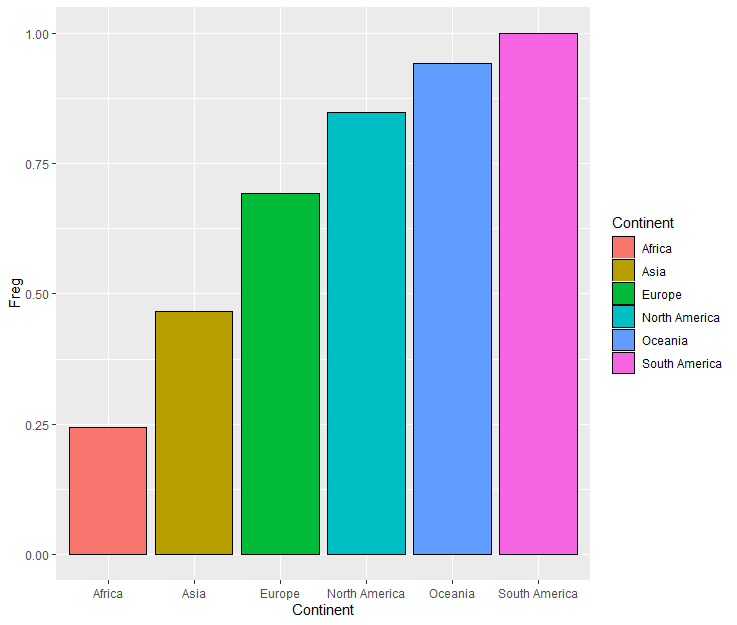
\includegraphics[scale=0.8]{Images/IV/iv (2).png}
	\end{center}
\end{figure}
    \newpage
    \lstset{
    title=Prep for iv3-4}
\begin{lstlisting}[frame=single]  
x_coun <- c("Indonesia","Japan","Vietnam")
id_data <- subset(data, location == "Indonesia")
jp_data <- subset(data, location == "Japan")
vn_data <- subset(data, location == "Vietnam")

id_date <- tail(id_data[order(as.Date(id_data$date,
                format="%d/%m/%Y")),],n=7)
jp_date <- tail(jp_data[order(as.Date(jp_data$date,
                format="%d/%m/%Y")),],n=7)
vn_date <- tail(vn_data[order(as.Date(vn_data$date,
                format="%d/%m/%Y")),],n=7)

dfDate <- data.frame(rbind(id_date,jp_date,vn_date))
\end{lstlisting}
\begin{itemize}
    \item Thực hiện tạo 1 vector $x\_coun$ chứa tên của các quốc gia thuộc về nhóm cần tính số liệu.
    \item Lấy ra dữ liệu của từng quốc gia rồi sử dụng hàm $order(as.Date())$ với format là $dd-mm-yyyy$ để sắp xếp dữ liệu của từng quốc gia theo ngày tăng dần và dùng hàm $tail()$ với $n\ =\ 7$ để lấy ra 7 ngày cuối của năm cuối cùng.
    \item Tiến hành ghép tất cả dữ liệu vừa xử lý của 3 quốc gia lại với nhau. Qua đó ta có thể dễ dàng vẽ biểu đồ nhiễm bệnh hay tử vong của các quốc gia khi chỉ cần thay giá trị của trục y trong câu lệnh $ggplot()$ thành cột dữ liệu tương ứng.
\end{itemize}
\newpage
%%%%%%%%%%iv3)%%%%%%%%
    \item Vẽ biểu đồ thể hiện nhiễm bệnh đã báo cáo của các quốc gia  mà thuộc về nhóm trong 7 ngày cuối của năm cuối cùng
    \lstset{
    title=Source code}
\begin{lstlisting}[frame=single]  
ggplot(data = dfDate, aes(x = location, y = new_cases, fill = date)) 
    + geom_bar(stat = "Identity",colour = "black",position = "dodge")
\end{lstlisting}
\begin{figure}[h!]
	\begin{center}
        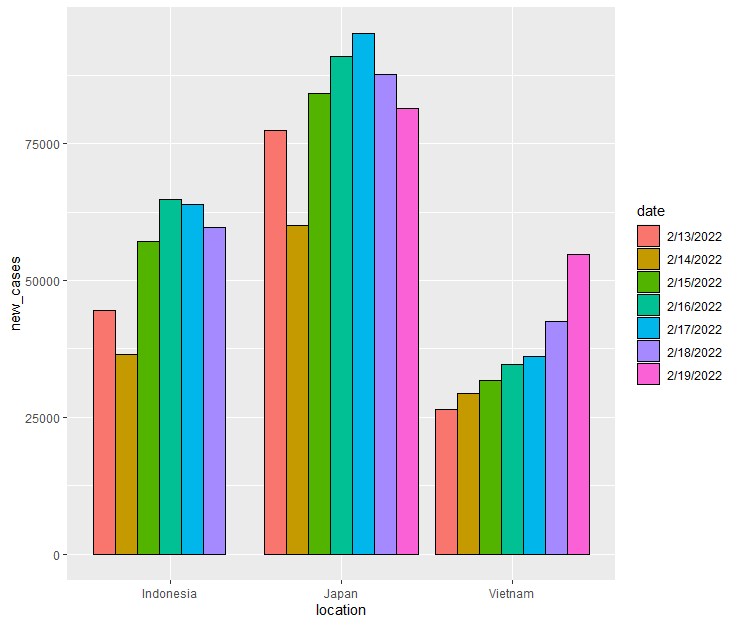
\includegraphics[scale=0.8]{Images/IV/iv (3).png}
	\end{center}
\end{figure}


%%%%%%%%%%iv4)%%%%%%%%
    \item Vẽ biểu đồ thể hiện tử vong đã báo cáo của các quốc gia  mà thuộc về nhóm trong 7 ngày cuối của năm cuối cùng
    \lstset{
    title=Source code}
\begin{lstlisting}[frame=single]  
ggplot(data = dfDate, aes(x = location, y = new_deaths, fill = date)) 
    + geom_bar(stat = "Identity",colour = "black",position = "dodge")
\end{lstlisting}
\begin{figure}[h!]
	\begin{center}
        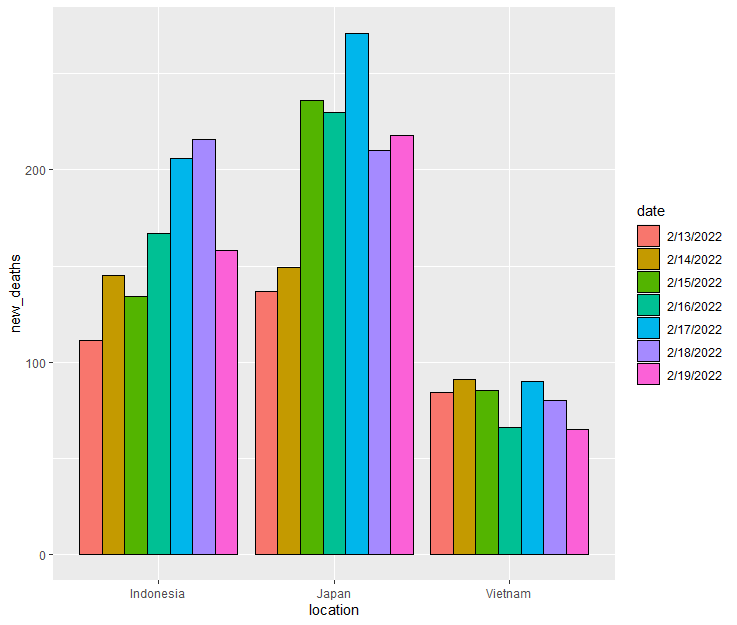
\includegraphics[scale=0.8]{Images/IV/iv (4).png}
	\end{center}
\end{figure}
\newpage
\lstset{
    title=Function and Prep for iv5-6}
\begin{lstlisting}[frame=single]  
iv_5_6 <- function(data, name, col)
{
  subdata <- subset(data,location==name)
  sum <- summary(subdata[,col])
  Q1 <- as.numeric(sum[2])
  Q3 <- as.numeric(sum[5])
  outlier <- 0
  for(i in 1:nrow(subdata))
  {
    if(is.na(subdata[i,col])) next
    if(subdata[i,col] < (Q1 - (1.5*(Q3 - Q1))) 
       || subdata[i,col] > (Q3 + (1.5*(Q3 - Q1))))
    {
      outlier <- outlier + 1
    }
  }
  return(c(name,outlier))
}

coun_name <- unique(data[,3])
\end{lstlisting}
\begin{itemize}
    \item Hàm $iv\_5\_6()$ có tác dụng nhận vào toàn bộ dữ liệu data, tên của quốc gia và cột cần tính outlier. Hàm sẽ trả về 1 $vector$ với 2 giá trị là tên của quốc gia và số outlier của quốc gia đó.
    \item Bên trong hàm sẽ lấy ra những dòng dữ liệu từ $data$ của đất nước cần tính trong biến $name$ và bỏ tất cả vào một $subdata$ mới. Ta lại tiếp tục dùng hàm $summary()$ để lấy tứ phân vị thứ nhất $Q1$ và thứ ba $Q3$. Ta thực hiện chạy 1 vòng lặp for qua tất cả các dòng trong $subdata$ để bắt đầu việc tính outlier.
    \item Ta khởi tạo giá trị của biến $outlier$ bằng 0. Với mỗi hàng ta đi qua, nếu dữ liệu không phải là NA và thỏa mãn điều kiện $outliers < Q1 - 1.5*IQR$ hoặc $outliers > Q3 + 1.5*IQR$ với $IQR = Q3 - Q1$ thì ta tăng giá trị của $outlier$ lên 1.
    \item Bên ngoài hàm, ta thực hiện việc lấy danh sách tên các quốc gia bằng hàm $unique()$.
\end{itemize}
%%%%%%%%%%iv5)%%%%%%%%
    \item Vẽ biểu đồ phổ đất nước xuất hiện outliers cho nhiễm bệnh
    \lstset{
    title=Source code}
\begin{lstlisting}[frame=single]  
dfOutlier <- data.frame(Countries = c("tmp"), Outlier = c(0))
for(i in 1:length(coun_name))
{
  dfOutlier <- rbind(dfOutlier, iv_5_6(data,coun_name[i],5))
}
dfOutlier[,2] <- as.numeric(dfOutlier[,2])
dfOutlier <- subset(dfOutlier, Outlier != 0)
view_dfOutlier <- data.frame(rbind(subset(dfOutlier, 
                                          Countries == "Indonesia"),
                                   subset(dfOutlier, 
                                          Countries == "Japan"),
                                   subset(dfOutlier, 
                                          Countries == "Vietnam")))
ggplot(data = dfOutlier, aes(x = Countries, y = Outlier))
    + geom_bar(stat = "Identity", colour = "black")
ggplot(data = view_dfOutlier, 
       aes(x = Countries, y = Outlier, fill = Countries))
    + geom_bar(stat = "Identity", colour = "black")
\end{lstlisting}
\begin{itemize}
    \item Ta tiến hành tạo 1 data frame mới tên là $dfOutlier$ với 2 cột là $Countries$ và $Outlier$. Khởi tạo giá trị cho dòng đầu tiên của data frame này là $tmp$ và $0$ tương ứng với 2 cột.
    \item Thực hiện 1 vòng lặp for chạy qua toàn bộ từng phần tử của vector $coun\_name$. Với mỗi lần lặp, ta sẽ thực hiện hàm $iv\_5\_6()$ để tính outlier cho ca nhiễm của mỗi đất nước trong vector $coun\_name$ và gắn vector trả về của hàm vào data frame $dfOutlier$. Như vậy sau khi chạy hết vòng for thì $dfOutlier$ đã chứa toàn bộ tên đất nước cũng như số outlier của từng đất nước tương ứng.
    \item Ta tiếp tục biến đổi cột $Outlier$ của $dfOutlier$ thành số để có thể vẽ được biểu đồ đồng thời loại các dòng mà tại quốc gia đó có số outlier là 0. Việc này sẽ giúp ta loại được cả dòng đầu tạm thời của data frame ta đặt khi nãy.
    \item Tiến hành vẽ biểu độ cột dựa trên dữ liệu có được bằng hàm $ggplot()$.
\end{itemize}
\newpage
\begin{figure}[h!]
	\begin{center}
        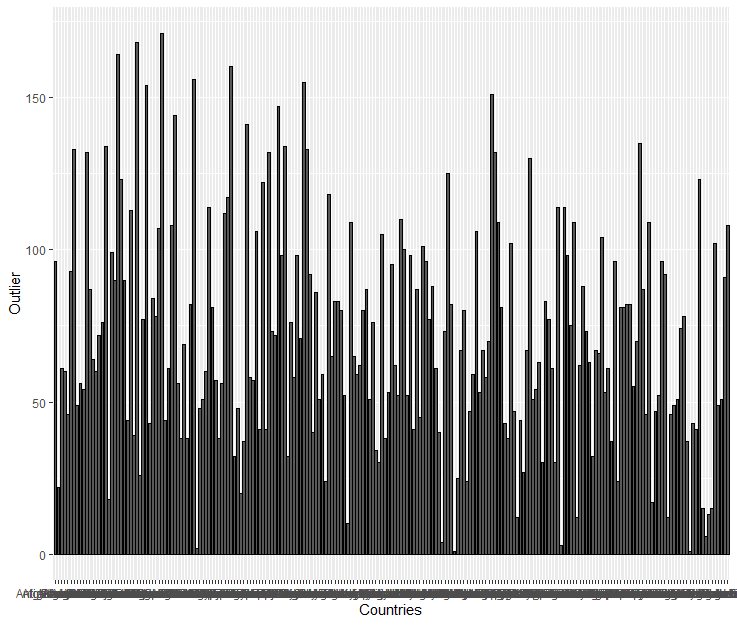
\includegraphics[scale=0.8]{Images/IV/iv (5) - 1.png}
	\end{center}
\end{figure}
\begin{itemize}
    \item Ta dễ dàng nhận thấy vì có quá nhiều đất nước nên việc hiển thị toàn bộ dữ liệu trên biểu đồ sẽ rất khó nhìn. Vậy nên ta sẽ rút gọn lại chỉ với 3 nước thuộc về nhóm cần tính số liệu bằng việc đưa dữ liệu outlier của 3 nước này vào một biến $view\_dfOutlier$ và vẽ biểu đồ cho data frame này.
\end{itemize}
\begin{figure}[h!]
	\begin{center}
        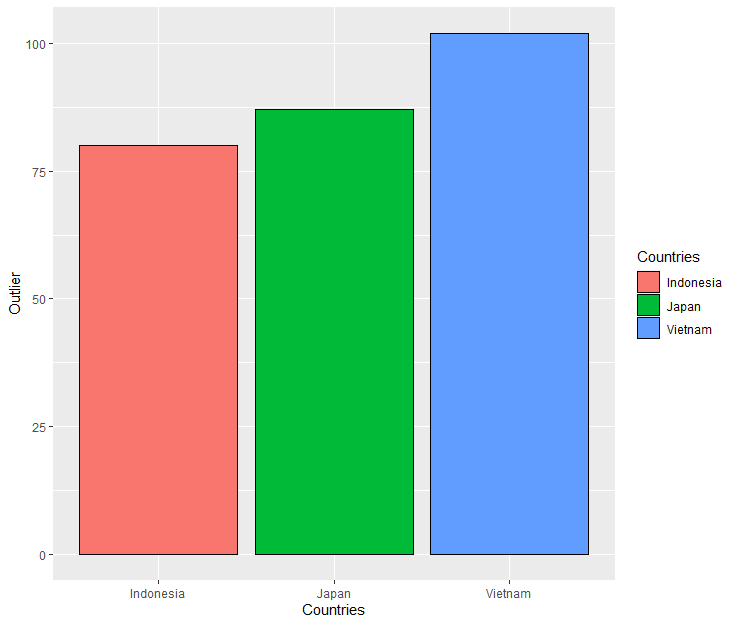
\includegraphics[scale=0.8]{Images/IV/iv (5) - 2.png}
	\end{center}
\end{figure}
\newpage

%%%%%%%%%%iv6)%%%%%%%%
    \item Vẽ biểu đồ phổ đất nước xuất hiện outliers cho tử vong
    \lstset{
    title=Source code}
\begin{lstlisting}[frame=single]  
dfOutlier <- data.frame(Countries = c("tmp"), Outlier = c(0))
for(i in 1:length(coun_name))
{
  dfOutlier <- rbind(dfOutlier, iv_5_6(data,coun_name[i],6))
}
dfOutlier[,2] <- as.numeric(dfOutlier[,2])
dfOutlier <- subset(dfOutlier, Outlier != 0)
view_dfOutlier <- data.frame(rbind(subset(dfOutlier, 
                                    Countries == "Indonesia"),
                                   subset(dfOutlier, 
                                    Countries == "Japan"),
                                   subset(dfOutlier, 
                                    Countries == "Vietnam")))
ggplot(data = dfOutlier, aes(x = Countries, y = Outlier))
    + geom_bar(stat = "Identity", colour = "black")
ggplot(data = view_dfOutlier, aes(x = Countries, y = Outlier, 
        fill = Countries))
    + geom_bar(stat = "Identity", colour = "black")
\end{lstlisting}
\begin{itemize}
    \item Ta cũng tiến hành tạo data frame và vẽ biểu đồ tương tự như câu $iv-5$ nhưng là với outlier cho tử vong của mỗi đất nước bằng hàm $ggplot()$.
\end{itemize}
\begin{figure}[h!]
	\begin{center}
        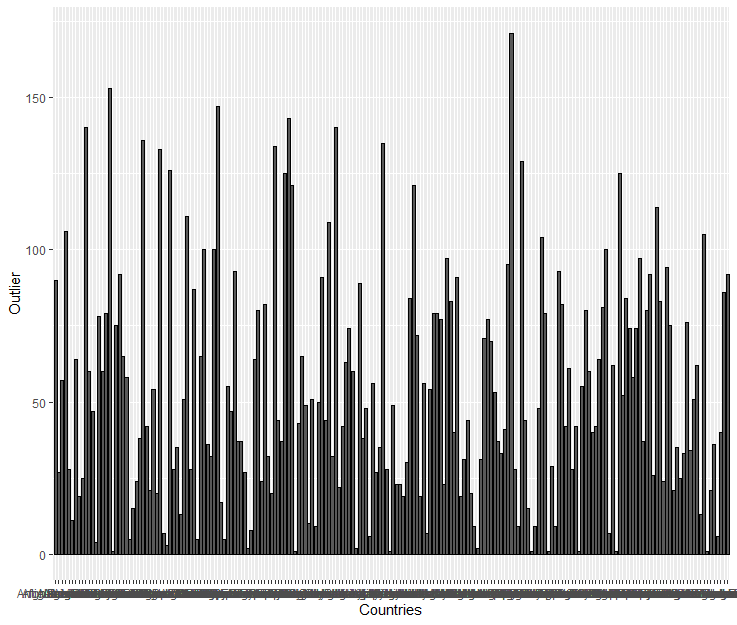
\includegraphics[scale=0.6]{Images/IV/iv (6) - 1.png}
	\end{center}
\end{figure}
\begin{itemize}
    \item Ta cũng dễ dàng nhận thấy vì có quá nhiều đất nước nên việc hiển thị toàn bộ dữ liệu trên biểu đồ sẽ rất khó nhìn. Vậy nên ta sẽ rút gọn lại chỉ với 3 nước thuộc về nhóm cần tính số liệu và vẽ biểu đồ.
\end{itemize}
\begin{figure}[h!]
	\begin{center}
        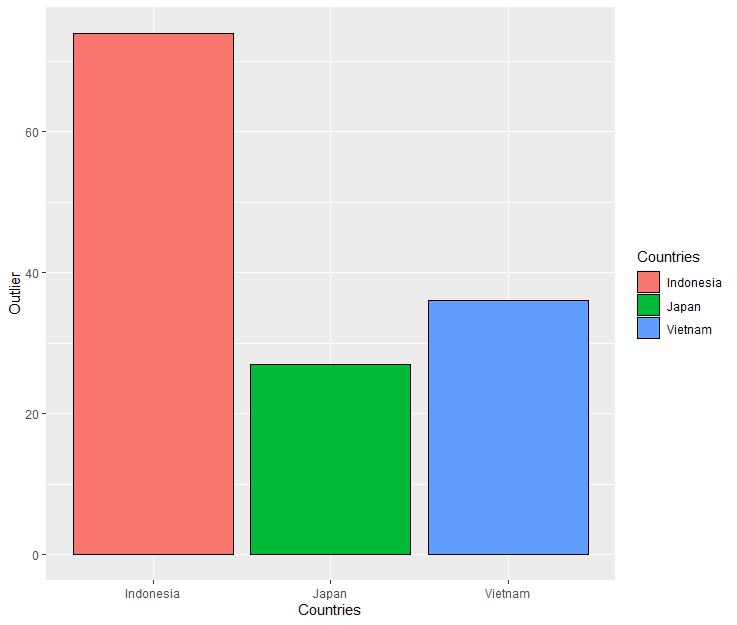
\includegraphics[scale=0.7]{Images/IV/iv (6) - 2.png}
	\end{center}
\end{figure}.

\end{enumerate}
%%%%%%%%%%function v,vi,vii,viii%%%%%%%%
\lstset{
    title=Function and data for v vi vii viii}
\begin{lstlisting}[frame = single]
#MADE
data2 <- data[data[,3]%in%c("Vietnam","Japan","Indonesia"),]
data2 <- rbind(data2,world_data)
data2[,4] <- as.POSIXct(data2[,4], format = "%m/%d/%Y")
y2020 <- data2[format(data2[,4],format="%Y")=="2020" & 
                 (format(data2[,4],format="%m")=="02" | 
                    format(data2[,4],format="%m")=="01" | 
                    format(data2[,4],format="%m")=="07" | 
                    format(data2[,4],format="%m")=="09"),]

y2021 <- data2[format(data2[,4],format="%Y")=="2021" & 
                 (format(data2[,4],format="%m")=="02" | 
                    format(data2[,4],format="%m")=="01" | 
                    format(data2[,4],format="%m")=="07" | 
                    format(data2[,4],format="%m")=="09"),]

y2022 <- data2[format(data2[,4],format="%Y")=="2022" & 
                 (format(data2[,4],format="%m")=="02" | 
                    format(data2[,4],format="%m")=="01" | 
                    format(data2[,4],format="%m")=="07" | 
                    format(data2[,4],format="%m")=="09"),]


#last_month
y2020_1 <- data2[format(data2[,4],format="%Y")=="2020" & 
                   (format(data2[,4],format="%m")=="11" | 
                      format(data2[,4],format="%m")=="12"),]

y2021_1 <- data2[format(data2[,4],format="%Y")=="2021" & 
                   (format(data2[,4],format="%m")=="11" | 
                      format(data2[,4],format="%m")=="12"),]

y2022_1 <- data2[format(data2[,4],format="%Y")=="2022" & 
                   (format(data2[,4],format="%m")=="11" | 
                      format(data2[,4],format="%m")=="12"),]

#function
draw_chart <- function(year_data, month_data, yyyy,
                        cases_or_deaths,avg_or_not="")
{
  if(dim(year_data) == 0)
  return(ggplot()+labs(x="",y=paste(cases_or_deaths,"",yyyy))+
  theme(legend.position="top")+ggtitle("NA"))
 
  amedumb <- 5
  pain <- "Cases"
  if(cases_or_deaths == "deaths"){
    pain <- "Deaths"
    amedumb <- 6 
  }
  if(avg_or_not == "avg")
  {
    tmp <- ave_handle(year_data, month_data, amedumb)
    year_data[,amedumb] <- tmp
  }
  
  chart_out <- ggplot(data=year_data, 
  aes(x=format(year_data[,4],format="%d"),y=year_data[,amedumb],
  color=month_data,group=month_data))+
    geom_line(lwd=1)+
    labs(x="",y=paste(pain,"",yyyy))+
    theme(legend.position="top")
  return(chart_out)
}

cum_rel <- function(year_data, month_data, yyyy, 
                    cases_or_deaths,avg_or_not="")
{
  if(dim(year_data) == 0)
  return(ggplot()+labs(x="",y=paste(cases_or_deaths,"",yyyy))+
  theme(legend.position="top")+ggtitle("NA"))
  amedumb <- 5
  pain <- "Cases"
  if(cases_or_deaths == "deaths"){
    pain <- "Deaths"
    amedumb <- 6 
  }
  if(avg_or_not == "avg")
  {
    tmp <- ave_handle(year_data,month_data,amedumb)
    year_data[,amedumb] <- tmp
  }
  
  cum_sum_data <- cbind(cumsum(year_data[,amedumb]))
  prob <- cum_sum_data/sum(year_data[,amedumb])
  year_data[,amedumb] <- prob
  chart_out <- ggplot(data=year_data, aes(x=year_data[,4],
  y=year_data[,amedumb],group=1))+
    geom_line(lwd=1)+
    labs(x="Dates",y=paste(pain,"_crf",yyyy))+
    scale_x_datetime(date_labels = "%m/%d/%Y",date_breaks = "1 week")+
    theme(legend.position="top")
  return(chart_out)
}

cum <- function(year_data, month_data,yyyy,cases_or_deaths,avg_or_not="")
{
  if(dim(year_data) == 0) return(ggplot()+labs(x="",y=paste(cases_or_deaths,"",yyyy))+
  theme(legend.position="top")+ggtitle("NA"))
  amedumb <- 5
  pain <- "Cases"
  if(cases_or_deaths == "deaths"){
    pain <- "Deaths"
    amedumb <- 6 
  }
  if(avg_or_not == "avg")
  {
    tmp <- ave_handle(year_data, month_data, amedumb)
    year_data[,amedumb] <- tmp
  }
  
  cum_sum_data <- cbind(cumsum(year_data[,amedumb]))
  prob <- cum_sum_data
  year_data[,amedumb] <- prob
  chart_out <- ggplot(data=year_data, 
  aes(x=format(year_data[,4],format="%d"),y=year_data[,amedumb],
  color=month_data,group=month_data))+
    geom_line(lwd=1)+
    labs(x="",y=paste("Cumulavite of",pain,"",yyyy))+
    theme(legend.position="top")
  return(chart_out)
}

two_line_chart <- function(year_data, month_data, yyyy,
cases_or_deaths,avg_or_not="")
{
  if(dim(year_data) == 0) 
  return(ggplot()+labs(x="",y=paste("Cases and Deaths","",yyyy))+
  theme(legend.position="top")+ggtitle("NA"))
  cases <- c()
  deaths <- c()
  mon_uni <- cbind(month_data)
  if(avg_or_not == "avg")
  {
  tmp <- ave_handle(year_data, month_data, 5)
  year_data[,5] <- tmp
  tmp <- ave_handle(year_data, month_data, 6)
  year_data[,6] <- tmp
  }
  
  for(x in 1:length(mon_uni))
  {
    cases <- rbind(cases,paste("New_cases",toString(mon_uni[x])))
    deaths <- rbind(deaths,paste("New_deaths",toString(mon_uni[x])))
  }
  cases_and_deaths <- rbind(cases,deaths)
  chart_out <- ggplot(data=year_data,
  aes(x=format(year_data[,4],format="%d"),group=month_data))+
    geom_line(lwd=1, aes(y = year_data[,5], colour = cases))+
    geom_line(lwd=1, aes(y = year_data[,6], colour = deaths))+
    labs(x="",y=paste("Cases and Deaths","",yyyy))+
    theme(legend.position="top")
  return(chart_out)
}

ave_7days <- function(mon)
{
  i <- 1
  j <- 1
  arr <- cbind(mon)
  arr[is.na(arr)] <- 0
  wah <- arr
  lenlen <- length(arr)
  while(i < lenlen + 1)
  {
    wah[i] <- arr[j:i]/(i - j + 1)
    if(i >= 7)
    {
      j <- j + 1
    }
    i <- i + 1
  }
  while(j < i)
  {
    wah[j] <- arr[j:i]/(i - j + 1)
    #print(i - j + 1)
    j <- j + 1
  }
  #View(cases)
  #cases <- cases[!(cases %in% NA)]
  #print(sum(cases))
  return(wah)
}

ave_handle <- function(df, mon, amedumb)
{
  mon_uni <- cbind(unique(mon))
  df[is.na(df)] <- 0
  arr <- c()
  for(x in mon_uni)
  {
    tmp <- df[format(df[,4],format="%m")==x,]
    arr <- rbind(arr,ave_7days(tmp[,amedumb]))
  }
  return(arr)
}

country_chart <- function(country, type_w, made, cases_or_deaths = "", 
chart_name, avg_or_not = "")
{
  Months_2020<-format(y2020[y2020[,3]==country,4],format="%m")
  Months_2021<-format(y2021[y2021[,3]==country,4],format="%m")
  Months_2022<-format(y2022[y2022[,3]==country,4],format="%m")
  
  Last_months_2020<-format(y2020_1[y2020_1[,3]==country,4],format="%m")
  Last_months_2021<-format(y2021_1[y2021_1[,3]==country,4],format="%m")
  Last_months_2022<-format(y2022_1[y2022_1[,3]==country,4],format="%m")
  if(type_w == "line_chart")
  {
    if(made == "2_1_7_9")
    {
      chart_2020 <- draw_chart(y2020[y2020[,3] == country,], 
      Months_2020, "2020", cases_or_deaths,avg_or_not)
      chart_2021 <- draw_chart(y2021[y2021[,3] == country,], 
      Months_2021, "2021", cases_or_deaths,avg_or_not)
      chart_2022 <- draw_chart(y2022[y2022[,3] == country,], 
      Months_2022, "2022", cases_or_deaths,avg_or_not)
      ggsave(filename = paste(chart_name,country,".jpeg"), 
      plot = arrangeGrob(chart_2020, chart_2021, chart_2022), 
      device = "jpeg", scale = 1, width = 9, height = 9)
    }
    else
    {
      chart_2020 <- draw_chart(y2020_1[y2020_1[,3] == country,],
      Last_months_2020, "2020", cases_or_deaths,avg_or_not)
      chart_2021 <- draw_chart(y2021_1[y2021_1[,3] == country,],
      Last_months_2021, "2021", cases_or_deaths,avg_or_not)
      chart_2022 <- draw_chart(y2022_1[y2022_1[,3] == country,],
      Last_months_2022, "2022", cases_or_deaths,avg_or_not)
      ggsave(filename = paste(chart_name,country,".jpeg"), 
      plot = arrangeGrob(chart_2020, chart_2021, chart_2022), 
      device = "jpeg", scale = 1, width = 9, height = 9)
    }
  }
  else if(type_w == "two_line")
  {
    if(made == "2_1_7_9")
    {
      chart_2020 <- two_line_chart(y2020[y2020[,3] == country,], 
      Months_2020, "2020", cases_or_deaths,avg_or_not)
      chart_2021 <- two_line_chart(y2021[y2021[,3] == country,], 
      Months_2021, "2021", cases_or_deaths,avg_or_not)
      chart_2022 <- two_line_chart(y2022[y2022[,3] == country,], 
      Months_2022, "2022", cases_or_deaths,avg_or_not)
      ggsave(filename = paste(chart_name,country,".jpeg"), 
      plot = arrangeGrob(chart_2020, chart_2021, chart_2022), 
      device = "jpeg", scale = 1, width = 9, height = 9)
    }
    else
    {
      chart_2020 <- two_line_chart(y2020_1[y2020_1[,3] == country,],
      Last_months_2020, "2020", cases_or_deaths,avg_or_not)
      chart_2021 <- two_line_chart(y2021_1[y2021_1[,3] == country,],
      Last_months_2021, "2021", cases_or_deaths,avg_or_not)
      chart_2022 <- two_line_chart(y2022_1[y2022_1[,3] == country,],
      Last_months_2022, "2022", cases_or_deaths,avg_or_not)
      ggsave(filename = paste(chart_name,country,".jpeg"), 
      plot = arrangeGrob(chart_2020, chart_2021, chart_2022), 
      device = "jpeg", scale = 1, width = 9, height = 9)
    }
  }
  else if(type_w == "cum") 
  {
    if(made == "2_1_7_9")
    {
      chart_2020 <- cum(y2020[y2020[,3] == country,],
      Months_2020, "2020", cases_or_deaths,avg_or_not)
      chart_2021 <- cum(y2021[y2021[,3] == country,], 
      Months_2021, "2021", cases_or_deaths,avg_or_not)
      chart_2022 <- cum(y2022[y2022[,3] == country,], 
      Months_2022, "2022", cases_or_deaths,avg_or_not)
      ggsave(filename = paste(chart_name,country,".jpeg"), 
      plot = arrangeGrob(chart_2020, chart_2021, chart_2022), 
      device = "jpeg", scale = 1, width = 9, height = 9)
    }
    else if(made == "11_12")
    {
      chart_2020 <- cum(y2020_1[y2020_1[,3] == country,], 
      Last_months_2020, "2020", cases_or_deaths,avg_or_not)
      chart_2021 <- cum(y2021_1[y2021_1[,3] == country,], 
      Last_months_2021, "2021", cases_or_deaths,avg_or_not)
      chart_2022 <- cum(y2022_1[y2022_1[,3] == country,], 
      Last_months_2022, "2022", cases_or_deaths,avg_or_not)
      ggsave(filename = paste(chart_name,country,".jpeg"), 
      plot = arrangeGrob(chart_2020, chart_2021, chart_2022), 
      device = "jpeg", scale = 1, width = 9, height = 9)
    }
  }
  else 
  {
    if(made == "2_1_7_9")
    {
      chart_2020 <- cum_rel(y2020[y2020[,3] == country,], 
      Months_2020, "2020", cases_or_deaths,avg_or_not)
      chart_2021 <- cum_rel(y2021[y2021[,3] == country,],
      Months_2021, "2021", cases_or_deaths,avg_or_not)
      chart_2022 <- cum_rel(y2022[y2022[,3] == country,], 
      Months_2022, "2022", cases_or_deaths,avg_or_not)
      ggsave(filename = paste(chart_name,country,".jpeg"), 
      plot = arrangeGrob(chart_2020, chart_2021, chart_2022), 
      device = "jpeg", scale = 1, width = 9, height = 9)
    }
    else if(made == "11_12")
    {
      chart_2020 <- cum_rel(y2020_1[y2020_1[,3] == country,], 
      Last_months_2020, "2020", cases_or_deaths,avg_or_not)
      chart_2021 <- cum_rel(y2021_1[y2021_1[,3] == country,], 
      Last_months_2021, "2021", cases_or_deaths,avg_or_not)
      chart_2022 <- cum_rel(y2022_1[y2022_1[,3] == country,], 
      Last_months_2022, "2022", cases_or_deaths,avg_or_not)
      ggsave(filename = paste(chart_name,country,".jpeg"), 
      plot = arrangeGrob(chart_2020, chart_2021, chart_2022), 
      device = "jpeg", scale = 1, width = 9, height = 9)
    }
  }
}
\end{lstlisting}

\begin{itemize}
    \item Dữ liệu cho câu v vi vii viii được lọc và lưu vào biến $data2$(bao gồm dữ liệu của 3 nước theo mã đề và toàn thế giới)\\
    \item Dữ liệu của các tháng theo các ký số trên mã đề của từng năm được đưa vào các biến $y2020$, $y2021$, $y2022$. Biến $y2020\_1$, $y2021\_1$, $y2022\_1$ nhận dữ liệu 2 tháng cuối của từng năm\\
    \item Hàm $draw\_chart$ dùng để trả về biểu đồ một đường theo từng tháng trong năm.\\
    \item Hàm $two\_line\_chart$ dùng để trả về biểu hai đồ đường theo từng tháng trong năm.\\
    \item Hàm $cum$ dùng để trả về biểu đồ tích lũy.\\
    \item Hàm $cum\_rel$ dùng để trả về biểu đồ tương đối tích lũy.\\
    \item Các hàm draw\_chart, cum\_rel, cum, two\_line\_chart chứa các tham số giống nhau:\\
        \begin{itemize}
            \item $year\_data$: tham số nhận vào dữ liệu của năm theo yêu cầu đề bài.\\
            \item $month\_data$: tham số nhận vào dữ liệu của từng tháng theo yêu cầu đề bài.\\
            \item $yyyy$: tham số nhận vào năm để hiển thị lên biểu đồ.\\
            \item $cases\_or\_deaths$: nếu tham số nhận giá trị "cases" thì function sẽ vẽ biểu đồ theo nhiễm bệnh, còn nếu nhận giá trị "deaths" thì function sẽ vẽ biểu đồ theo tử vong. Nếu yêu cầu đề bài là cả 2 thì biến này có thể nhập hoặc để trống.\\
            \item $avg\_or\_not$: tham số có giá trị mặc định là "" nếu đưa giá trị "avg" vào tham số thì sẽ tính trung bình nếu đề bài có yêu cầu.
        \end{itemize}
    \item Hàm $ave\_7days$ hỗ trợ việc tính trung bình 7 ngày gần nhất, hàm $ave\_handle$ để tính trung bình 7 ngày gần nhất theo từng tháng.\\
    \item Hàm $country\_chart$ dùng để xuất ra biểu đồ theo yêu cầu của đề bài. Hàm chứa các tham số:\\
        \begin{itemize}
            \item $country$: tham số nhận vào tên của dữ liệu cần xuất biểu đồ.\\
            \item $type\_w$: loại biểu đồ cần vẽ:\\
                \begin{itemize}
                    \item Biểu đồ một đường: "draw\_chart"\\
                    \item Biểu đồ hai đường: "two\_line\_chart"\\
                    \item Biểu đồ tích lũy: "cum"\\
                    \item Biểu đồ tương đối tích lũy: "cum\_rel"\\
                \end{itemize}
            \item $made$: tham số quản lý việc xuất biểu đồ theo các tháng theo các ký số trong mã đề hoặc là 2 tháng cuối năm, nễu made nhận vào giá trị "2\_1\_7\_9" thì nó sẽ xuất ra biểu đồ theo tháng theo các ký số trong mã đề của từng năm, nễu made nhận vào giá trị "11\_12" thì sẽ xuất ra biểu đồ theo 2 tháng cuối của từng năm.\\
            \item $cases\_or\_deaths$: tham số quản lý việc xuất ra biểu đồ theo nhiễm bệnh, tử vong hoặc cả 2. Nễu tham số nhận vào giá trị "cases" thì sẽ xuất ra biểu đồ theo nhiễm bệnh, còn nễu nhận vào giá trị "deaths" thì sẽ xuất ra biểu đồ theo tử vong, còn nễu trường hợp xuất ra biểu đồ chứa cả 2 thì có thể để trống hoặc nhập vào một giá trị bất kỳ.\\
            \item $chart\_name$: tham số nhận vào tên của biểu đồ.\\ 
            \item $avg\_or\_not$: tham số quản lý việc có xuất ra biểu đồ với giá trị trung bình 7 ngày gần nhất hay không, tham số với giá trị mặc định là "",nếu tham số nhận vào giá trị "avg" thì sẽ xuất ra biểu đồ với giá trị trung bình 7 ngày gần nhất theo tháng của từng năm.
        \end{itemize}
\end{itemize}
\lstset{
    title=Source code}
     %%%%v%%%%%%%
\item \textcolor{red}{Nhóm câu hỏi liên quan đến trực quan dữ liệu theo thời gian là tháng}\\
Với mỗi quốc gia mà thuộc về nhóm, trên từng năm hãy vẽ biểu đồ thể hiện trục Ox là thời gian, trục Oy là nhiễm bệnh/tử vong. Hãy dùng 4 ký số của mã đề để vẽ 4 tháng tương ứng theo ký số đó. Nếu ký số là 0 thì lấy tháng là 10.\begin{enumerate}[1)]
    \item Biểu đồ thể hiện thu thập dữ liệu nhiễm bệnh cho từng tháng
    
    %%%%%v1%%%%%%%%
    	\begin{lstlisting}[frame=single]  
#v1
country_chart("Vietnam","line_chart","2_1_7_9","cases","v1")
country_chart("Japan","line_chart","2_1_7_9","cases","v1")
country_chart("Indonesia","line_chart","2_1_7_9","cases","v1")
		\end{lstlisting}
		\begin{figure}[htp]
		    \centering
		    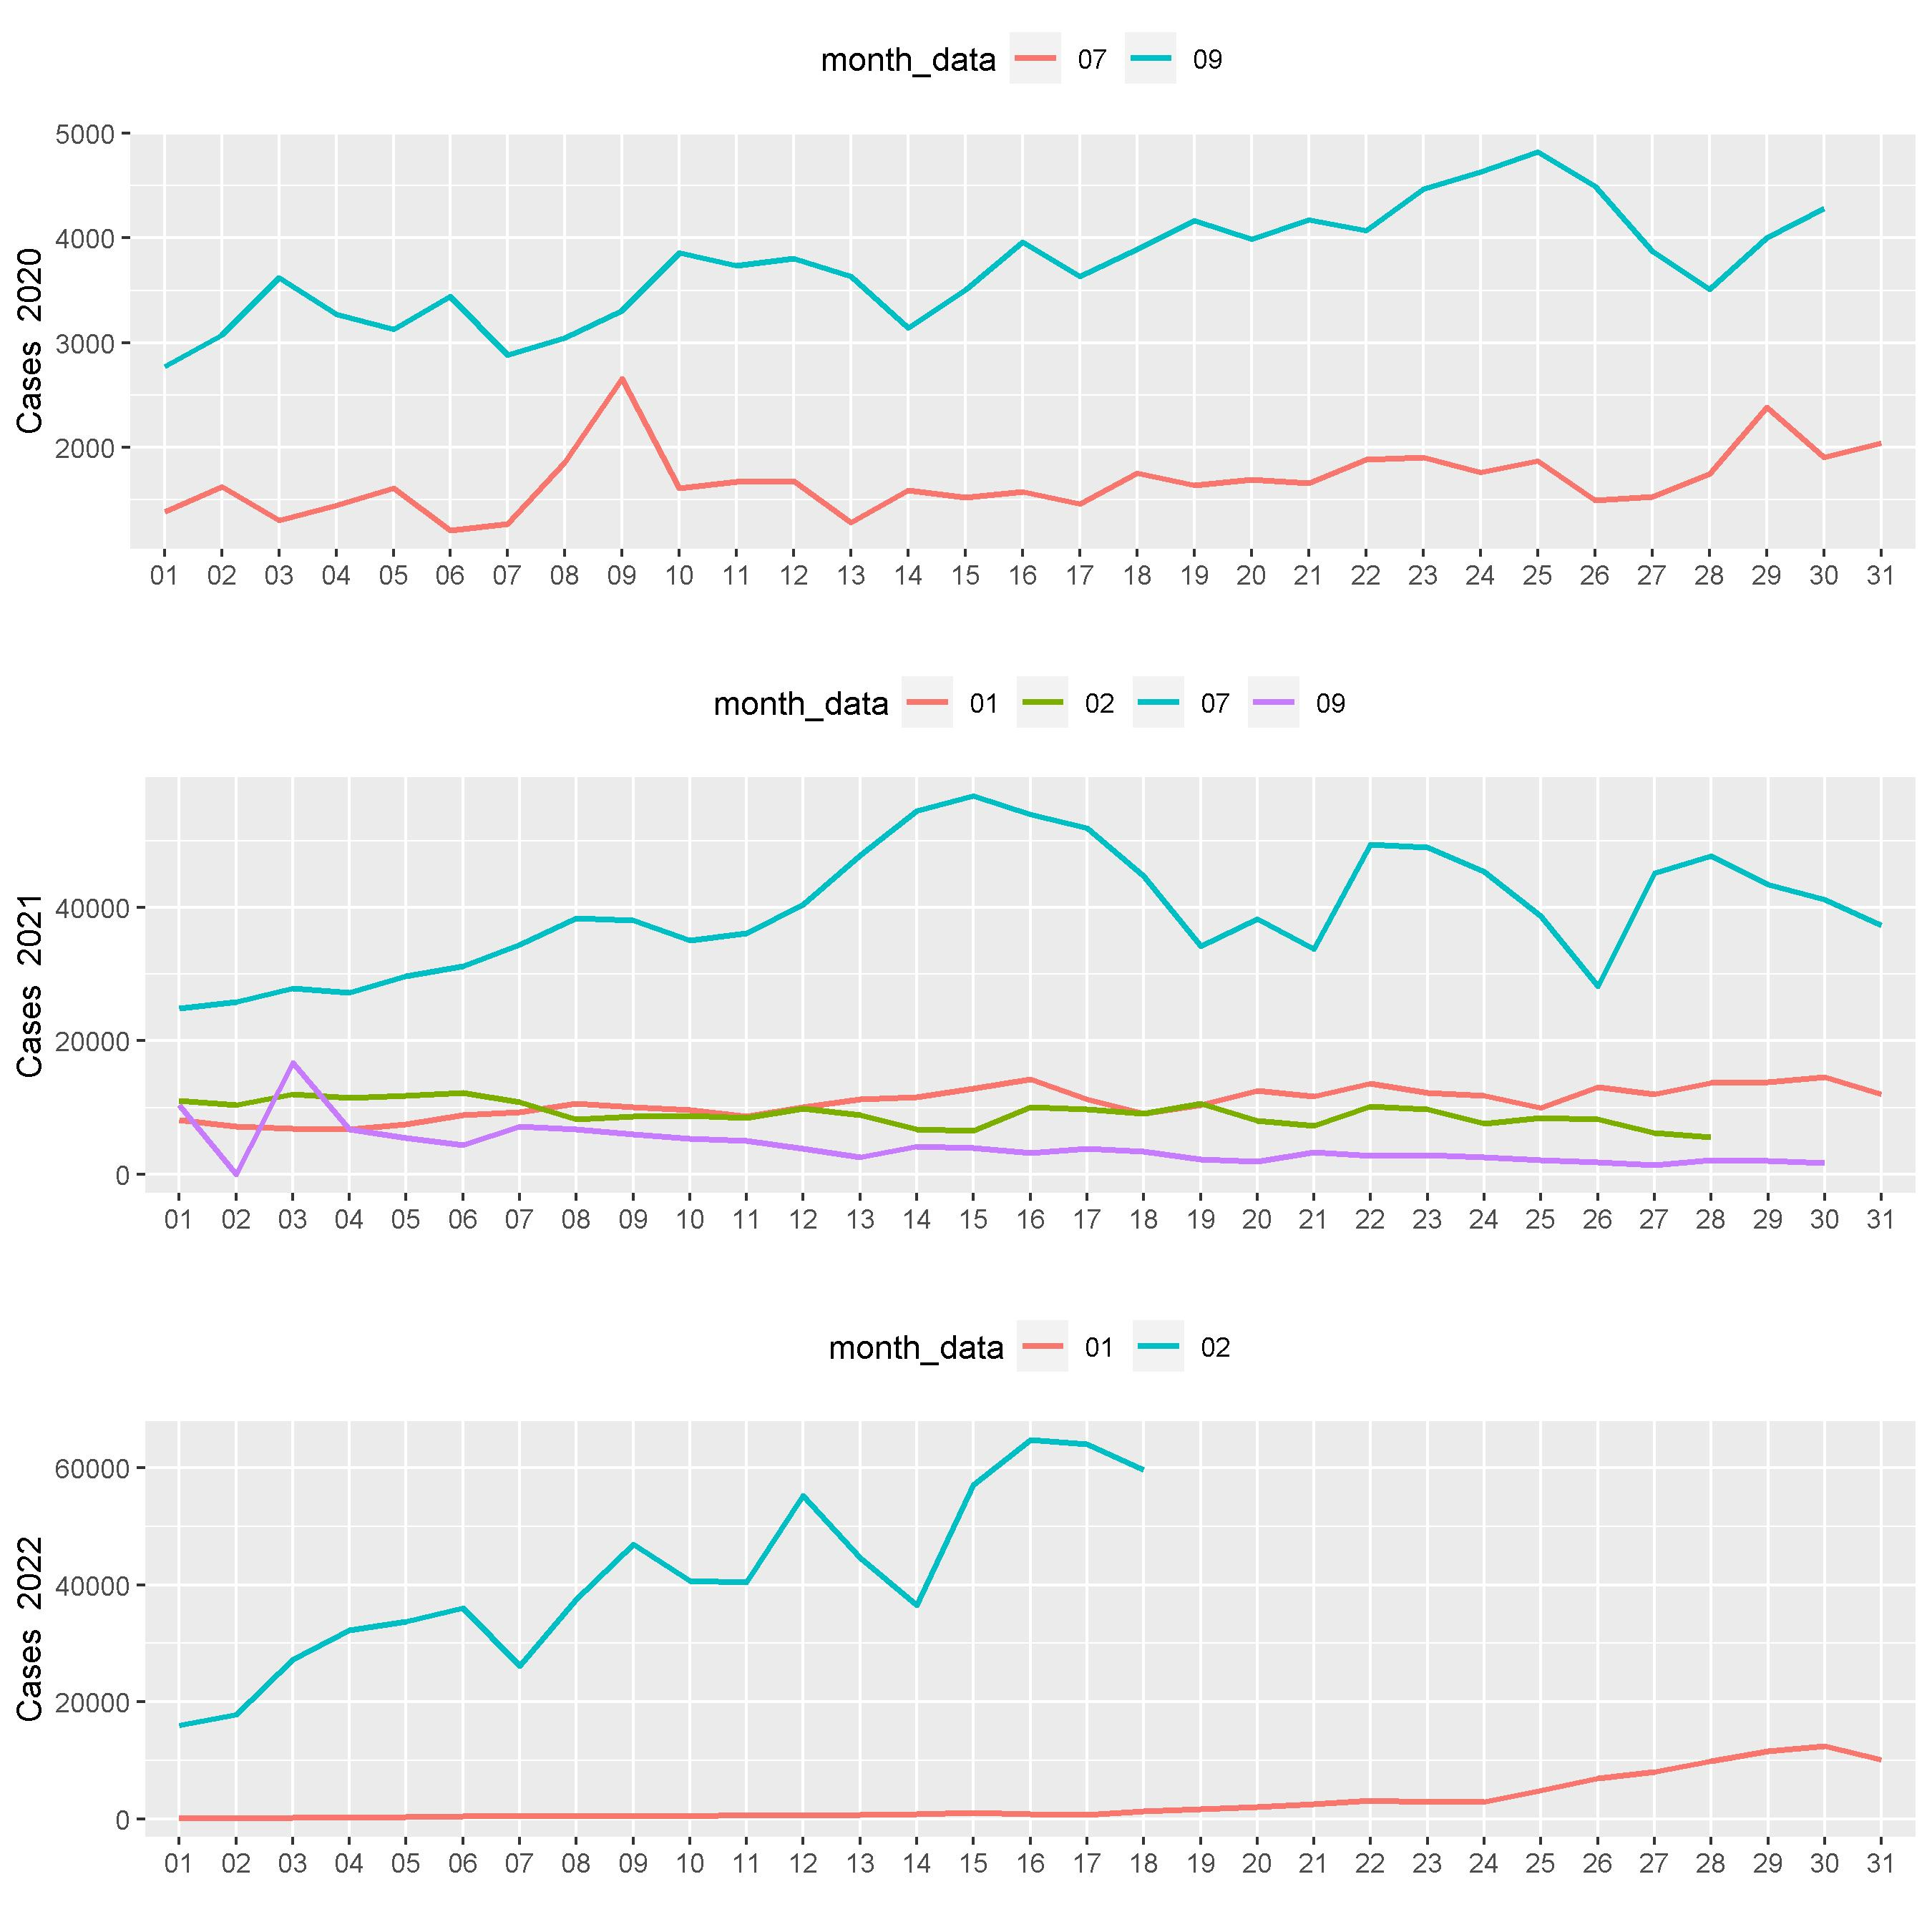
\includegraphics[scale = 0.7]{Images/V/v1 Indonesia .jpeg}
		    \caption{Biểu đồ thể hiện thu thập dữ liệu nhiễm bệnh của Indonesia}
		    \label{fig:my_label}
		\end{figure}
		\begin{figure}[htp]
		    \centering
		    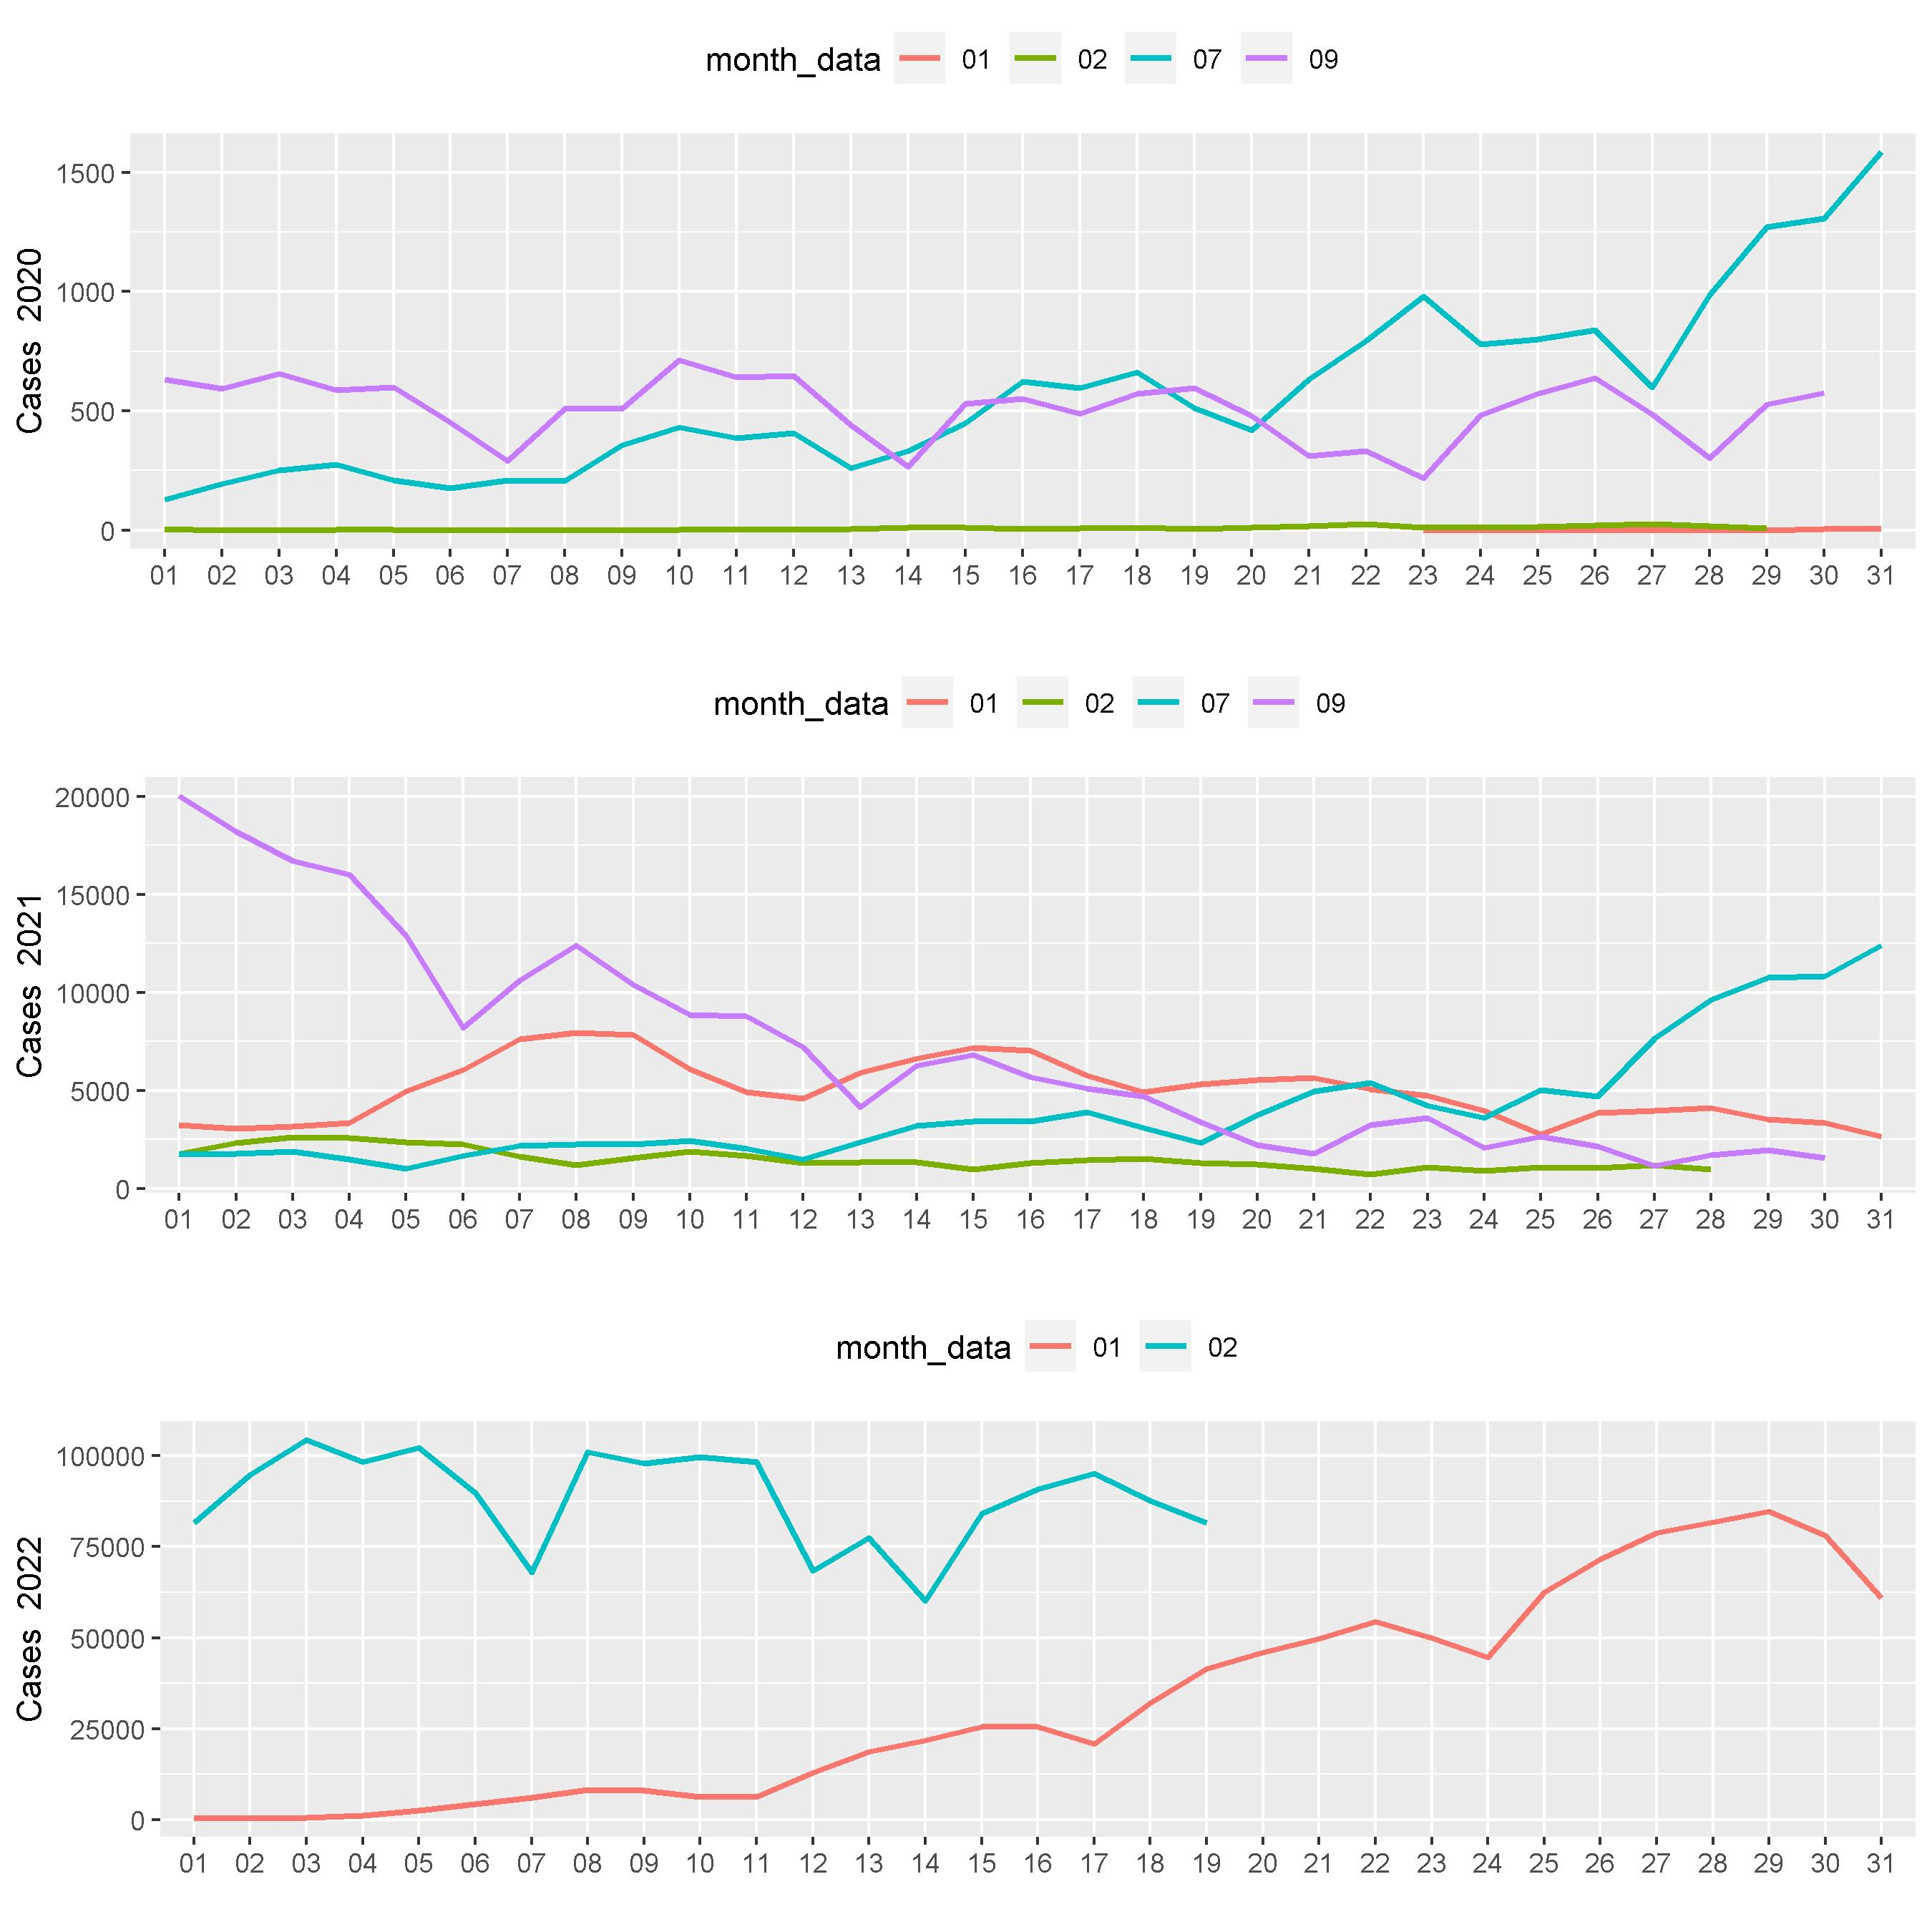
\includegraphics[scale = 0.7]{Images/V/v1 Japan .jpeg}
		    \caption{Biểu đồ thể hiện thu thập dữ liệu nhiễm bệnh của Nhật Bản}
		    \label{fig:my_label}
		\end{figure}
		\begin{figure}[htp]
		    \centering
		    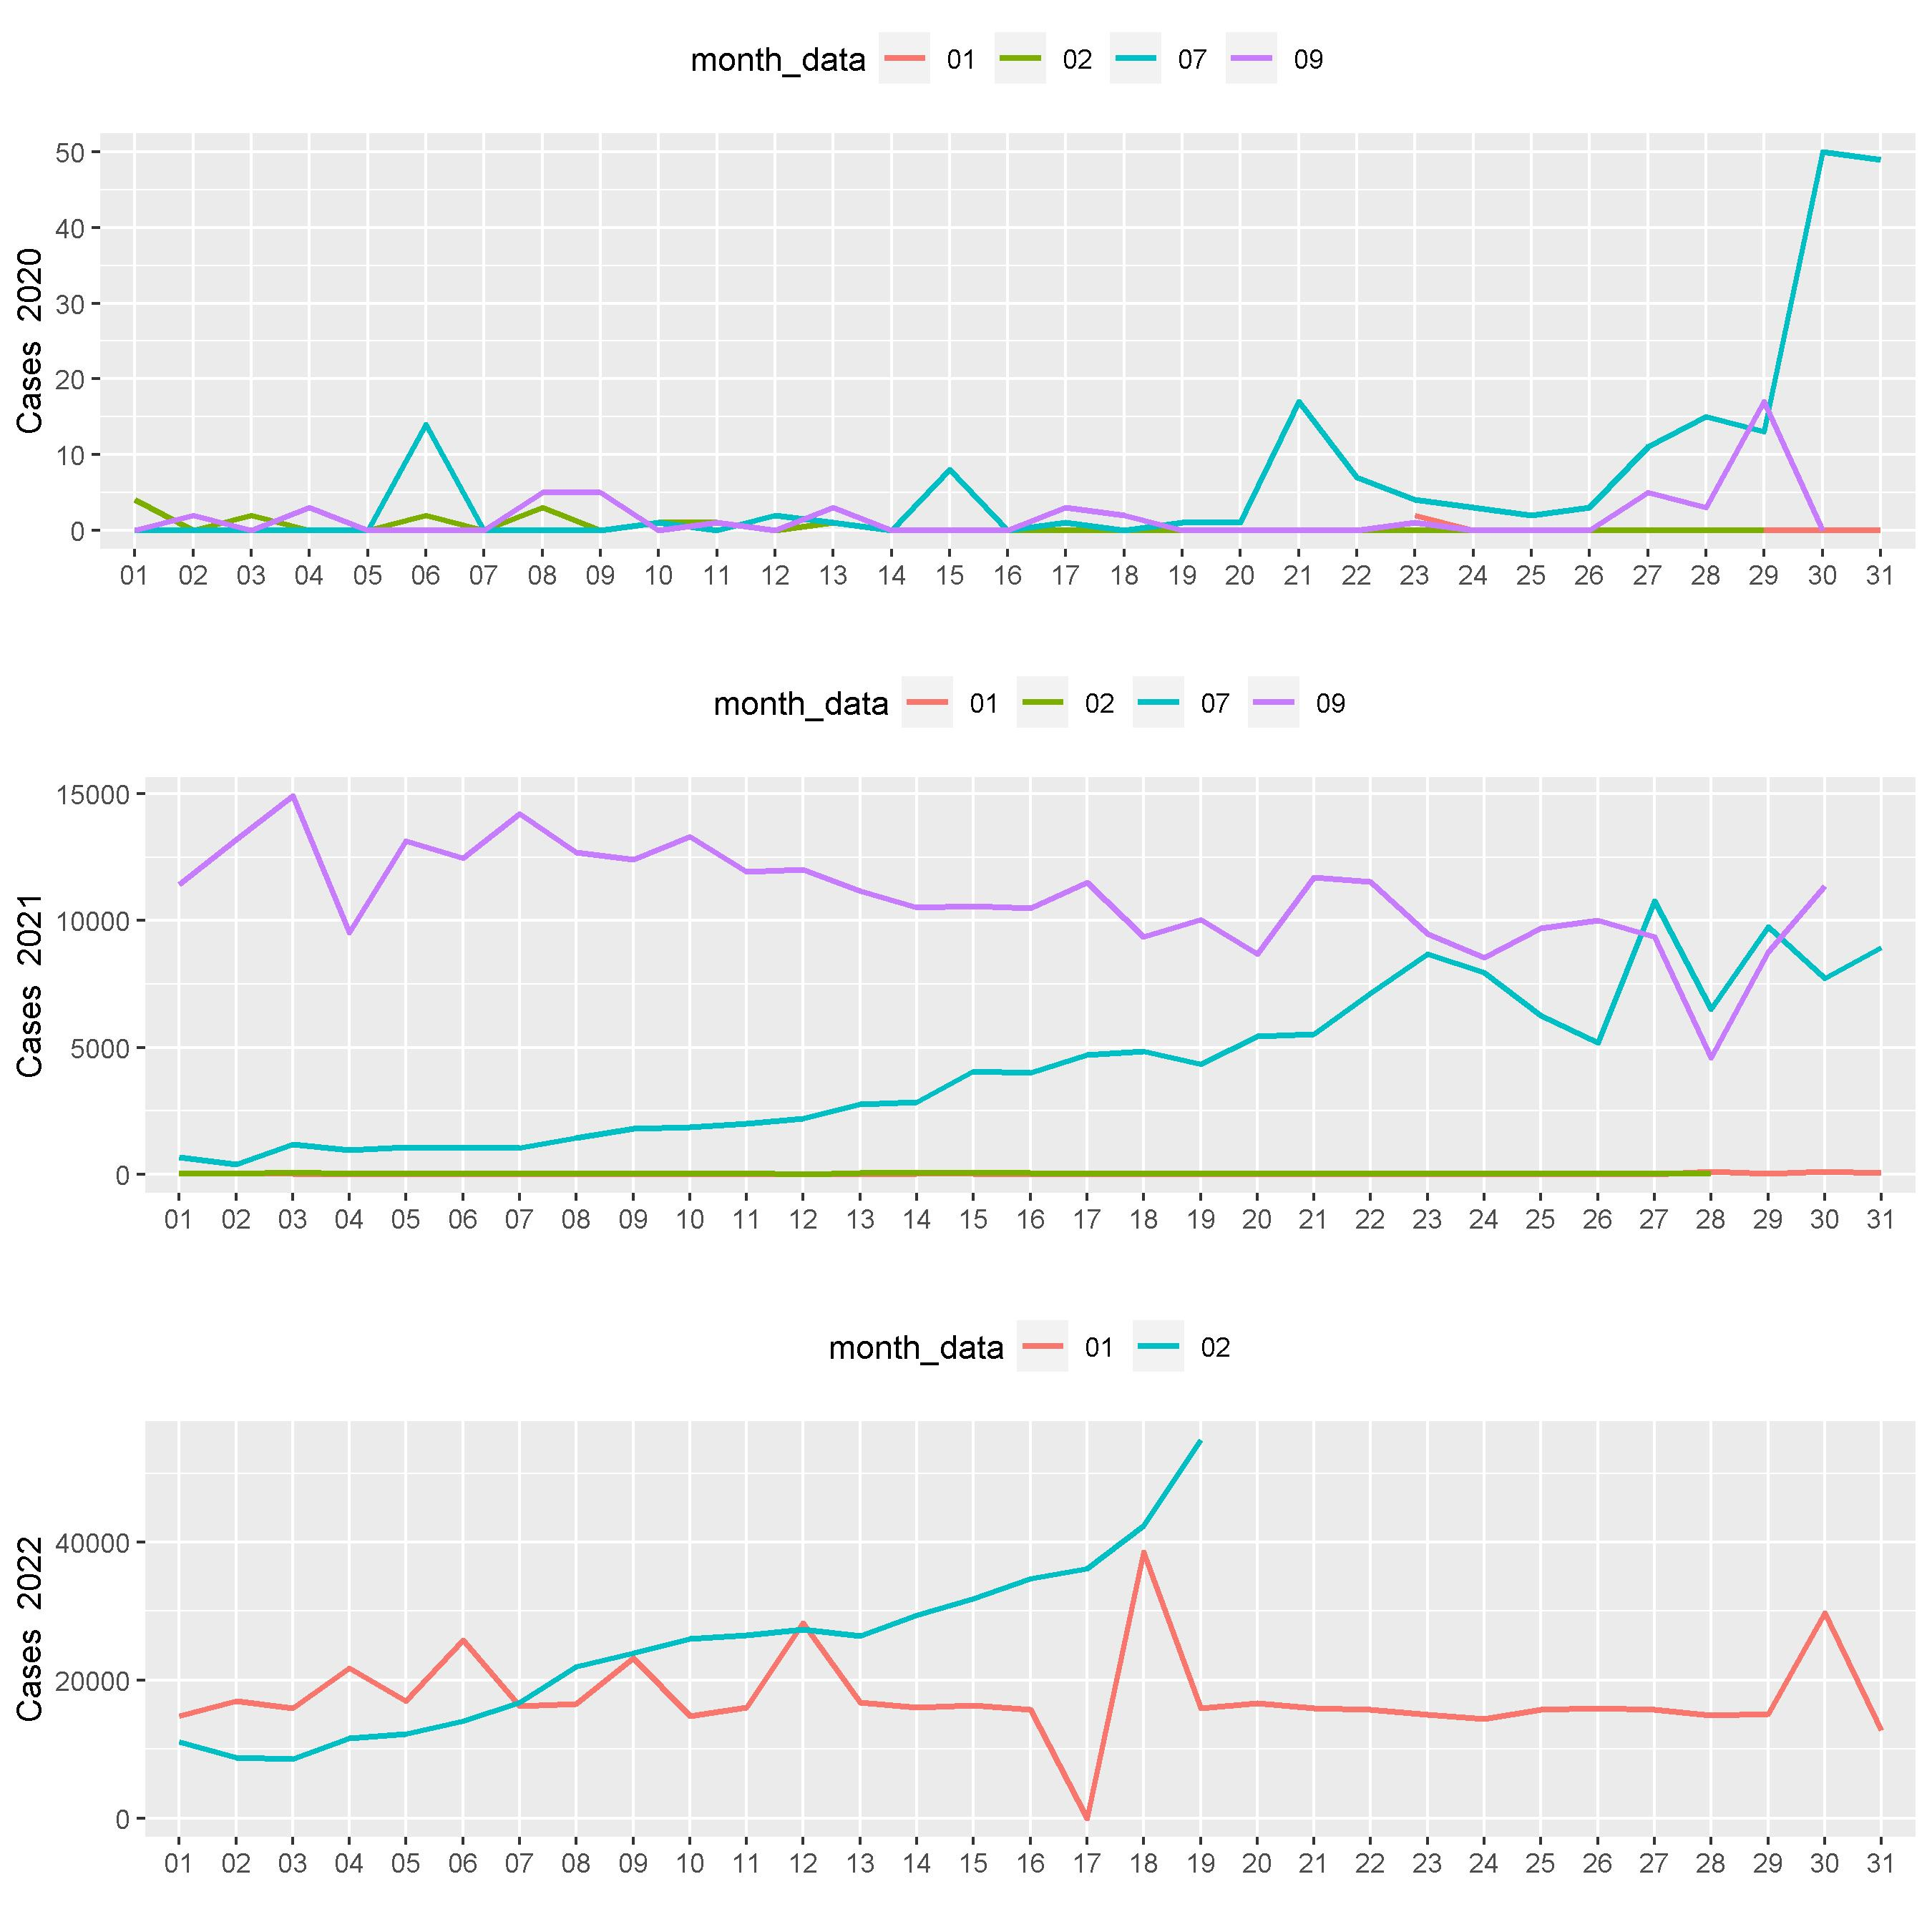
\includegraphics[scale = 0.7]{Images/V/v1 Vietnam .jpeg}
		    \caption{Biểu đồ thể hiện thu thập dữ liệu nhiễm bệnh của Việt Nam}
		    \label{fig:my_label}
		\end{figure}
	%%%%%%%%%%%v2%%%%%%%%%	
	\newpage
    \item Biểu đồ thể hiện thu thập dữ liệu tử vong cho từng tháng
    	\begin{lstlisting}[frame=single]  
#v2
country_chart("Vietnam","line_chart","2_1_7_9","deaths","v2")
country_chart("Japan","line_chart","2_1_7_9","deaths","v2")
country_chart("Indonesia","line_chart","2_1_7_9","deaths","v2")
		\end{lstlisting}	
        \begin{figure}[htp]
		    \centering
		    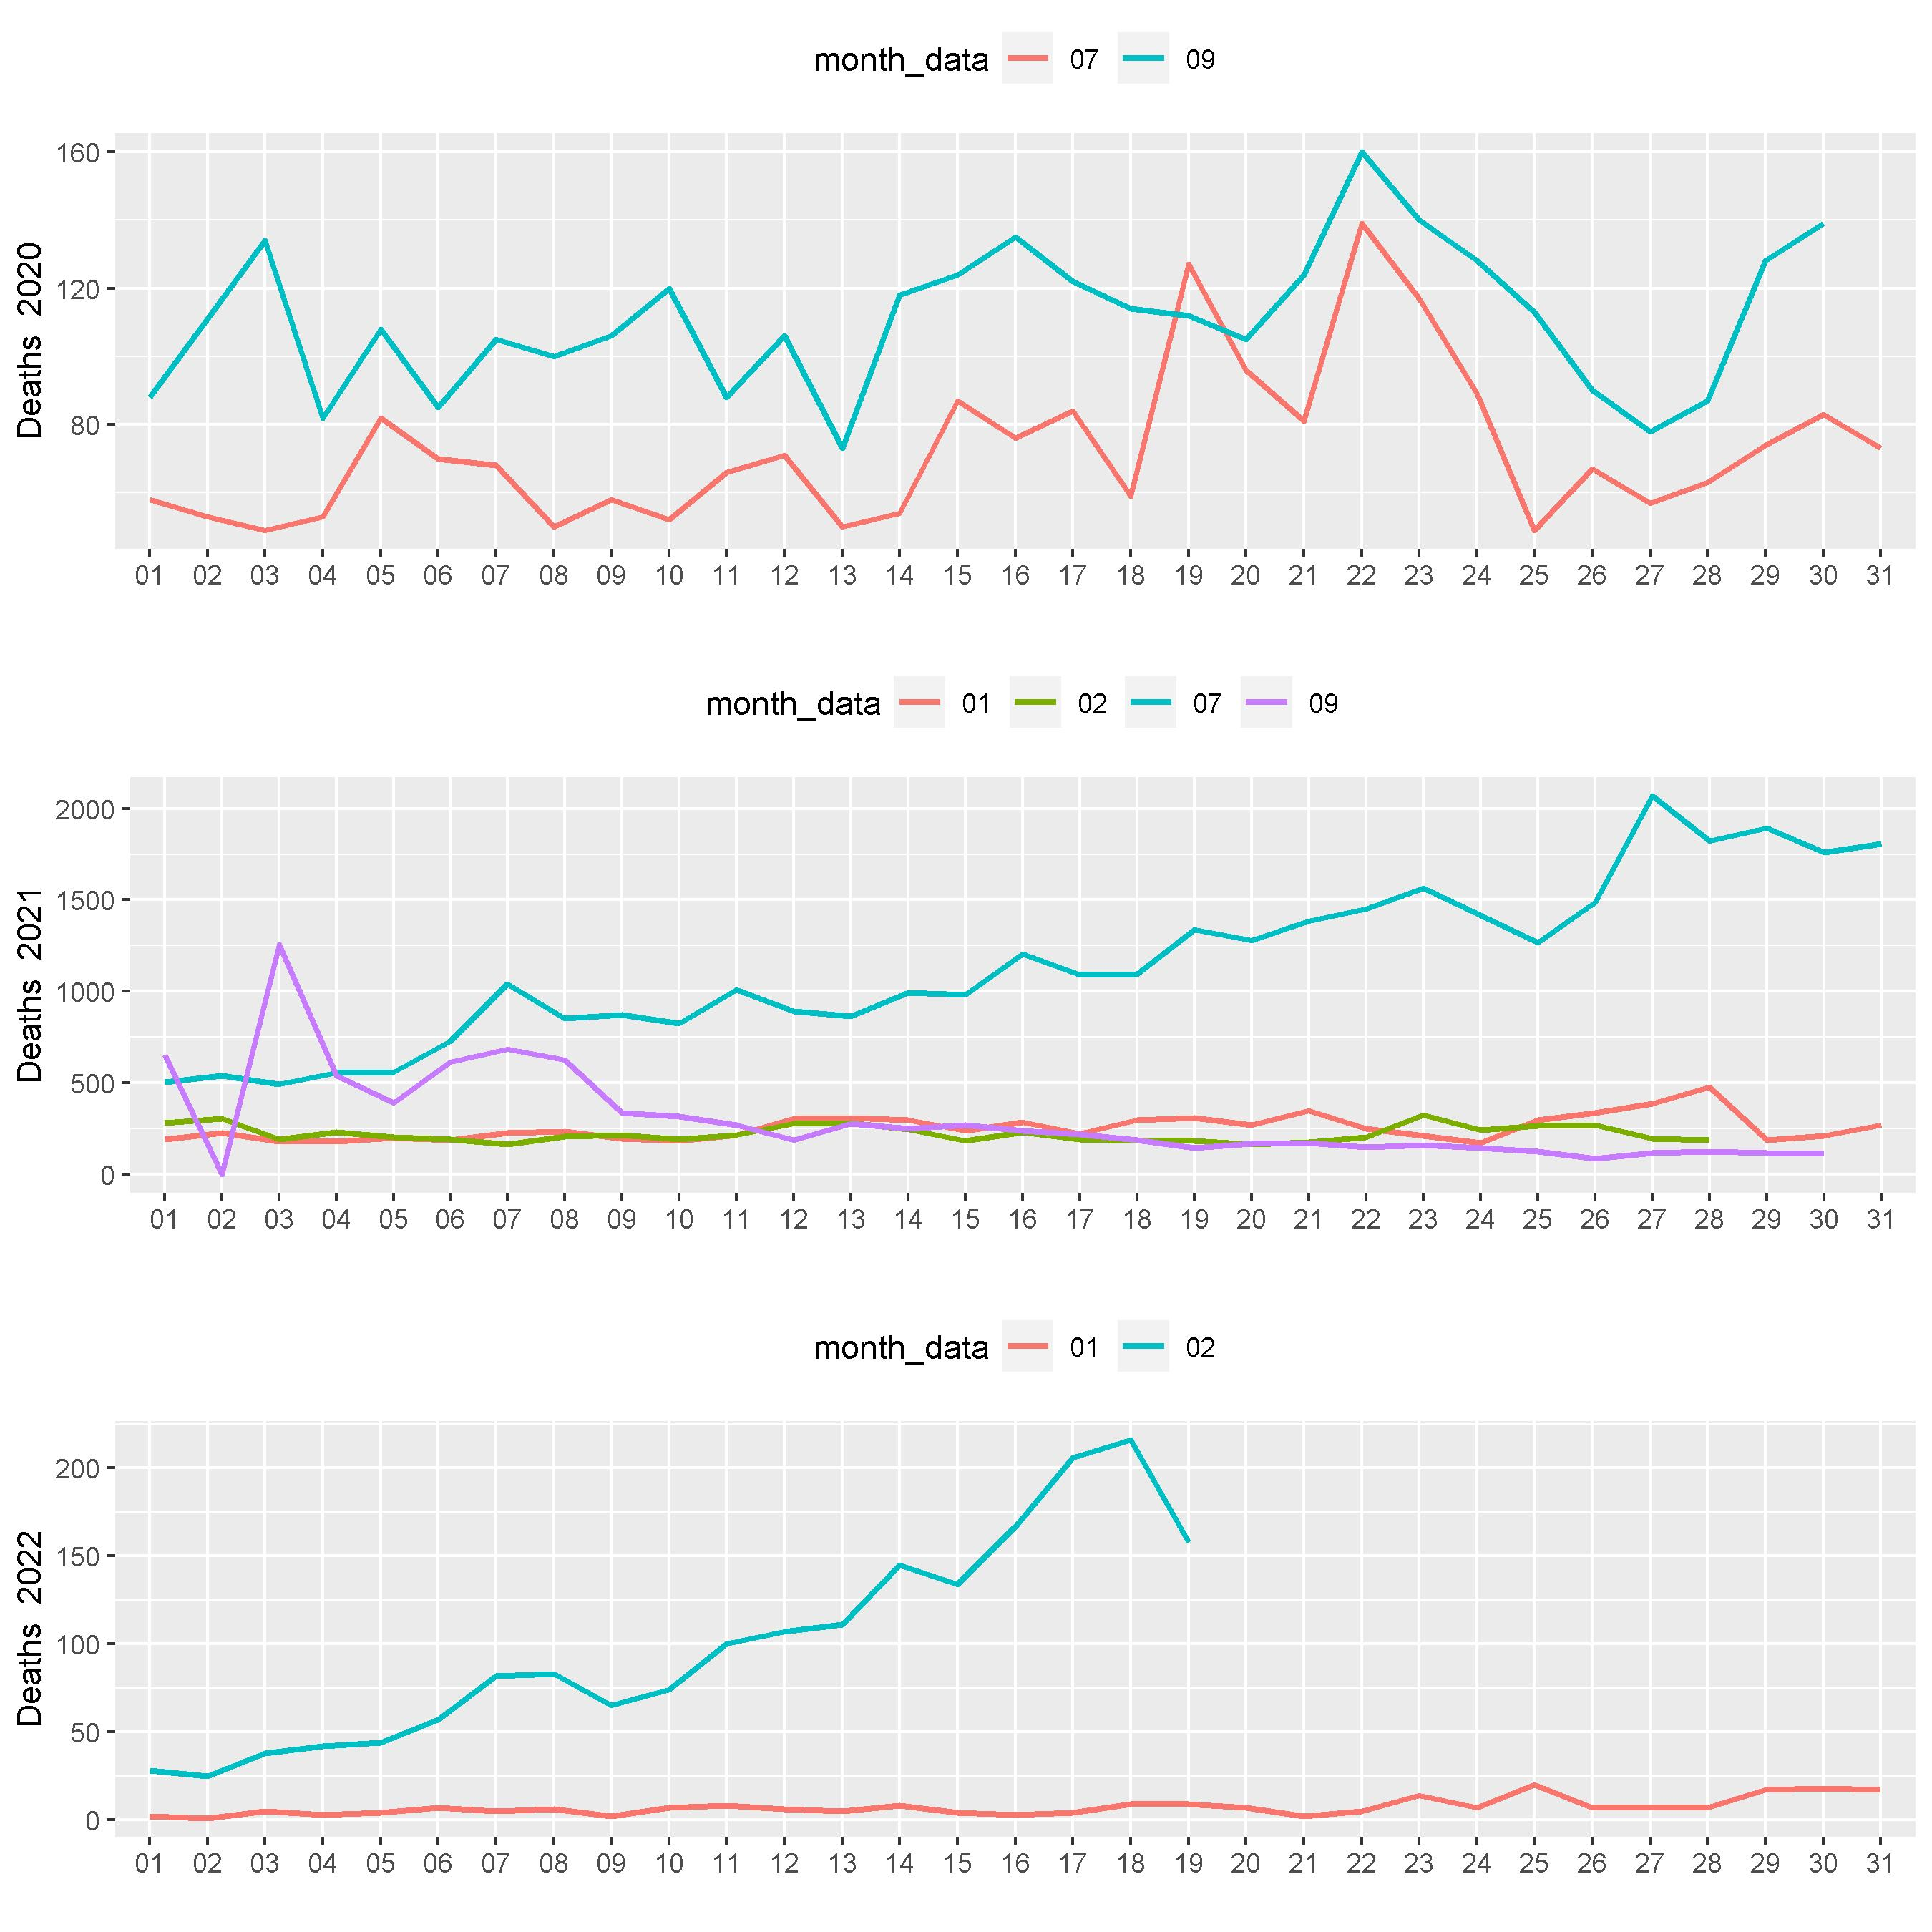
\includegraphics[scale = 0.7]{Images/V/v2 Indonesia .jpeg}
		    \caption{Biểu đồ thể hiện thu thập dữ liệu tử vong của Indonesia}
		    \label{fig:my_label}
		\end{figure}
		\begin{figure}[htp]
		    \centering
		    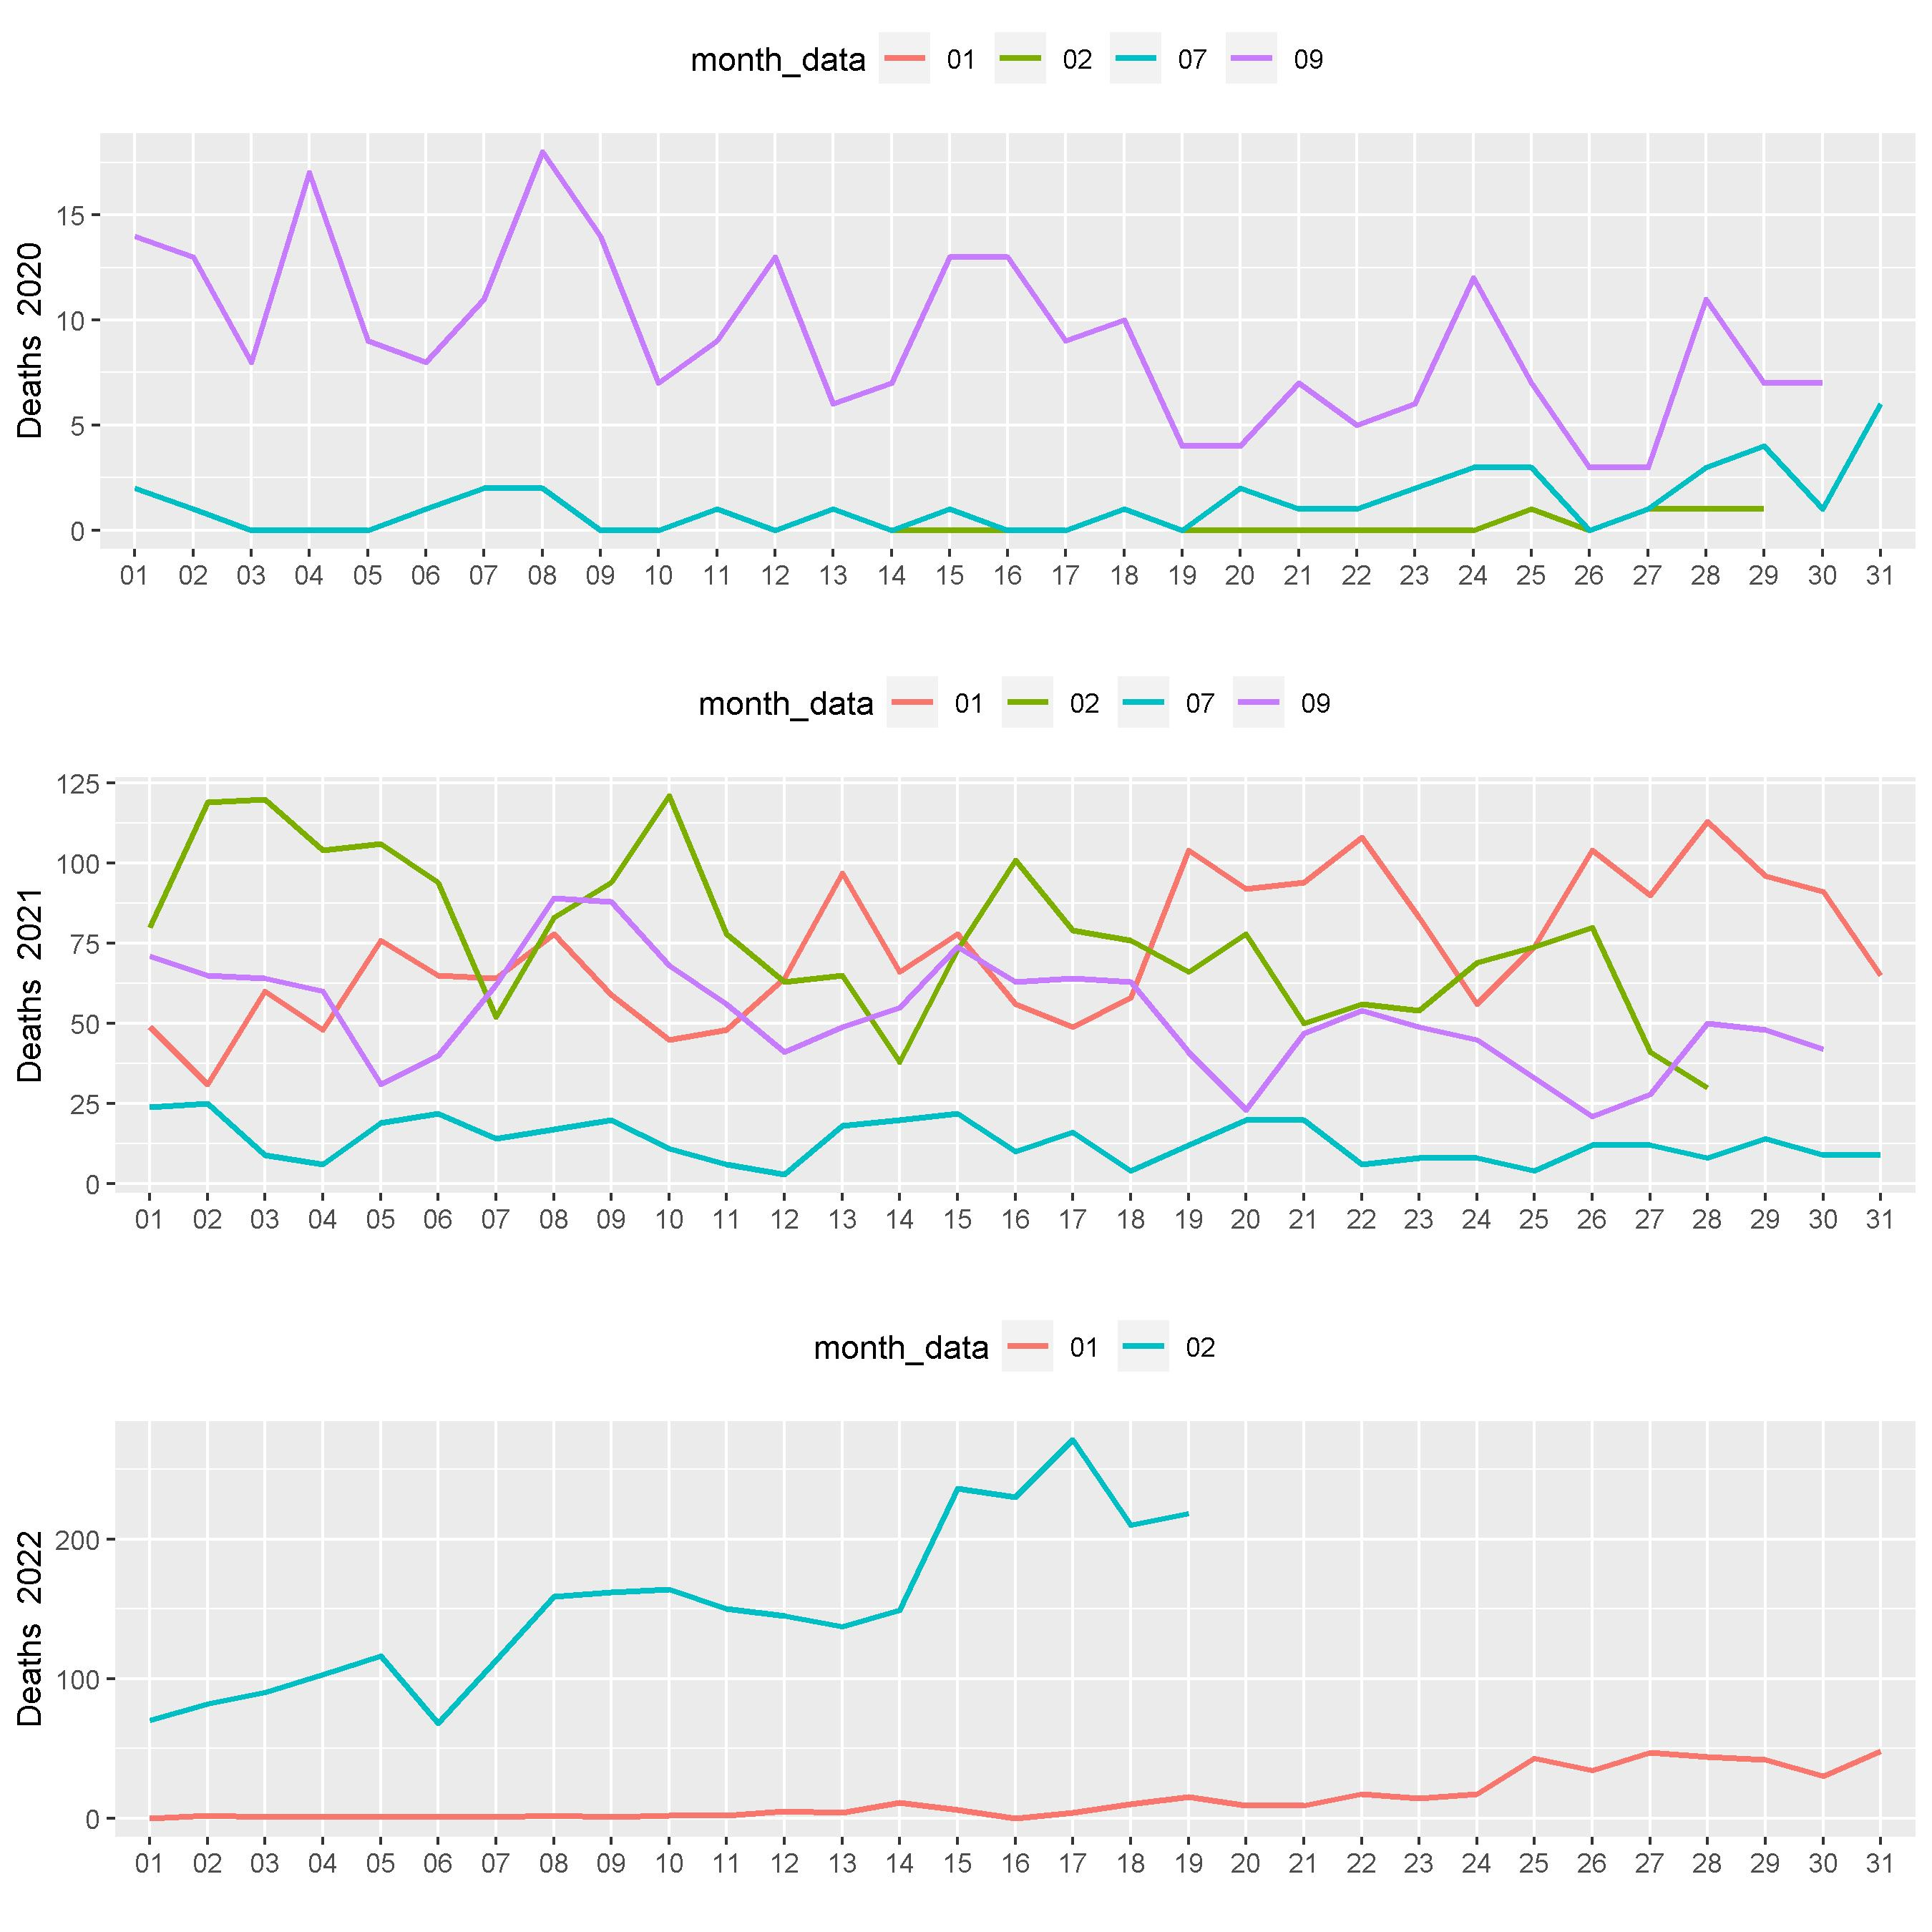
\includegraphics[scale = 0.7]{Images/V/v2 Japan .jpeg}
		    \caption{Biểu đồ thể hiện thu thập dữ liệu tử vong của Nhật Bản}
		    \label{fig:my_label}
		\end{figure}
		\begin{figure}[htp]
		    \centering
		    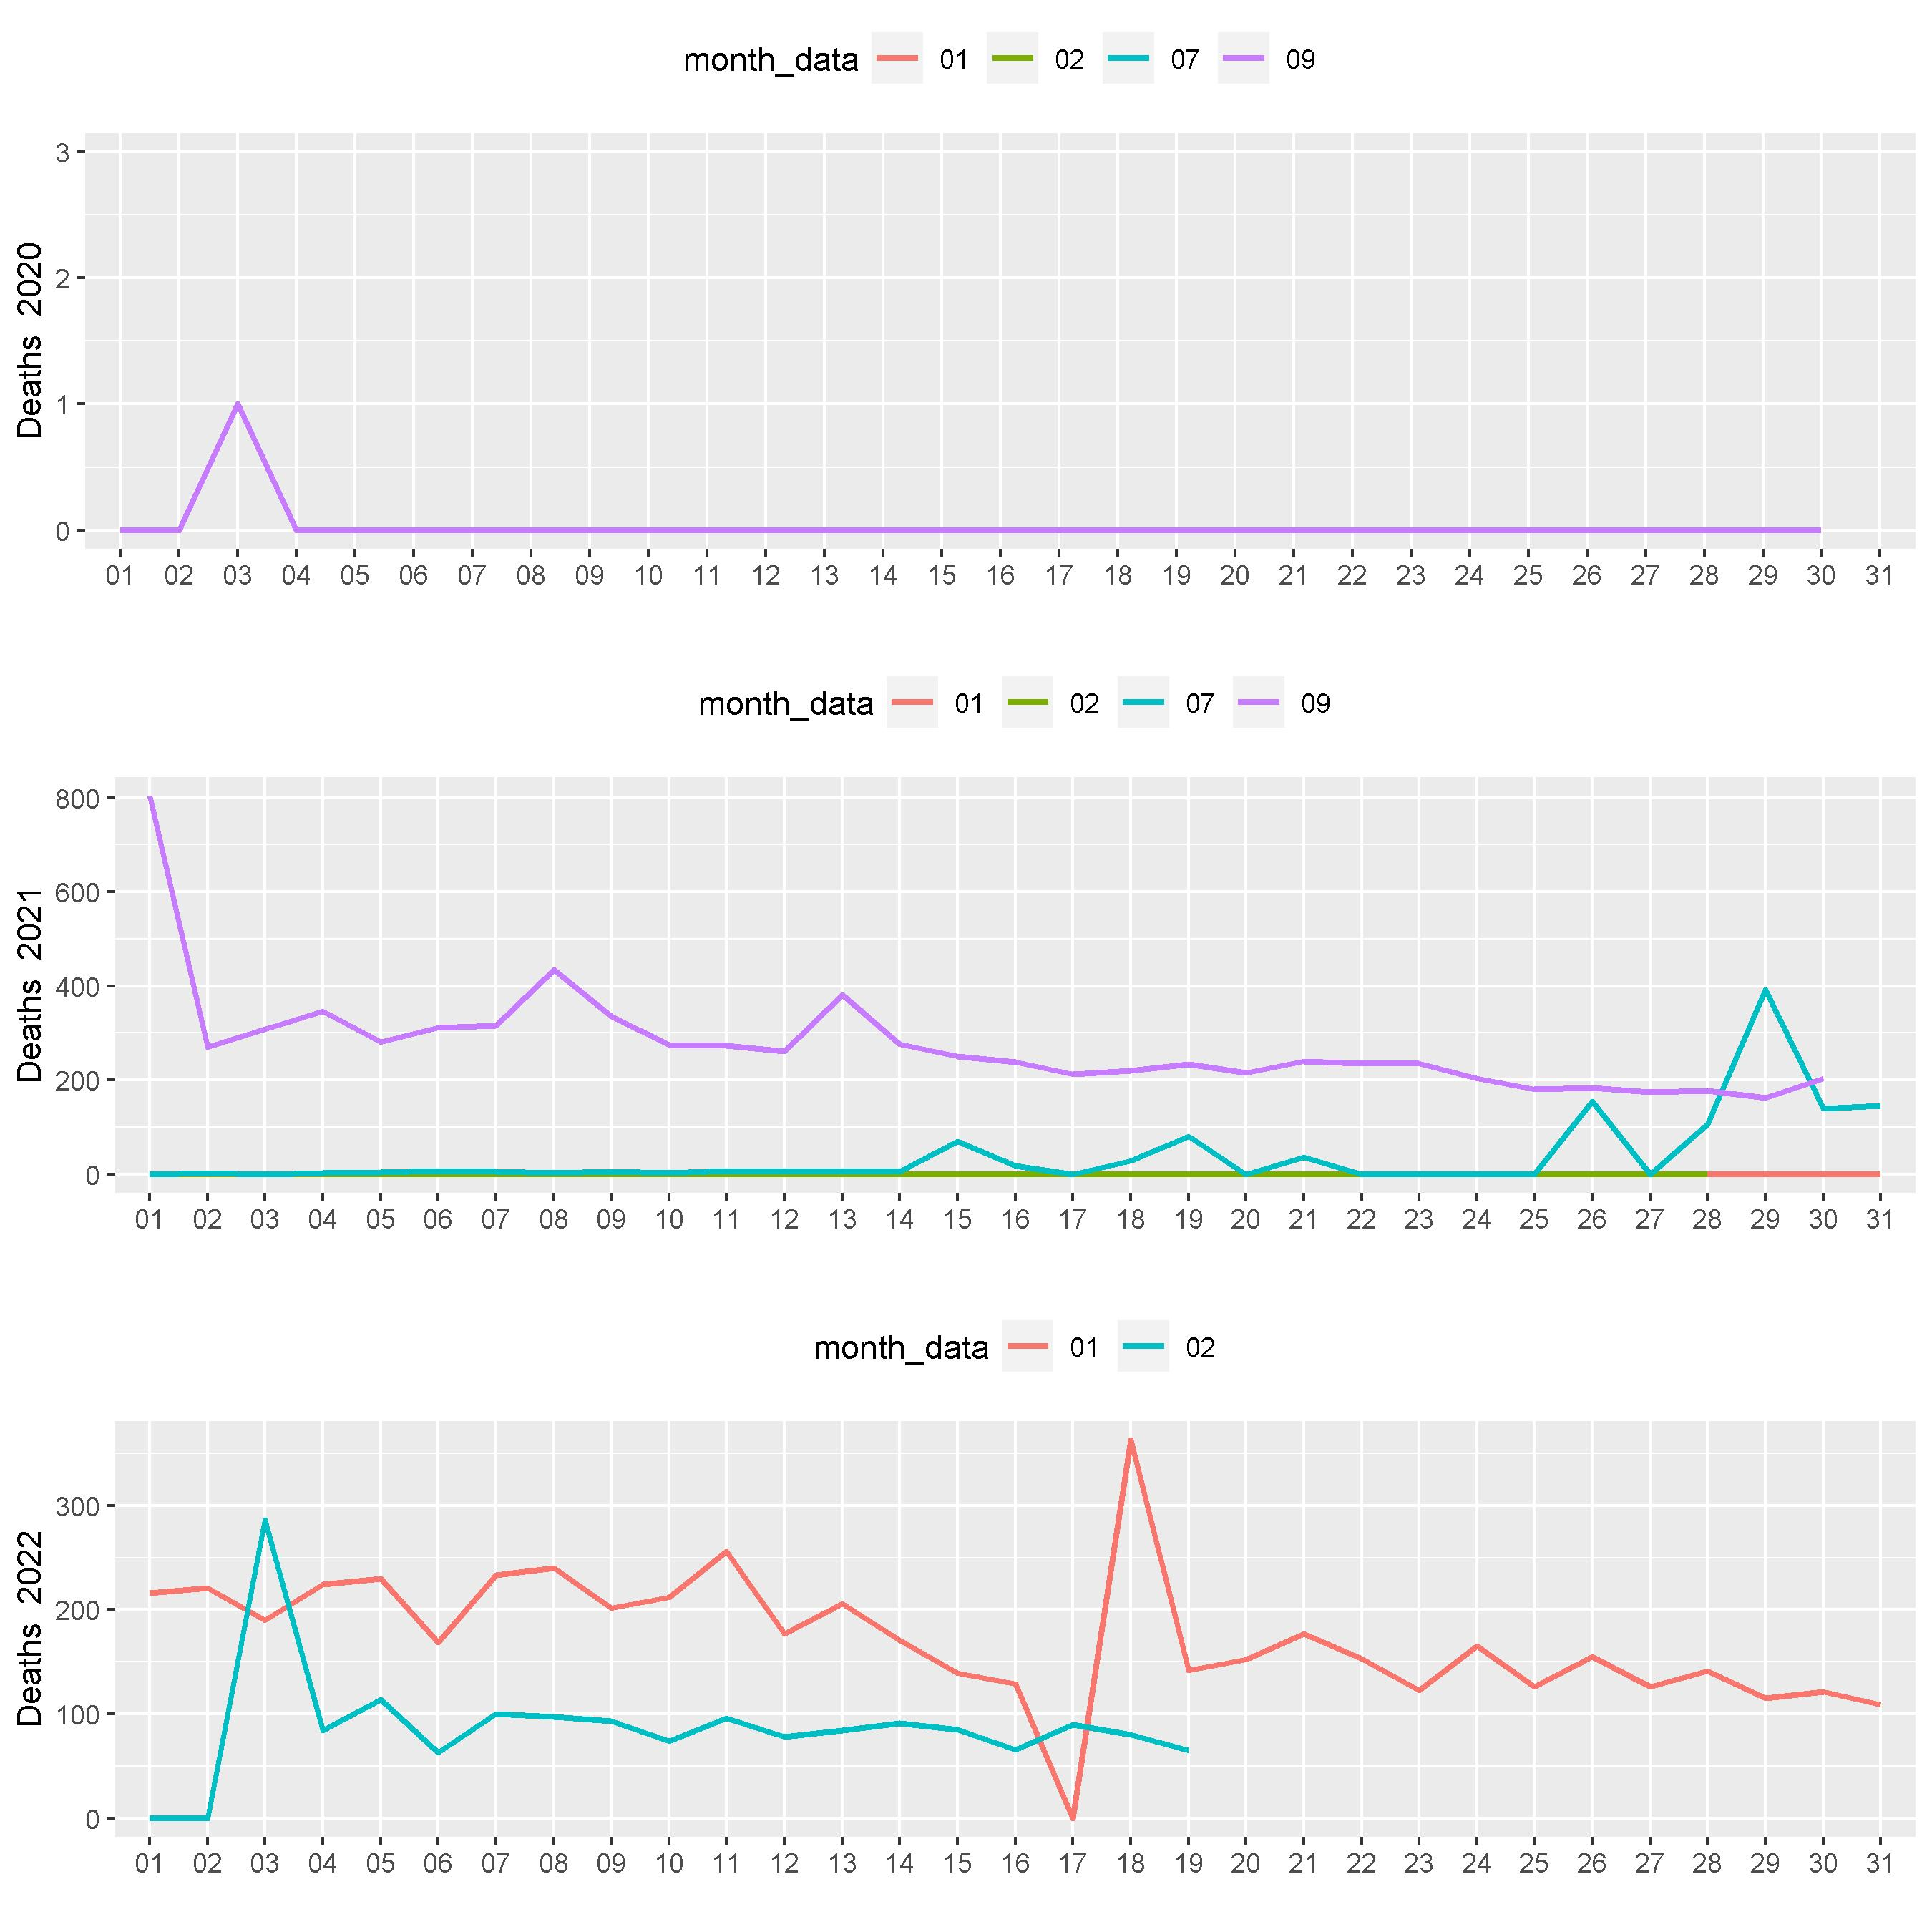
\includegraphics[scale = 0.7]{Images/V/v2 Vietnam .jpeg}
		    \caption{Biểu đồ thể hiện thu thập dữ liệu tử vong của Việt Nam}
		    \label{fig:my_label}
		\end{figure}
    %%%%%%%%v3%%%%%%%%
    \newpage
    \item Biểu đồ thể hiện thu thập dữ liệu gồm nhiễm bệnh và tử vong cho từng tháng
    	\begin{lstlisting}[frame=single]  
#v3
country_chart("Vietnam","two_line","2_1_7_9","","v3")
country_chart("Japan","two_line","2_1_7_9","","v3")
country_chart("Indonesia","two_line","2_1_7_9","","v3")
		\end{lstlisting}	
		\begin{figure}[htp]
		    \centering
		    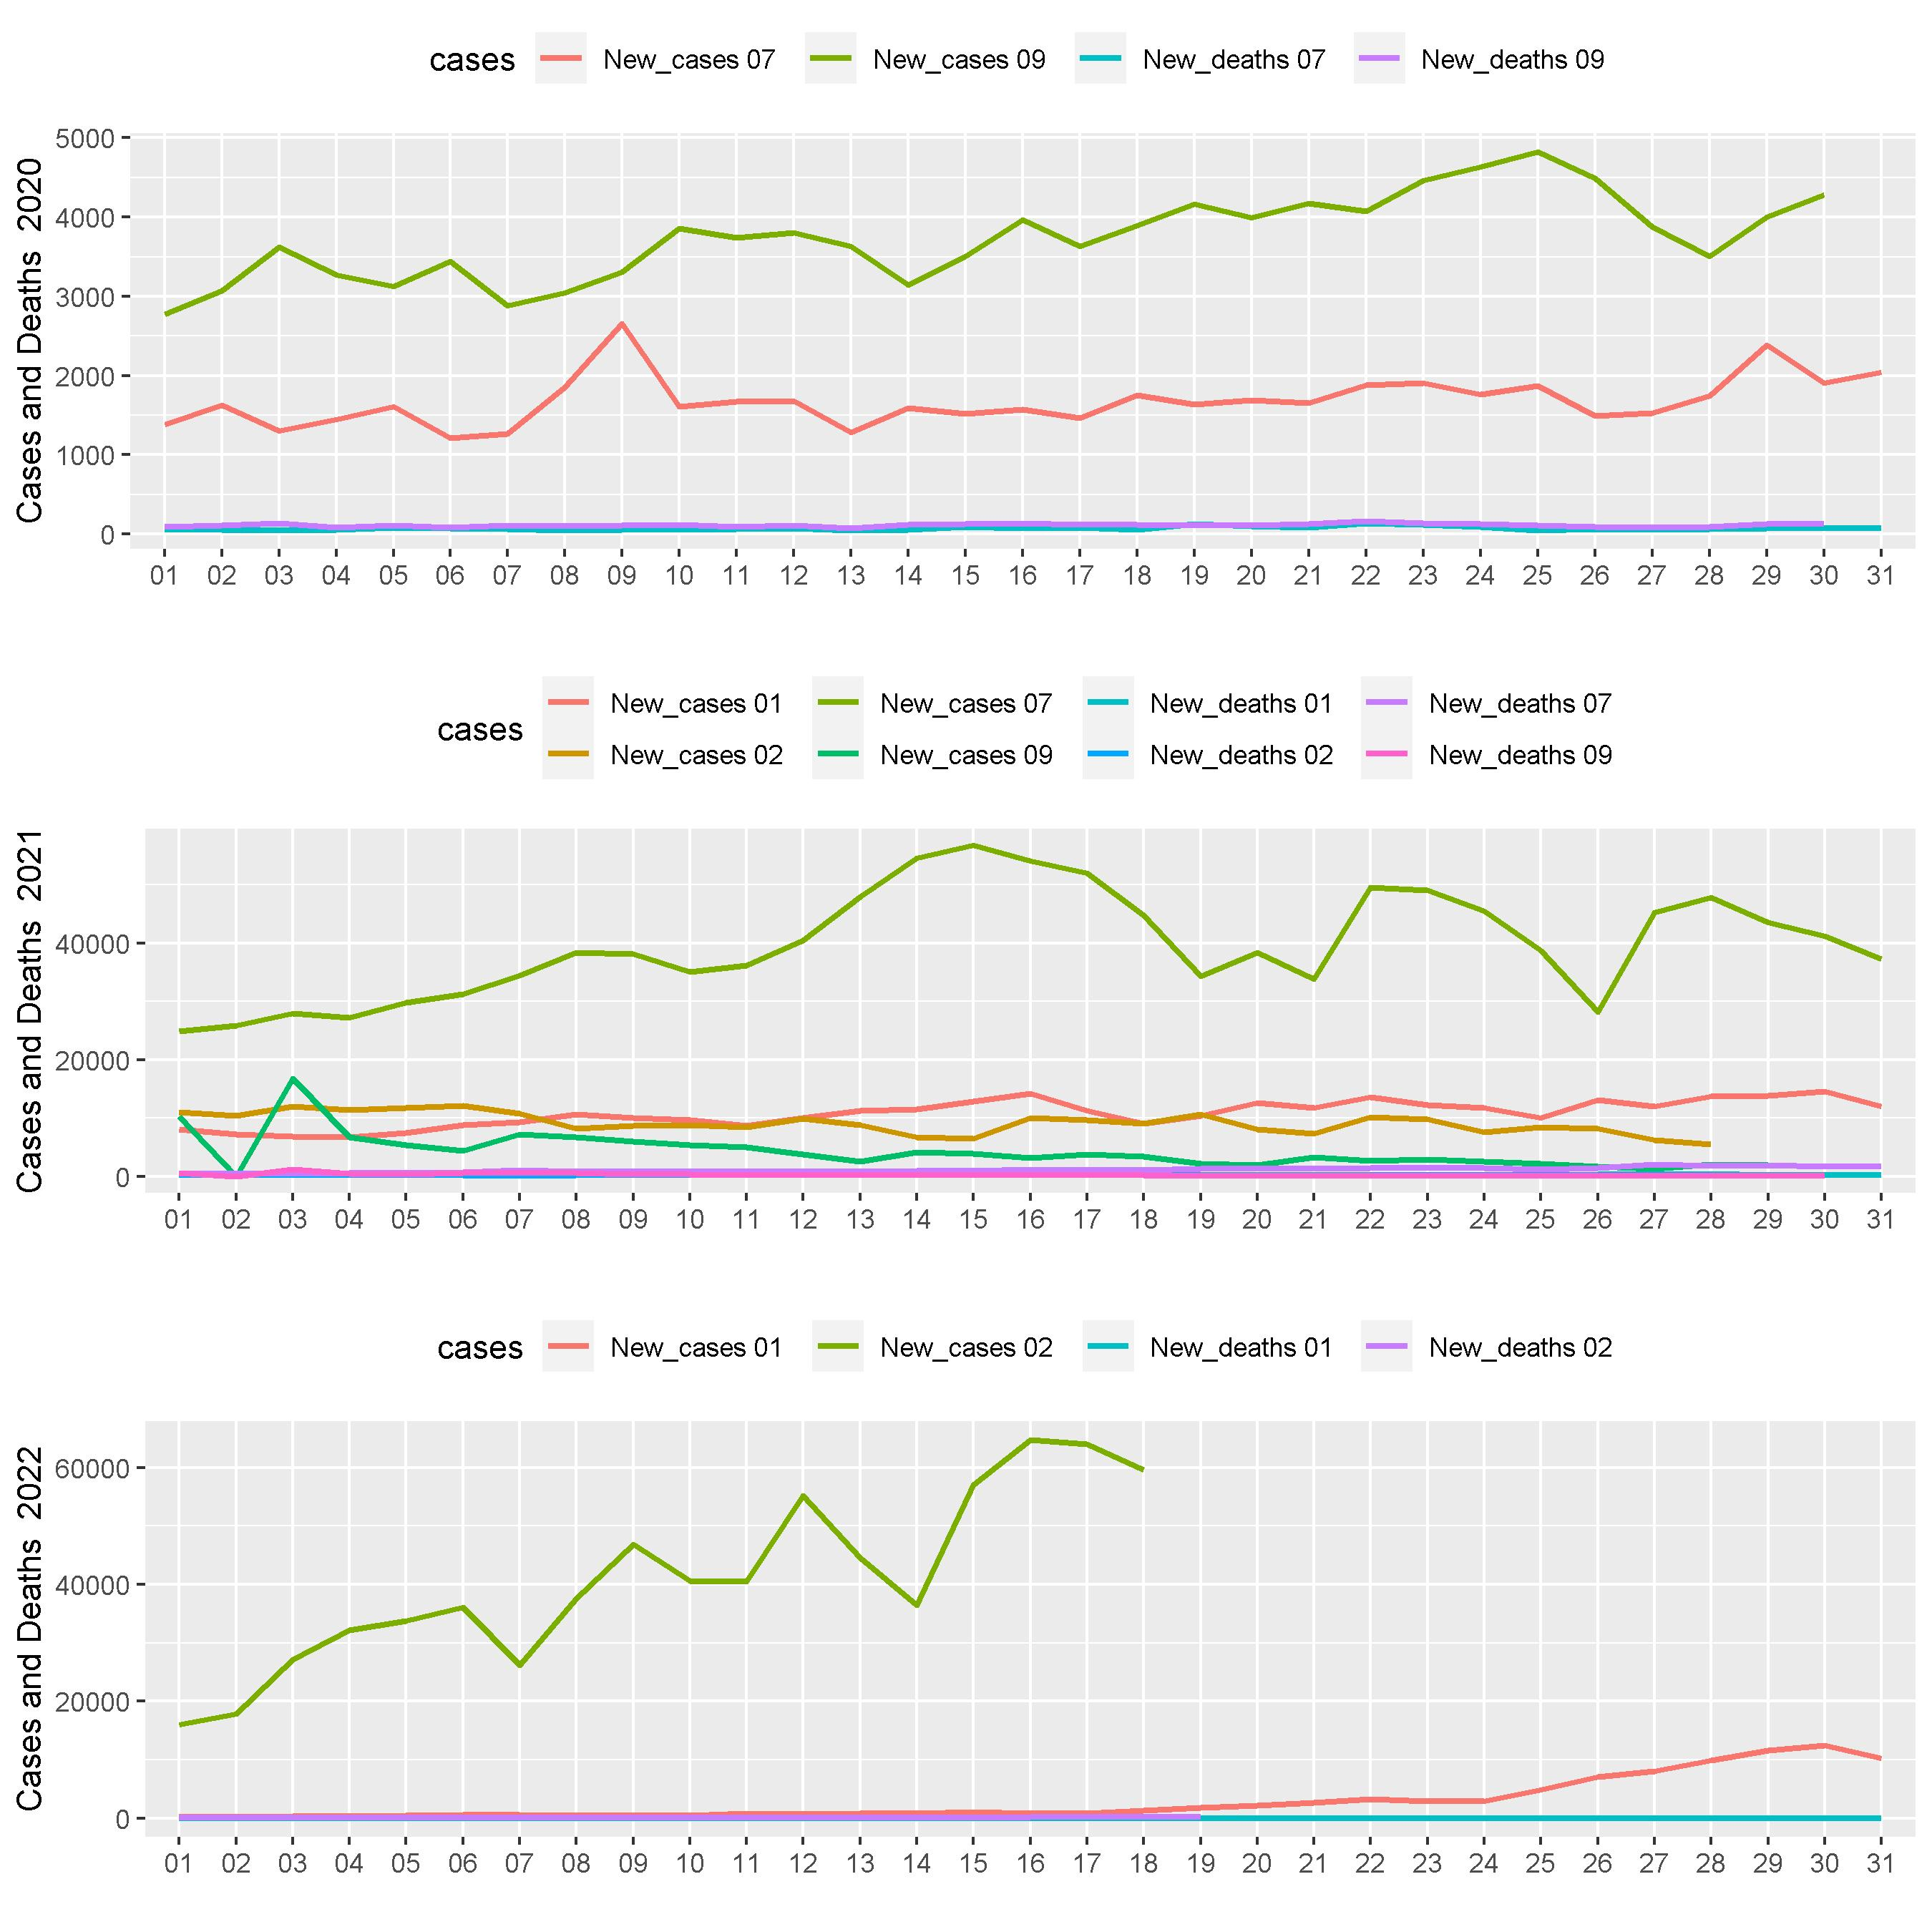
\includegraphics[scale = 0.7]{Images/V/v3 Indonesia .jpeg}
		    \caption{Biểu đồ thể hiện thu thập dữ liệu nhiễm bệnh và tử vong của Indonesia}
		    \label{fig:my_label}
		\end{figure}
		\begin{figure}[htp]
		    \centering
		    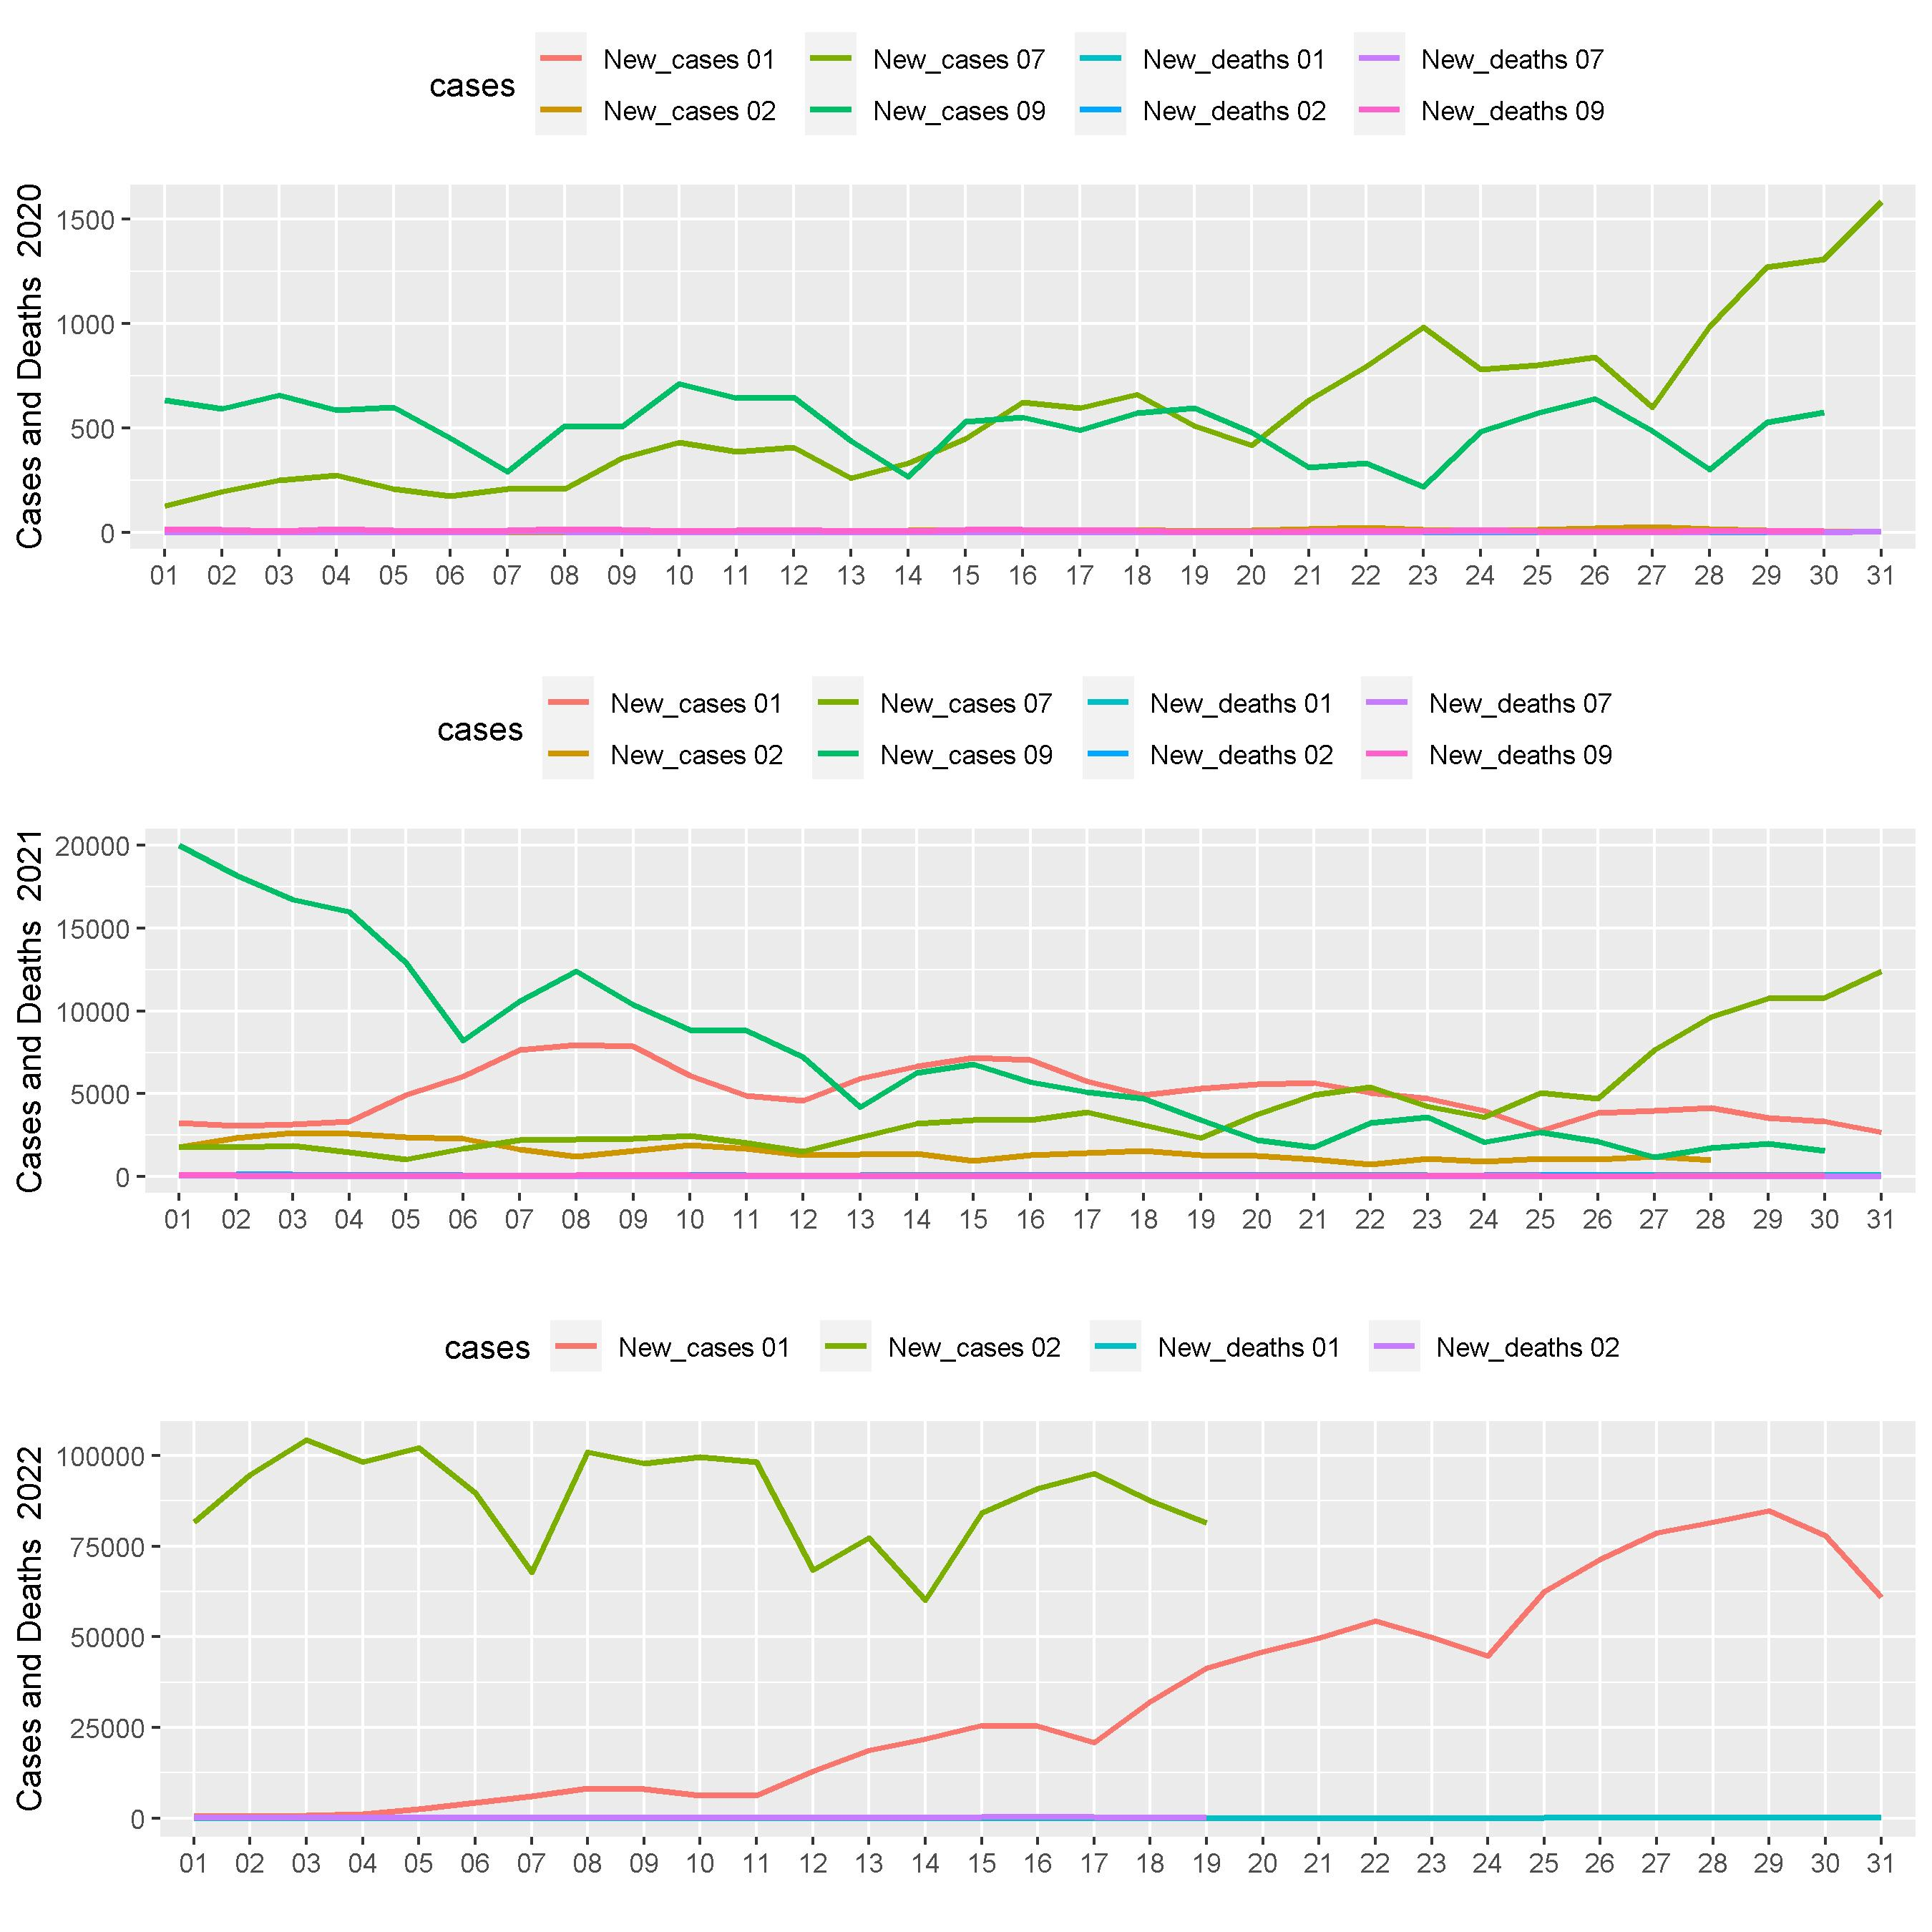
\includegraphics[scale = 0.7]{Images/V/v3 Japan .jpeg}
		    \caption{Biểu đồ thể hiện thu thập dữ liệu nhiễm bệnh và tử vong của Nhật Bản}
		    \label{fig:my_label}
		\end{figure}
		\begin{figure}[htp]
		    \centering
		    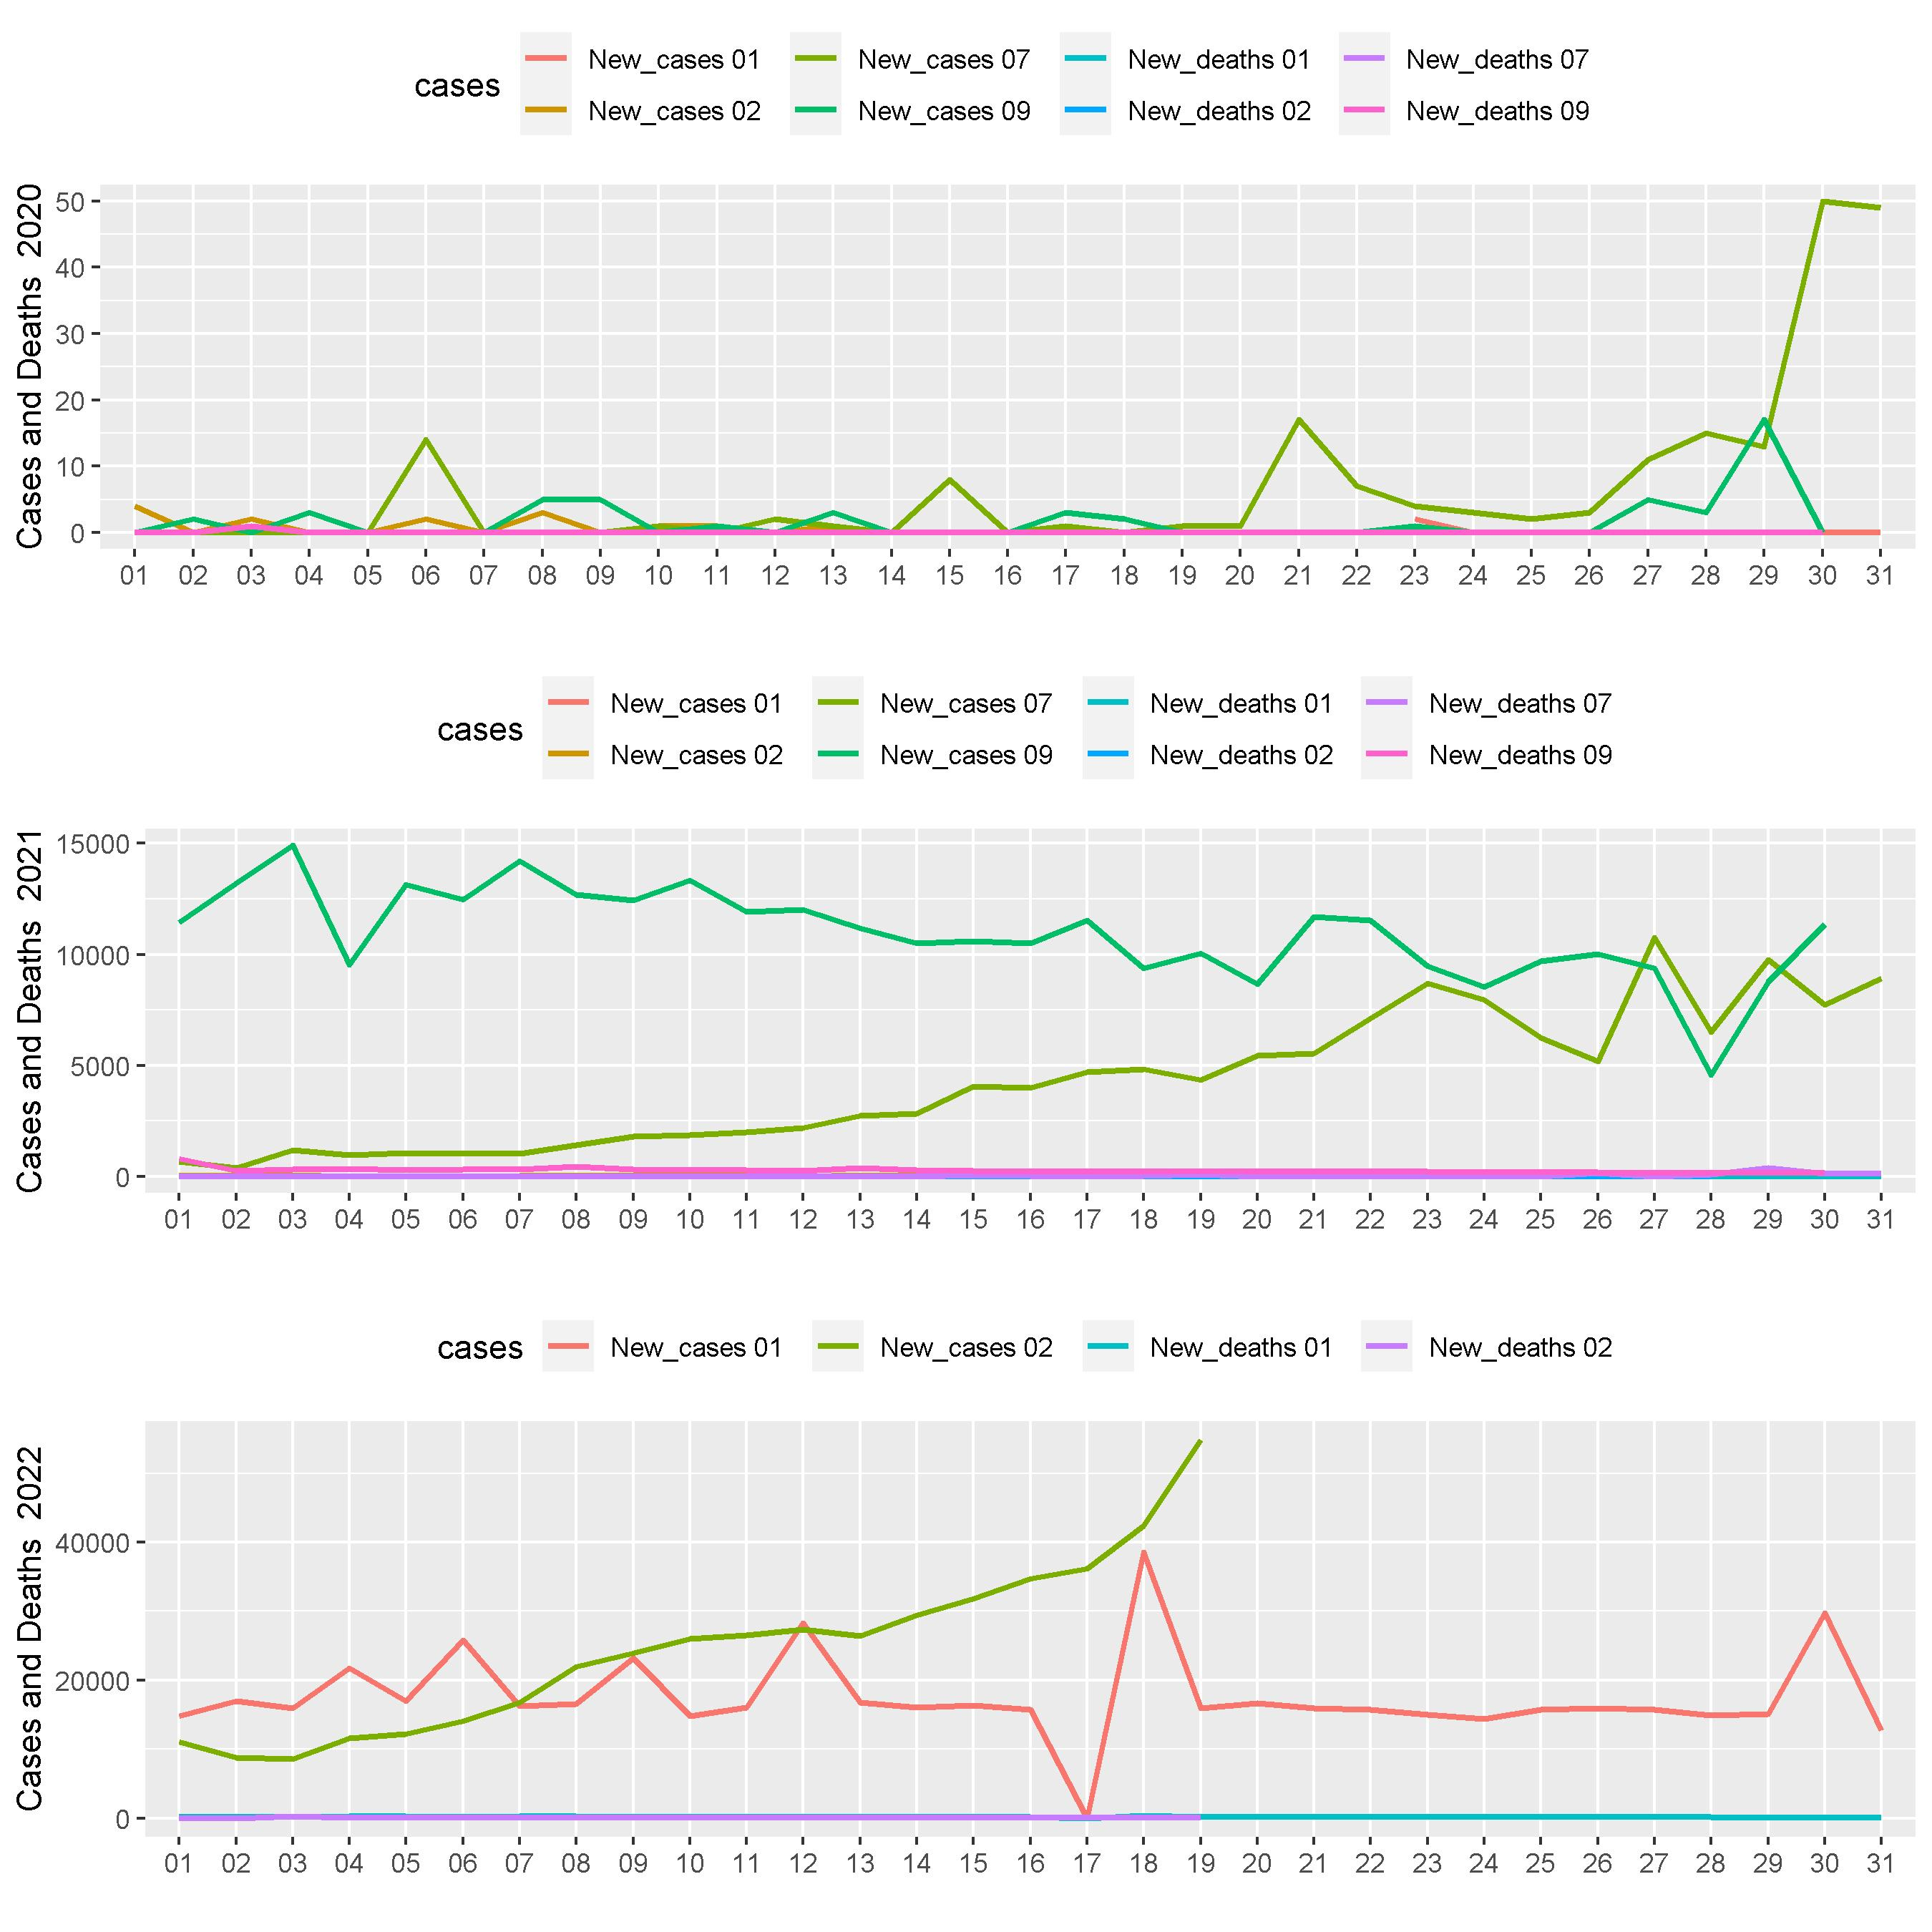
\includegraphics[scale = 0.7]{Images/V/v3 Vietnam .jpeg}
		    \caption{Biểu đồ thể hiện thu thập dữ liệu nhiễm bệnh và tử vong của Việt Nam}
		    \label{fig:my_label}
		\end{figure}
    
    %%%%%%%v4%%%%%%%%%
    \newpage
    \item Biểu đồ thể hiện thu thập dữ liệu nhiễm bệnh gồm 2 tháng cuối của năm
    \begin{lstlisting}[frame=single]  
#v4
country_chart("Vietnam","line_chart","11_12","cases","v4")
country_chart("Japan","line_chart","11_12","cases","v4")
country_chart("Indonesia","line_chart","11_12","cases","v4")
		\end{lstlisting}
		\begin{figure}[htp]
		    \centering
		    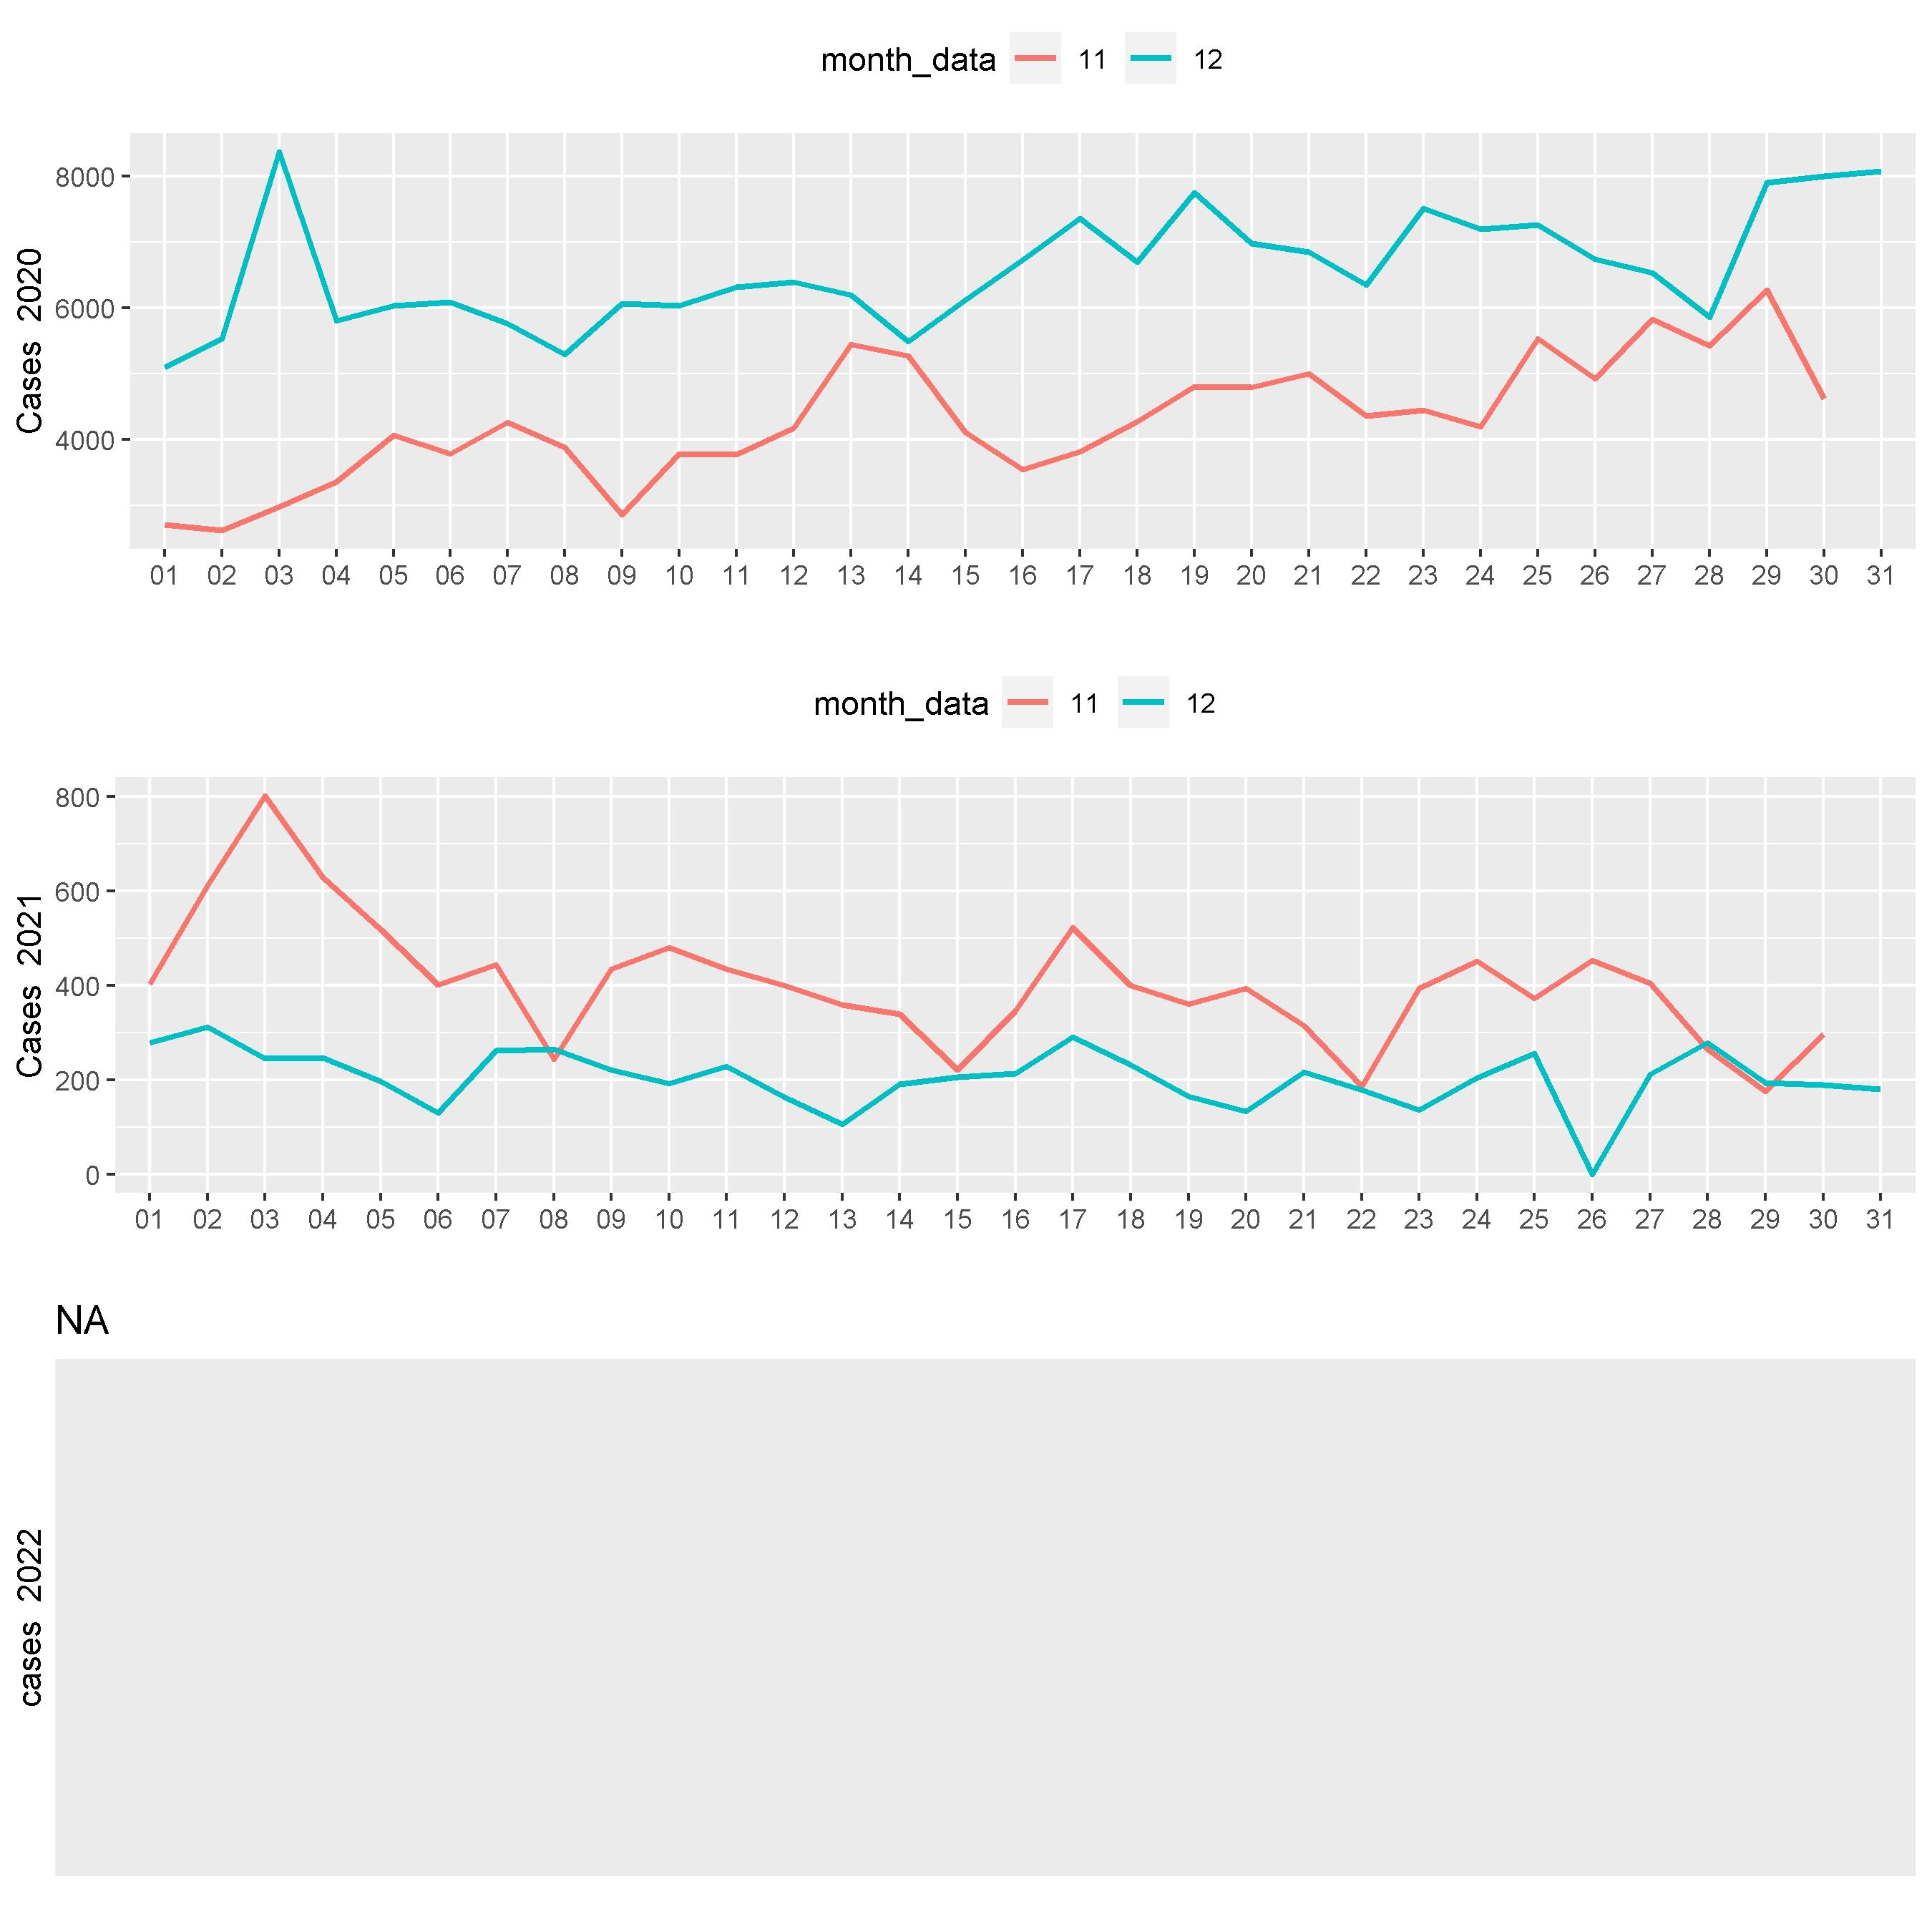
\includegraphics[scale = 0.7]{Images/V/v4 Indonesia .jpeg}
		    \caption{Biểu đồ thể hiện thu thập dữ liệu nhiễm bệnh theo 2 tháng cuối của Indonesia}
		    \label{fig:my_label}
		\end{figure}
		\begin{figure}[htp]
		    \centering
		    \includegraphics[scale = 0.7]{Images/V/v4 Japan .jpeg}
		    \caption{Biểu đồ thể hiện thu thập dữ liệu nhiễm bệnh theo 2 tháng cuối của Nhật Bản}
		    \label{fig:my_label}
		\end{figure}
		\begin{figure}[htp]
		    \centering
		    \includegraphics[scale = 0.7]{Images/V/v4 Vietnam .jpeg}
		    \caption{Biểu đồ thể hiện thu thập dữ liệu nhiễm bệnh theo 2 tháng cuối của Việt Nam}
		    \label{fig:my_label}
		\end{figure}
        \newpage
    %%%%%%%v5%%%%%%
    \newpage
    \item Biểu đồ thể hiện thu thập dữ liệu tử vong gồm 2 tháng cuối của năm
    \begin{lstlisting}[frame=single]  
#v5
country_chart("Vietnam","line_chart","11_12","deaths","v5")
country_chart("Japan","line_chart","11_12","deaths","v5")
country_chart("Indonesia","line_chart","11_12","deaths","v5")
		\end{lstlisting}
        \begin{figure}[htp]
		    \centering
		    \includegraphics[scale = 0.7]{Images/V/v5 Indonesia .jpeg}
		    \caption{Biểu đồ thể hiện thu thập dữ liệu tử vong theo 2 tháng cuối của Indonesia}
		    \label{fig:my_label}
		\end{figure}
		\begin{figure}[htp]
		    \centering
		    \includegraphics[scale = 0.7]{Images/V/v5 Japan .jpeg}
		    \caption{Biểu đồ thể hiện thu thập dữ liệu tử vong theo 2 tháng cuối của Nhật Bản}
		    \label{fig:my_label}
		\end{figure}
		\begin{figure}[htp]
		    \centering
		    \includegraphics[scale = 0.7]{Images/V/v5 Vietnam .jpeg}
		    \caption{Biểu đồ thể hiện thu thập dữ liệu tử vong theo 2 tháng cuối của Việt Nam}
		    \label{fig:my_label}
		\end{figure}
    %%%%%%%v6%%%%%%%%
    \newpage
    \item Biểu đồ thể hiện thu thập dữ liệu gồm nhiễm bệnh và tử vong gồm 2 tháng cuối của năm
    \begin{lstlisting}[frame=single]  
#v6
country_chart("Vietnam","two_line","11_12","","v6")
country_chart("Japan","two_line","11_12","","v6")
country_chart("Indonesia","two_line","11_12","","v6")
		\end{lstlisting}
		\begin{figure}[htp]
		    \centering
		    \includegraphics[scale = 0.7]{Images/V/v6 Indonesia .jpeg}
		    \caption{Biểu đồ thể hiện thu thập dữ liệu nhiễm bệnh và tử vong theo 2 tháng cuối của Indonesia}
		    \label{fig:my_label}
		\end{figure}
		\begin{figure}[htp]
		    \centering
		    \includegraphics[scale = 0.7]{Images/V/v6 Japan .jpeg}
		    \caption{Biểu đồ thể hiện thu thập dữ liệu nhiễm bệnh và tử vong theo 2 tháng cuối của Nhật Bản}
		    \label{fig:my_label}
		\end{figure}
		\begin{figure}[htp]
		    \centering
		    \includegraphics[scale = 0.7]{Images/V/v6 Vietnam .jpeg}
		    \caption{Biểu đồ thể hiện thu thập dữ liệu nhiễm bệnh và tử vong theo 2 tháng cuối của Việt Nam}
		    \label{fig:my_label}
		\end{figure}
    %%%%%%v7%%%%%%%%
    \newpage
    \item Biểu đồ thể hiện thu thập dữ liệu nhiễm bệnh tích lũy cho từng tháng
    \begin{lstlisting}[frame=single]  
#v7
country_chart("Vietnam","cum","2_1_7_9","cases","v7")
country_chart("Japan","cum","2_1_7_9","cases","v7")
country_chart("Indonesia","cum","2_1_7_9","cases","v7")
		\end{lstlisting}
		\begin{figure}[htp]
		    \centering
		    \includegraphics[scale = 0.7]{Images/V/v7 Indonesia .jpeg}
		    \caption{Biểu đồ thể hiện thu thập dữ liệu nhiễm bệnh tích lũy Indonesia}
		    \label{fig:my_label}
		\end{figure}
		\begin{figure}[htp]
		    \centering
		    \includegraphics[scale = 0.7]{Images/V/v7 Japan .jpeg}
		    \caption{Biểu đồ thể hiện thu thập dữ liệu nhiễm bệnh tích lũy của Nhật Bản}
		    \label{fig:my_label}
		\end{figure}
		\begin{figure}[htp]
		    \centering
		    \includegraphics[scale = 0.7]{Images/V/v7 Vietnam .jpeg}
		    \caption{Biểu đồ thể hiện thu thập dữ liệu nhiễm bệnh tích lũy Việt Nam}
		    \label{fig:my_label}
		 \end{figure}
    %%%%%v8%%%%%%%%
    \newpage
    \item Biểu đồ thể hiện thu thập dữ liệu tử vong tích lũy cho từng tháng
    \begin{lstlisting}[frame=single]  
#v8
country_chart("Vietnam","cum","2_1_7_9","deaths","v8")
country_chart("Japan","cum","2_1_7_9","deaths","v8")
country_chart("Indonesia","cum","2_1_7_9","deaths","v8")
		\end{lstlisting}
		\begin{figure}[htp]
		    \centering
		    \includegraphics[scale = 0.7]{Images/V/v8 Indonesia .jpeg}
		    \caption{Biểu đồ thể hiện thu thập dữ liệu tử vong tích lũy Indonesia}
		    \label{fig:my_label}
		\end{figure}
		\begin{figure}[htp]
		    \centering
		    \includegraphics[scale = 0.7]{Images/V/v8 Japan .jpeg}
		    \caption{Biểu đồ thể hiện thu thập dữ liệu tử vong tích lũy của Nhật Bản}
		    \label{fig:my_label}
		\end{figure}
		\begin{figure}[htp]
		    \centering
		    \includegraphics[scale = 0.7]{Images/V/v8 Vietnam .jpeg}
		    \caption{Biểu đồ thể hiện thu thập dữ liệu tử vong tích lũy Việt Nam}
		    \label{fig:my_label}
		 \end{figure}
		 \newpage
\end{enumerate}

%%%%%%%%%%vi%%%%%%%%%
\item \textcolor{red}{Nhóm câu hỏi liên quan đến trực quan dữ liệu theo trung bình 7 ngày gần nhất:}\\
- Với mỗi quốc gia mà thuộc về nhóm, trên từng năm hãy vẽ biểu đồ thể hiện trục Ox là thời gian, trục Oy là nhiễm bệnh/tử vong. Hãy dùng 4 ký số của mã đề để vẽ 4 tháng tương ứng theo ký số đó. Nếu ký số là 0 thì lấy tháng là 10.

- Dùng trung bình của các ca nhiễm bệnh và tử vong được báo cáo trong 7 ngày gần nhất để loại trừ một số báo cáo không thường xuyên và đưa chúng ta đến gần hơn với con số hàng ngày.

\begin{enumerate}[1)]
%%%%%%%vi1%%%%%%%%
    \item Biểu đồ thể hiện thu thập dữ liệu nhiễm bệnh cho từng tháng
    \begin{lstlisting}[frame=single]  
#vi1
country_chart("Vietnam","line_chart","2_1_7_9","cases","vi1","avg")
country_chart("Japan","line_chart","2_1_7_9","cases","vi1","avg")
country_chart("Indonesia","line_chart","2_1_7_9","cases","vi1","avg")
		\end{lstlisting}	
		\begin{figure}[htp]
		    \centering
		    \includegraphics[scale = 0.7]{Images/VI/vi1 Indonesia .jpeg}
		    \caption{Biểu đồ thể hiện thu thập dữ liệu nhiễm bệnh của Indonesia}
		    \label{fig:my_label}
		\end{figure}
		\begin{figure}[htp]
		    \centering
		    \includegraphics[scale = 0.7]{Images/VI/vi1 Japan .jpeg}
		    \caption{Biểu đồ thể hiện thu thập dữ liệu nhiễm bệnh của Nhật Bản}
		    \label{fig:my_label}
		\end{figure}
		\begin{figure}[htp]
		    \centering
		    \includegraphics[scale = 0.7]{Images/VI/vi1 Vietnam .jpeg} 
		    \caption{Biểu đồ thể hiện thu thập dữ liệu nhiễm bệnh của Việt Nam}
		    \label{fig:my_label}
		 \end{figure}
		 \newpage

%%%%%%%vi2%%%%%%%%
    \item Biểu đồ thể hiện thu thập dữ liệu tử vong cho từng tháng
    \begin{lstlisting}[frame=single]  
#vi2
country_chart("Vietnam","line_chart","2_1_7_9","deaths","vi2","avg")
country_chart("Japan","line_chart","2_1_7_9","deaths","vi2","avg")
country_chart("Indonesia","line_chart","2_1_7_9","deaths","vi2","avg")
		\end{lstlisting}
		\begin{figure}[htp]
		    \centering
		    \includegraphics[scale = 0.7]{Images/VI/vi2 Indonesia .jpeg}
		    \caption{Biểu đồ thể hiện thu thập dữ liệu tử vong của Indonesia}
		    \label{fig:my_label}
		\end{figure}
		\begin{figure}[htp]
		    \centering
		    \includegraphics[scale = 0.7]{Images/VI/vi2 Japan .jpeg}
		    \caption{Biểu đồ thể hiện thu thập dữ liệu tử vong của Nhật Bản}
		    \label{fig:my_label}
		\end{figure}
		\begin{figure}[htp]
		    \centering
		    \includegraphics[scale = 0.7]{Images/VI/vi2 Vietnam .jpeg} 
		    \caption{Biểu đồ thể hiện thu thập dữ liệu tử vong của Việt Nam}
		    \label{fig:my_label}
		 \end{figure}
		 \newpage
		%%%%%%%vi3%%%%%%%%
    \item Biểu đồ thể hiện thu thập dữ liệu gồm nhiễm bệnh và tử vong cho từng tháng
    \begin{lstlisting}[frame=single]  
#vi3
country_chart("Vietnam","two_line","2_1_7_9","","vi3","avg")
country_chart("Japan","two_line","2_1_7_9","","vi3","avg")
country_chart("Indonesia","two_line","2_1_7_9","","vi3","avg")
		\end{lstlisting}	
		\begin{figure}[htp]
		    \centering
		    \includegraphics[scale = 0.7]{Images/VI/vi3 Indonesia .jpeg}
		    \caption{Biểu đồ thể hiện thu thập dữ liệu nhiễm bệnh và tử vong của Indonesia}
		    \label{fig:my_label}
		\end{figure}
		\begin{figure}[htp]
		    \centering
		    \includegraphics[scale = 0.7]{Images/VI/vi3 Japan .jpeg}
		    \caption{Biểu đồ thể hiện thu thập dữ liệu nhiễm bệnh và tử vong của Nhật Bản}
		    \label{fig:my_label}
		\end{figure}
		\begin{figure}[htp]
		    \centering
		    \includegraphics[scale = 0.7]{Images/VI/vi3 Vietnam .jpeg} 
		    \caption{Biểu đồ thể hiện thu thập dữ liệu nhiểm bệnh và tử vong của Việt Nam}
		    \label{fig:my_label}
		 \end{figure}
		 \newpage
		%%%%%%%vi4%%%%%%%%
    \item Biểu đồ thể hiện thu thập dữ liệu nhiễm bệnh gồm 2 tháng cuối của năm
    \begin{lstlisting}[frame=single]  
#vi4
country_chart("Vietnam","line_chart","11_12","cases","vi4","avg")
country_chart("Japan","line_chart","11_12","cases","vi4","avg")
country_chart("Indonesia","line_chart","11_12","cases","vi4","avg")
		\end{lstlisting}
		\begin{figure}[htp]
		    \centering
		    \includegraphics[scale = 0.7]{Images/VI/vi4 Indonesia .jpeg}
		    \caption{Biểu đồ thể hiện thu thập dữ liệu nhiễm bệnh theo 2 tháng cuối năm của Indonesia}
		    \label{fig:my_label}
		\end{figure}
		\begin{figure}[htp]
		    \centering
		    \includegraphics[scale = 0.7]{Images/VI/vi4 Japan .jpeg}
		    \caption{Biểu đồ thể hiện thu thập dữ liệu nhiễm bệnh theo 2 tháng cuối năm của Nhật Bản}
		    \label{fig:my_label}
		\end{figure}
		\begin{figure}[htp]
		    \centering
		    \includegraphics[scale = 0.7]{Images/VI/vi4 Vietnam .jpeg} 
		    \caption{Biểu đồ thể hiện thu thập dữ liệu nhiểm bệnh theo 2 tháng cuối năm của Việt Nam}
		    \label{fig:my_label}
		 \end{figure}
		 \newpage
		%%%%%%%vi5%%%%%%%%
    \item Biểu đồ thể hiện thu thập dữ liệu tử vong gồm 2 tháng cuối của năm
    \begin{lstlisting}[frame=single]  
#vi5
country_chart("Vietnam","line_chart","11_12","deaths","vi5","avg")
country_chart("Japan","line_chart","11_12","deaths","vi5","avg")
country_chart("Indonesia","line_chart","11_12","deaths","vi5","avg")
		\end{lstlisting}
		\begin{figure}[htp]
		    \centering
		    \includegraphics[scale = 0.7]{Images/VI/vi5 Indonesia .jpeg}
		    \caption{Biểu đồ thể hiện thu thập dữ liệu tử vong theo 2 tháng cuối năm của Indonesia}
		    \label{fig:my_label}
		\end{figure}
		\begin{figure}[htp]
		    \centering
		    \includegraphics[scale = 0.7]{Images/VI/vi5 Japan .jpeg}
		    \caption{Biểu đồ thể hiện thu thập dữ liệu tử vong theo 2 tháng cuối năm của Nhật Bản}
		    \label{fig:my_label}
		\end{figure}
		\begin{figure}[htp]
		    \centering
		    \includegraphics[scale = 0.7]{Images/VI/vi5 Vietnam .jpeg} 
		    \caption{Biểu đồ thể hiện thu thập dữ liệu tử vong theo 2 tháng cuối năm của Việt Nam}
		    \label{fig:my_label}
		 \end{figure}
		 \newpage
		%%%%%%%vi6%%%%%%%%
    \item Biểu đồ thể hiện thu thập dữ liệu gồm nhiễm bệnh và tử vong gồm 2 tháng cuối của năm
   \begin{lstlisting}[frame=single]  
#vi6
country_chart("Vietnam","two_line","11_12","","vi6","avg")
country_chart("Japan","two_line","11_12","","vi6","avg")
country_chart("Indonesia","two_line","11_12","","vi6","avg")
		\end{lstlisting}	
		\begin{figure}[htp]
		    \centering
		    \includegraphics[scale = 0.7]{Images/VI/vi6 Indonesia .jpeg}
		    \caption{Biểu đồ thể hiện thu thập dữ liệu nhiễm bệnh và tử vong theo 2 tháng cuối năm của Indonesia}
		    \label{fig:my_label}
		\end{figure}
		\begin{figure}[htp]
		    \centering
		    \includegraphics[scale = 0.7]{Images/VI/vi6 Japan .jpeg}
		    \caption{Biểu đồ thể hiện thu thập dữ liệu nhiễm bệnh và tử vong theo 2 tháng cuối năm của Nhật Bản}
		    \label{fig:my_label}
		\end{figure}
		\begin{figure}[htp]
		    \centering
		    \includegraphics[scale = 0.7]{Images/VI/vi6 Vietnam .jpeg} 
		    \caption{Biểu đồ thể hiện thu thập dữ liệu nhiễm bệnh và tử vong theo 2 tháng cuối năm của Việt Nam}
		    \label{fig:my_label}
		 \end{figure}
		 \newpage
		%%%%%%%vi7%%%%%%%%
    \item Biểu đồ thể hiện thu thập dữ liệu nhiễm bệnh tích lũy cho từng tháng
    \begin{lstlisting}[frame=single]  
#vi7
country_chart("Vietnam","cum","2_1_7_9","cases","vi7","avg")
country_chart("Japan","cum","2_1_7_9","cases","vi7","avg")
country_chart("Indonesia","cum","2_1_7_9","cases","vi7","avg")
		\end{lstlisting}
		\begin{figure}[htp]
		    \centering
		    \includegraphics[scale = 0.7]{Images/VI/vi7 Indonesia .jpeg}
		    \caption{Biểu đồ thể hiện thu thập dữ liệu nhiễm bệnh tích lũy cho từng tháng của Indonesia}
		    \label{fig:my_label}
		\end{figure}
		\begin{figure}[htp]
		    \centering
		    \includegraphics[scale = 0.7]{Images/VI/vi7 Japan .jpeg}
		    \caption{Biểu đồ thể hiện thu thập dữ liệu nhiễm bệnh tích lũy cho từng tháng của Nhật Bản}
		    \label{fig:my_label}
		\end{figure}
		\begin{figure}[htp]
		    \centering
		    \includegraphics[scale = 0.7]{Images/VI/vi7 Vietnam .jpeg} 
		    \caption{Biểu đồ thể hiện thu thập dữ liệu nhiễm bệnh tích lũy cho từng tháng của Việt Nam}
		    \label{fig:my_label}
		 \end{figure}
		 \newpage
    
    %%%%%%%vi8%%%%%%%%
    \item Biểu đồ thể hiện thu thập dữ liệu tử vong tích lũy cho từng tháng
\begin{lstlisting}[frame=single]  
#vi8
country_chart("Vietnam","cum","2_1_7_9","deaths","vi8","avg")
country_chart("Japan","cum","2_1_7_9","deaths","vi8","avg")
country_chart("Indonesia","cum","2_1_7_9","deaths","vi8","avg")
		\end{lstlisting}	
		\begin{figure}[htp]
		    \centering
		    \includegraphics[scale = 0.7]{Images/VI/vi8 Indonesia .jpeg}
		    \caption{Biểu đồ thể hiện thu thập dữ liệu tử vong tích lũy cho từng tháng của Indonesia}
		    \label{fig:my_label}
		\end{figure}
		\begin{figure}[htp]
		    \centering
		    \includegraphics[scale = 0.7]{Images/VI/vi8 Japan .jpeg}
		    \caption{Biểu đồ thể hiện thu thập dữ liệu tử vong tích lũy cho từng tháng của Nhật Bản}
		    \label{fig:my_label}
		\end{figure}
		\begin{figure}[htp]
		    \centering
		    \includegraphics[scale = 0.7]{Images/VI/vi8 Vietnam .jpeg} 
		    \caption{Biểu đồ thể hiện thu thập dữ liệu tử vong tích lũy cho từng tháng của Việt Nam}
		    \label{fig:my_label}
		 \end{figure}
		 \newpage
\end{enumerate}

\item \textcolor{red}{Nhóm câu hỏi liên quan đến tất cả quốc gia theo thời gian là tháng }

- Trên từng năm hãy vẽ biểu đồ thể hiện trục Ox là thời gian, trục Oy là nhiễm bệnh/tử vong. Hãy dùng 4 ký số của mã đề để vẽ 4 tháng tương ứng theo ký số đó. Nếu ký số là 0 thì lấy tháng là 10. 
\begin{enumerate}[1)]

    %%%%%%%vii1%%%%%%%%
    \item Biểu đồ thể hiện thu thập dữ liệu nhiễm bệnh theo thời gian là tháng của tất cả quốc gia
\begin{lstlisting}[frame=single]  
#vii1
country_chart("World","line_chart","2_1_7_9","cases","vii1")
		\end{lstlisting}	
        \begin{figure}[htp]
		    \centering
		    \includegraphics[scale = 0.7]{Images/VII/vii1 World .jpeg} 
		    \caption{Biểu đồ thể hiện thu thập dữ liệu nhiễm bệnh theo thời gian là tháng của tất cả quốc gia}
		    \label{fig:my_label}
		\end{figure}
		\newpage
    %%%%%%%vii2%%%%%%%%
    \item Biểu đồ thể hiện thu thập dữ liệu tử vong theo thời gian là tháng của tất cả quốc gia
    \begin{lstlisting}[frame=single]  
#vii2
country_chart("World","line_chart","2_1_7_9","deaths","vii2")
		\end{lstlisting}
    \begin{figure}[htp]
		    \centering
		    \includegraphics[scale = 0.7]{Images/VII/vii2 World .jpeg}
		    \caption{Biểu đồ thể hiện thu thập dữ liệu tử vong theo thời gian là tháng của tất cả quốc gia}
		    \label{fig:my_label}
		\end{figure}
		\newpage
    %%%%%%%vii3%%%%%%%%
    \item Biểu đồ thể hiện thu thập dữ liệu nhiễm bệnh theo thời gian là 2 tháng cuối của năm của tất cả quốc giaị
    \begin{lstlisting}[frame=single]  
#vii3
country_chart("World","line_chart","11_12","cases","vii3")
		\end{lstlisting}
    \begin{figure}[htp]
		    \centering
		    \includegraphics[scale = 0.7]{Images/VII/vii3 World .jpeg}
		    \caption{Biểu đồ thể hiện thu thập dữ liệu nhiễm bệnh theo thời gian là 2 tháng cuối của tất cả quốc gia}
		    \label{fig:my_label}
		\end{figure}
		\newpage
    %%%%%%%vii4%%%%%%%%
    \item Biểu đồ thể hiện thu thập dữ liệu tử vong theo thời gian là 2 tháng cuối của năm của tất cả quốc gia
    \begin{lstlisting}[frame=single]  
#vii4
country_chart("World","line_chart","11_12","deaths","vii4")
		\end{lstlisting}
		\begin{figure}[htp]
		    \centering
		    \includegraphics[scale = 0.7]{Images/VII/vii4 World .jpeg}
		    \caption{Biểu đồ thể hiện thu thập dữ liệu tử vong theo thời gian là 2 tháng cuối của năm của tất cả quốc gia}
		    \label{fig:my_label}
		\end{figure}
		\newpage
    %%%%%%%vii5%%%%%%%%
    \item Biểu đồ thể hiện thu thập dữ liệu nhiễm bệnh tương đối tích lũy theo thời gian là 2 tháng cuối của năm của tất cả quốc giaị
    \begin{lstlisting}[frame=single]  
#vii5
country_chart("World","cum_rel","11_12","cases","vii5")
		\end{lstlisting}
		\begin{figure}[htp]
		    \centering
		    \includegraphics[scale = 0.7]{Images/VII/vii5 World .jpeg}
		    \caption{Biểu đồ thể hiện thu thập dữ liệu nhiễm bệnh tương đối tích lũy theo thời gian là 2 tháng cuối của năm của tất cả quốc gia}
		    \label{fig:my_label}
		\end{figure}
		\newpage
    %%%%%%%vii6%%%%%%%%
    \item Biểu đồ thể hiện thu thập dữ liệu tử vong tương đối tích lũy theo thời gian là 2 tháng cuối của năm của tất cả quốc gia
    \begin{lstlisting}[frame=single]  
#vii6
country_chart("World","cum_rel","11_12","deaths","vii6")
		\end{lstlisting}
		\begin{figure}[htp]
		    \centering
		    \includegraphics[scale = 0.7]{Images/VII/vii6 World .jpeg}
		    \caption{Biểu đồ thể hiện thu thập dữ liệu tử vong tương đối tích lũy theo thời gian là 2 tháng cuối của năm của tất cả quốc gia}
		    \label{fig:my_label}
		\end{figure}
\end{enumerate}
\item \textcolor{red}{Nhóm câu hỏi liên quan đến tất cả quốc gia theo trung bình 7 ngày gần nhất}\\
Trên từng năm hãy vẽ biểu đồ thể hiện trục Ox là thời gian, trục Oy là nhiễm bệnh/tử vong. Hãy dùng 4 ký số của mã đề để vẽ 4 tháng tương ứng theo ký số đó. Nếu ký số là 0 thì lấy tháng là 10. 
\begin{enumerate}[1)]
    %%%%%%%viii1%%%%%%%%
    \newpage
    \item Biểu đồ thể hiện thu thập dữ liệu nhiễm bệnh theo thời gian là tháng của tất cả quốc gia theo trung bình 7 ngày gần nhất
    \begin{lstlisting}
#viii1
country_chart("World","line_chart","2_1_7_9","cases","viii1","avg")
    \end{lstlisting}
    \begin{figure}[htp]
        \centering
		\includegraphics[scale = 0.7]{Images/VIII/viii1 World .jpeg} 
		\caption{Biểu đồ thể hiện thu thập dữ liệu nhiễm bệnh theo thời gian là tháng của tất cả quốc gia}
		\label{fig:my_label}
	\end{figure}
	\newpage
	
    %%%%%%%viii2%%%%%%%%
    \item Biểu đồ thể hiện thu thập dữ liệu tử vong theo thời gian là tháng của tất cả quốc gia theo trung bình 7 ngày gần nhất
    
    \begin{lstlisting}
#viii2
country_chart("World","line_chart","2_1_7_9","deaths","viii2","avg")
    \end{lstlisting}
    \begin{figure}[htp]
        \centering
		\includegraphics[scale = 0.7]{Images/VIII/viii2 World .jpeg} 
		\caption{Biểu đồ thể hiện thu thập dữ liệu tử vong theo thời gian là tháng của tất cả quốc gia}
		\label{fig:my_label}
	\end{figure}
	\newpage
	
    %%%%%%%viii3%%%%%%%%
    \item Biểu đồ thể hiện thu thập dữ liệu nhiễm bệnh theo thời gian là 2 tháng của năm của tất cả quốc giaị theo trung bình 7 ngày gần nhất
    \begin{lstlisting}
#viii3
country_chart("World","line_chart","11_12","cases","viii3","avg")
    \end{lstlisting}
    \begin{figure}[htp]
        \centering
		\includegraphics[scale = 0.7]{Images/VIII/viii3 World .jpeg} 
		\caption{Biểu đồ thể hiện thu thập dữ liệu nhiễm bệnh theo thời gian là 2 tháng của năm của tất cả quốc giaị theo trung bình 7 ngày gần nhất}
		\label{fig:my_label}
	\end{figure}
	\newpage
	
    %%%%%%%viii4%%%%%%%%
    \item Biểu đồ thể hiện thu thập dữ liệu tử vong theo thời gian là 2 tháng của năm của tất cả quốc gia theo trung bình 7 ngày gần nhất
    \begin{lstlisting}
#viii4
country_chart("World","line_chart","11_12","deaths","viii4","avg")   
    \end{lstlisting}
    \begin{figure}[htp]
        \centering
		\includegraphics[scale = 0.7]{Images/VIII/viii4 World .jpeg} 
		\caption{Biểu đồ thể hiện thu thập dữ liệu tử vong theo thời gian là 2 tháng của năm của tất cả quốc gia theo trung bình 7 ngày gần nhất}
		\label{fig:my_label}
	\end{figure}
	\newpage
	
    %%%%%%%viii5%%%%%%%%
    \item Biểu đồ thể hiện thu thập dữ liệu nhiễm bệnh tích lũy theo thời gian là 2 tháng của năm của tất cả quốc giaị theo trung bình 7 ngày gần nhất
    \begin{lstlisting}
#viii5
country_chart("World","cum","11_12","cases","viii5","avg")    
    \end{lstlisting}
    \begin{figure}[htp]
        \centering
		\includegraphics[scale = 0.7]{Images/VIII/viii5 World .jpeg} 
		\caption{Biểu đồ thể hiện thu thập dữ liệu nhiễm bệnh tích lũy theo thời gian là 2 tháng của năm của tất cả quốc giaị theo trung bình 7 ngày gần nhất}
		\label{fig:my_label}
	\end{figure}
	\newpage
	
    %%%%%%%viii6%%%%%%%%
    \item Biểu đồ thể hiện thu thập dữ liệu tử vong tích lũy theo thời gian là 2 tháng của năm của tất cả quốc gia theo trung bình 7 ngày gần nhất
    \begin{lstlisting}
#viii6
country_chart("World","cum","11_12","deaths","viii6","avg")      
    \end{lstlisting}
    \begin{figure}[htp]
        \centering
		\includegraphics[scale = 0.7]{Images/VIII/viii6 World .jpeg} 
		\caption{Biểu đồ thể hiện thu thập dữ liệu tử vong tích lũy theo thời gian là 2 tháng của năm của tất cả quốc gia theo trung bình 7 ngày gần nhất}
		\label{fig:my_label}
	\end{figure}
	\newpage
\end{enumerate}

%%%%%%ix)%%%%%%%%
\item \textcolor{red}{Nhóm câu hỏi liên quan đến sự tương quan giữa nhiễm bệnh và tử vong}
    \begin{enumerate}[1)]
    %%%%%%ix1)%%%%%%%%
        \item Vẽ biểu đồ thể hiện phần trăm giữa nhiễm bệnh tích lũy trên tổng nhiễm bệnh và phần trăm tử vong tích lũy trên tổng số tử vong cho từng quốc gia theo thời gian. Vẽ 2 đường trên cùng biểu đồ\\
        
        Trên từng quốc gia riêng của nhóm hãy vẽ biểu đồ thể hiện trục Ox là nhiễm bệnh, trục Oy là tử vong. Hãy lấy 4 tháng theo 4 ký số mã đề thể hiện. Nếu ký số là 0 thì lấy tháng là 10.
        
        \begin{lstlisting}[frame=single]
#pre ix1
  need_con <- c("Vietnam", "Japan", "Indonesia")
  #need_month <- c("02", "01", "07", "09")
  three_country <- data %>% filter(location %in% need_con)
  three_country$date <- as.POSIXct(three_country$date, 
                                format = "%m/ %d/ %Y")
  
  row.names(three_country) <- 1:nrow(three_country)
  
  Vie<-three_country%>%filter(three_country$location== "Vietnam")
  Jap<-three_country%>%filter(three_country$location== "Japan")
  In<-three_country%>%filter(three_country$location== "Indonesia")
  options("scipen"=10)
  #View(Vie)
  #function
  draw_chart <- function(country_data, country_name)
  {
    new_cases_data <- country_data$new_cases
    new_deaths_data <- country_data$new_deaths
    sum_cases <- sum(new_cases_data, na.rm = TRUE)
    sum_deaths <- sum(new_deaths_data, na.rm = TRUE)
    cases_cumu <- cbind(new_cases_data)
    deaths_cumu <- cbind(new_deaths_data)
    cases_cumu[is.na(cases_cumu)] <- 0
    deaths_cumu[is.na(deaths_cumu)] <- 0
    for(x in 1:(length(new_cases_data) - 1))
    {
      cases_cumu[x + 1] <- cases_cumu[x] + cases_cumu[x + 1]
      deaths_cumu[x + 1] <- deaths_cumu[x] + deaths_cumu[x + 1]
    }
    for(x in 1:length(new_cases_data))
    {
      cases_cumu[x] <- (cases_cumu[x] / sum_cases)*100
      deaths_cumu[x] <- (deaths_cumu[x] / sum_deaths)*100
    }
    name = country_data
    name = name$date
    chart_data <- data.frame(name, cases_cumu, deaths_cumu)
    #View(chart_data)
    title = paste(country_name, " New_cases and New_deaths line chart")
    line_chart <- ggplot(data = chart_data, aes(x = name))+
      geom_line(aes(y=cases_cumu,colour="New_cases"),size=1.2)+
      geom_line(aes(y=deaths_cumu,colour="New_deaths"),size=1.2)+
      ylab("New_cases and New_deaths percent")+
      xlab("Month")+
      ylab("Percent")+
      theme(text = element_text(size = 16))+
      ggtitle(title)
    return(line_chart)
  }
  
  #ix1
  ix1 <- function()
  {
    #View(Vie)
    Vie_chart <- draw_chart(Vie[,3:6], "Vietnam")
    ggsave(filename = "ix1Vietnam.jpeg", plot = Vie_chart, 
    device = "jpeg", scale = 1, width = 8, height = 8)
    Jap_chart <- draw_chart(Jap[,3:6], "Japan")
    ggsave(filename = "ix1Japan.jpeg", plot = Jap_chart, 
    device = "jpeg", scale = 1, width = 8, height = 8)
    In_chart <- draw_chart(In[,3:6], "Indonesia")
    ggsave(filename = "ix1Indonesia.jpeg", plot = In_chart, 
    device = "jpeg", scale = 1, width = 8, height = 8)
  }
ix1()
        \end{lstlisting}
        \begin{itemize}
            \item Biến three\_country nhận vào dữ liệu của 3 nước Indonesia, Nhật Bản, Việt Nam. Sử dụng $as.POSIXct$ để định dạng lại ngày tháng năm và chuyển kiểu dữ liệu của cột date thành kiểu dữ liệu $Date$.\\
            \item Tách dữ liệu ra theo từng nước và gán vào các biến In(Indonesia),
            Jap(Nhật Bản), Vie(Việt Nam) để hỗ trợ cho việc vẽ biểu đồ theo từng nước.\\
            \item Hàm $draw\_chart$ sẽ trả về biểu đồ cần vẽ theo quốc gia, hàm chứa các tham số:\\
                \begin{itemize}
                    \item $country\_data$: Tham số chứa dữ liệu của quốc gia cần vẽ biểu đồ.\\
                    \item $country\_name$: Tham số chứ tên của quốc gia cần vẽ vẽ biểu đồ.\\
                \end{itemize}
            \item Hàm $ggsave()$ dùng để xuất biểu đồ theo định dạng ảnh.\\
        \end{itemize}
        \newpage
        \begin{figure}[h!]
            \centering
            \includegraphics[scale = 0.8]{Images/IX/ix1Indonesia.jpeg}
            \label{fig:my_label}
        \end{figure}
        \begin{figure}[h!]
            \begin{center}
            \caption{Biểu đồ thể hiện phần trăm giữa nhiễm bệnh tích lũy trên tổng nhiễm bệnh và phần trăm tử vong tích lũy trên tổng số tử vong của Indonesia}
	        \end{center}
        \end{figure}
        \newpage
        \begin{figure}[h!]
            \centering
            \includegraphics[scale = 0.8]{Images/IX/ix1Japan.jpeg}
            \label{fig:my_label}
        \end{figure}
        \begin{figure}[h!]
            \begin{center}
            \caption{Biểu đồ thể hiện phần trăm giữa nhiễm bệnh tích lũy trên tổng nhiễm bệnh và phần trăm tử vong tích lũy trên tổng số tử vong của Nhật Bản}
	        \end{center}
        \end{figure}
        \newpage
        \begin{figure}[h!]
            \centering
            \includegraphics[scale = 0.8]{Images/IX/ix1Vietnam.jpeg}
            \label{fig:my_label}
        \end{figure}
        \begin{figure}[h!]
            \begin{center}
            \caption{Biểu đồ thể hiện phần trăm giữa nhiễm bệnh tích lũy trên tổng nhiễm bệnh và phần trăm tử vong tích lũy trên tổng số tử vong của Việt Nam}
	        \end{center}
        \end{figure}
\newpage
      %%%%%%func and prep%%%%%%%%  
        \lstset{
    title=Function and Prep for ix 2-3}
\begin{lstlisting}[frame=single]  
ix_cor_MY <- function(subdata, stt_month)
{
  data_my <- subdata %>% mutate(date = mdy(date),
                Month_Yr = format_ISO8601(date, precision = "ym"))
  data_my <- subset(data_my, !is.na(data_my[,5]))
  data_my <- subset(data_my, !is.na(data_my[,6]))
  subMonth <- subset(data_my, Month_Yr == stt_month)
  if(nrow(subMonth) == 0)
  {
    plot(NULL, xlim=c(0,1), ylim=c(0,1), main = stt_month, 
        sub = paste("No Correlation"), ylab="Deaths", xlab="Cases")
    abline(h = 0.5, col = "red", lwd = 3)
  }
  else
  {
    if(nrow(subMonth) == 1)
    {
      plot(subMonth[,5], subMonth[,6], pch = 10, col = "black", 
            main = stt_month, sub = paste("No Correlation"), 
            ylab="Deaths", xlab="Cases")
      abline(h = subMonth[1,6], col = "red", lwd = 3)
    }
    else 
    {
      num <- cor(subMonth[,5], subMonth[,6], method = "pearson")
      if(is.na(num)) plot(subMonth[,5], subMonth[,6], pch = 10, 
                            col = "black", main = stt_month, 
                            sub = paste("No Correlation"), 
                            ylab="Deaths", xlab="Cases")
      else plot(subMonth[,5], subMonth[,6], pch = 10, col = "black", 
                main = stt_month, 
                sub = paste("Correlation: ", round(num,2)), 
                ylab="Deaths", xlab="Cases")
      abline(lm(subMonth[,6] ~ subMonth[,5]), col = "red", lwd = 3)
    }
  }
}

id_data <- subset(data, location == "Indonesia")
jp_data <- subset(data, location == "Japan")
vn_data <- subset(data, location == "Vietnam")
my_months <- c("2020-01", "2020-02", "2020-07", "2020-09", "2021-01",
                "2021-02", "2021-07", "2021-09", "2022-01", "2022-02")
\end{lstlisting}
\begin{itemize}
    \item Hàm $ix\_cor\_MY$ có tác dụng nhận vào data frame của một đất nước với biến truyền là $subdata$ và tên của một tháng được viết theo định dạng $"YYYY-MM"$ vào biến $stt\_month$ và vẽ ra biểu đồ tương quan dựa trên dữ liệu trong tháng đó của quốc gia mong muốn.
    \item Hàm này sẽ xét cột $date$ của $subdata$ vừa nhập vào và tiến hành tạo ra một cột mới chỉ chứa tháng và năm dựa trên ngày tương ứng của cột $date$ và chuyển data frame mới này vào một biến mới là $data\_my$. Sau đó $data\_my$ này sẽ loại tất cả những hàng không phù hợp với 3 tiêu chí sau: dữ liệu cột $new\_case$ không phải $NA$, dữ liệu cột $new\_death$ không phải $NA$, tháng ở cột mới vừa tạo phải khớp với tên của tháng trong biến $stt\_month$. Sau đó là tiếp tục đưa data frame mới này vào biến $subMonth$. Với dữ liệu đã được xử lý xong, ta tiến hành vễ biểu đồ.
    \item Nếu data frame của biến $subMonth$ có số hàng là $0$ thì nghĩa là trong tháng đó không có dữ liệu để có thể xét tương quan được. Vậy ta sẽ vẽ một biểu đồ rỗng với một đường nằm ngang và in ra dòng chữ $"No Correlation"$ dưới biểu đồ.
    \item Nếu data frame của biến $subMonth$ có số hàng là $1$ thì nghĩa là trong tháng đó chỉ có duy nhất 1 dữ liệu và nhiêu đó là không đủ để có thể xét tương quan được.  Vậy ta cũng sẽ vẽ một biểu đồ với chỉ duy nhất một điểm tượng trưng cho dữ liệu duy nhất đó và một đường nằm ngang tại vị trí của điểm đó và in ra dòng chữ $"No Correlation"$ dưới biểu đồ.
    \item Nếu 2 điều trên không xảy ra nghĩa là dữ liệu của ta có thể tính được tương quan. Ta tính hệ số tương quan này bằng cách dùng hàm $cor(cột new\_case, cột\_new death, method = "pearson")$ để tính hệ số tương quan pearson cho 2 cột nhiễm và tử vong của dữ liệu. Ta đưa hệ số tương quan này vào biến $num$.
    \item Nếu biến $num$ có giá trị là $NA$, nghĩa là một hoặc hai cột trong dữ liệu mang các giá trị giống hệt nhau và điều này không thể cho ta thấy được sự tương quan giữa 2 dữ liệu nhiễm và tử vong. Ta tiến hành vẽ một biểu đồ với các điểm dựa trên dữ liệu nhiễm và tử vong theo từng cặp sau đó dùng thêm hàm $lm()$ để vẽ một đường tuyến tính dựa trên xu hướng của các điểm trên biểu đồ. Vì các giá trị không có tương quan nên đường này sẽ là một đường ngang. Ở dưới biểu đồ sẽ in ra dòng chữ $"No Correlation"$.
    \item Nếu biến $num$ không phải $NA$ thì nghĩa là dữ liệu của ta có sự tương quan. Ta cũng tiến hành vẽ biểu đồ như khi $num$ là $NA$ tuy nhiên ở dưới biểu đồ sẽ là hệ số tương quan của dữ liệu mà ta vừa tính được làm tròn lên 2 chữ số thập phân.
    \item Đoạn code ở dưới hàm là các câu lệnh để lấy ra dữ liệu của 3 nước thuộc về nhóm cần tính cũng như tạo ra 1 vector chứa tên các tháng cần tính tương quan. Với điều này, ở mỗi quốc gia ta sẽ chỉ cần chạy 1 vòng lặp $for$ cho từng giá trị tháng trong vector chứa tháng và xài hàm để vẽ biểu đồ tương quan cho dữ liệu của quốc gia đó với tất cả các tháng chứa trong vector. Đồng thời ta sẽ xài câu lệnh $par(mfrow=c(3,4))$ điều chỉnh layout của bảng plot để hiện được cùng lúc nhiều biểu đồ.
\end{itemize}

\newpage
%%%%%%ix2)%%%%%%%%
        \item Xét tương quan trong mỗi tháng
        \lstset{
    title=Source code for Indonesia}
\begin{lstlisting}[frame=single]  
par(mfrow=c(3,4))
for(i in 1:length(my_months))
{
  ix_cor_MY(id_data,my_months[i])
}
\end{lstlisting}
\begin{figure}[h!]
	\begin{center}
	    \includegraphics[scale=0.8]{Images/IV/Indo.png}
        \label{fig:my_label}
	\end{center}
\end{figure}.
\begin{figure}[h!]
    \begin{center}
	    \caption{Biểu đồ thể hiện tương quan trên từng tháng của Indonesia}
	\end{center}
\end{figure}

\newpage
\lstset{
    title=Source code for Japan}
\begin{lstlisting}[frame=single]  
par(mfrow=c(3,4))
for(i in 1:length(my_months))
{
  ix_cor_MY(jp_data,my_months[i])
}
\end{lstlisting}
\begin{figure}[h!]
	\begin{center}
	    \includegraphics[scale=0.8]{Images/IV/Japan.png}
        \label{fig:my_label}
	\end{center}
\end{figure}
\begin{figure}[h!]
    \begin{center}
	    \caption{Biểu đồ thể hiện tương quan trên từng tháng của Nhật Bản}
	\end{center}
\end{figure}
\newpage
\lstset{
    title=Source code for Vietnam}
\begin{lstlisting}[frame=single]  
par(mfrow=c(3,4))
for(i in 1:length(my_months))
{
  ix_cor_MY(vn_data,my_months[i])
}
\end{lstlisting}
\begin{figure}[h!]
	\begin{center}
	    \includegraphics[scale=0.8]{Images/IV/Vietnam.png}
        \label{fig:my_label}
	\end{center}
\end{figure}
\begin{figure}[h!]
    \begin{center}
	    \caption{Biểu đồ thể hiện tương quan trên từng tháng của Việt Nam}
	\end{center}
\end{figure}
\newpage

%%%%%%ix3)%%%%%%%%
        \item Xét tương quan trong mỗi tháng theo trung bình 7 ngày gần nhất
        \lstset{
    title=Avg 7 days function and Prep for ix3}
\begin{lstlisting}[frame=single]  
avg7 <- function(subdata,col)
{
  new_avg7 <- subdata[,col]
  j <- 1
  for(i in 1:length(new_avg7))
  {
    new_avg7[i] <- (sum(new_avg7[j:i],na.rm = TRUE)/(i-j+1))
    if(i >= 7) j <- j + 1
  }
  return(new_avg7)
}

id_data[,5] <- avg7(id_data,5)
id_data[,6] <- avg7(id_data,6)
jp_data[,5] <- avg7(jp_data,5)
jp_data[,6] <- avg7(jp_data,6)
vn_data[,5] <- avg7(vn_data,5)
vn_data[,6] <- avg7(vn_data,6)
\end{lstlisting}
\begin{itemize}
    \item Hàm $avg7$ có tác dụng nhận vào dữ liệu của một quốc gia và cột cần tính và trả về một cột mới đã được điều chỉnh giá trị theo công thức tính trung bình 7 ngày dựa trên dữ liệu tại cột cần tính của quốc gia nhập vào.
    \item Ta sẽ dùng hàm này để biến đổi các cột nhiễm và tử vong của 3 quốc gia thuộc về nhóm cần tính bằng giá trị đã được chỉnh sửa theo công thức tính trung bình 7 ngày.
    \item Sau khi đã có dữ liệu mới, ta chỉ việc áp dụng cách làm cũ của câu $ix-2$ để vẽ các biểu đồ tương quan mới dựa trên dữ liệu trung bình 7 ngày.
\end{itemize}

        \lstset{
    title=Source code for Indonesia}
    \newpage
\begin{lstlisting}[frame=single]  
par(mfrow=c(3,4))
for(i in 1:length(my_months))
{
  ix_cor_MY(id_data,my_months[i])
}
\end{lstlisting}
\begin{figure}[h!]
	\begin{center}
	    \includegraphics[scale=0.8]{Images/IV/Indo (avg7).png}
        \label{fig:my_label}
	\end{center}
\end{figure}
\begin{figure}[h!]
    \begin{center}
	    \caption{Biểu đồ thể hiện tương quan trên từng tháng của Indonesia theo trung bình 7 ngày gần nhất}
	\end{center}
\end{figure}
\newpage
\lstset{
    title=Source code for Japan}
\begin{lstlisting}[frame=single]  
par(mfrow=c(3,4))
for(i in 1:length(my_months))
{
  ix_cor_MY(jp_data,my_months[i])
}
\end{lstlisting}
\begin{figure}[h!]
	\begin{center}
	    \includegraphics[scale=0.8]{Images/IV/Japan (avg7).png}
	    \label{fig:my_label}
	\end{center}
\end{figure}
\begin{figure}[h!]
    \begin{center}
	    \caption{Biểu đồ thể hiện tương quan trên từng tháng của Nhật Bản theo trung bình 7 ngày gần nhất}
	\end{center}
\end{figure}
\newpage
\lstset{
    title=Source code for Vietnam}
\begin{lstlisting}[frame=single]  
par(mfrow=c(3,4))
for(i in 1:length(my_months))
{
  ix_cor_MY(vn_data,my_months[i])
}
\end{lstlisting}
\begin{figure}[h!]
	\begin{center}
	    \includegraphics[scale=0.8]{Images/IV/Vietnam (avg7).png}
	    \label{fig:my_label}
	\end{center}
\end{figure}
\begin{figure}[h!]
    \begin{center}
	    \caption{Biểu đồ thể hiện tương quan trên từng tháng của Việt Nam theo trung bình 7 ngày gần nhất}
	\end{center}
\end{figure}
\newpage
    \end{enumerate}
\item \textcolor{red}{Nhóm câu hỏi riêng}
    \begin{enumerate}[1)]
        \item So sánh tình trạng nhiễm bệnh của các quốc gia trong 7 ngày cuối của năm cuối cùng
\begin{itemize}
	\item  Tại Indonesia số ca mắc mới có xu hướng tăng mạnh từ ngày 13/2/2022 đến 16/2/2022 chỉ có 14/2/2022 số ca mắc giảm và đạt giá trị thấp nhất trong 7 ngày cuối của năm cuối cùng và số ca mắc đạt đỉnh vào ngày 16/2/2022 với 64718 ca mắc và sau đó có xu hướng giảm .
   \item Tại Nhật Bản  số ca mắc mới có xu hướng tăng mạnh từ ngày 13/2/2022 đến 17/2/2022 chỉ có 14/2/2022 số ca mắc giảm và đạt giá trị thấp nhất trong 7 ngày cuối của năm cuối cùng và số ca mắc đạt đỉnh vào ngày 17/2/2022 với 95115 ca mắc và sau đó có xu hướng giảm .
   \item Tại Việt Nam số ca mắc mới có xu hướng tăng nhẹ từ ngày 13/2/2022 đến 18/2/2022 và tăng đột biến vào ngày 19/2/2022 và đạt đỉnh với 54830 ca mắc.
	\end{itemize}
	\begin{enumerate}[=>]
	\item Tình trạng nhiễm bệnh trong 7 ngày cuối của năm cuối cùng của Indonesia và Nhật Bản khá giống nhau do có xu hướng tăng mạnh ở những ngày đầu tiên và giảm đi sau đó chỉ có duy nhất Việt Nam là có xu hướng tăng nhẹ liên tục và tăng đột biến vào ngày cuối cùng.
	\end{enumerate}
        \item So sánh tình trạng tử vong của các quốc gia trong 7 ngày cuối của năm cuối cùng
        \begin{itemize}
	\item Tại Indonesia số ca tử vong có xu hướng tăng mạnh từ ngày 13/2/2022 đến 18/2/2022 chỉ có 15/2/2022 số ca tử vong giảm và số ca tử vong đạt đỉnh vào ngày 18/2/2022 với 216 ca và sau đó có xu hướng giảm .
   \item Tại Nhật Bản  số ca tử vong có xu hướng tăng nhẹ từ ngày 13/2/2022 đến 14/2/2022 và tăng đột biến từ ngày 15/2/2022 đến 17/2/2022, đạt đỉnh vào ngày 17/2/2022 với 271 ca tử vong, 2 ngày cuối cùng giảm so với ngày 17/2/2022 nhưng vẫn có xu hướng tăng.
   \item Tại Việt Nam số ca tử vong có xu hướng biến động không đồng đều từ ngày 13/2/2022 đến ngày 17/2/2022, đạt đỉnh vào ngày 17/2/2022 với 90 ca tử vong và sau đó có xu hướng giảm.
   \end{itemize}
	\begin{enumerate}[=>]
	\item Tình trạng tử vong trong 7 ngày  cuối của năm cuối cùng của Indonesia, Nhật Bản và Việt Nam đều khác nhau tuy nhiên tại Indonesia và Nhật Bản nhìn chung đều có xu hướng tăng đột biến và giảm sau đó, số ca tử vong tại Việt Nam biến động những ngày đầu và giảm những ngày cuối.
	\end{enumerate}
        \item Cho biết các khoảng thời gian nào mà tỉ lệ tử vong tích lũy giảm mạnh nhưng tỉ lệ nhiễm bệnh tích lũy tăng mạnh hoặc ngược lại cho các quốc gia.
        \item Với k là mốc bùng phát dịch, hãy xác định k và cho biết các khoảng thời gian bùng phát
        \item Với k là mốc bùng tử vong, hãy xác định k và cho biết các khoảng thời gian bùng phát
        \item Khoảng thời gian bùng phát nhiễm bệnh lớn nhất giữa các quốc gia có chồng lên nhau không, Cho biết khoảng thời gian giao nhau đó?
        \item Khoảng thời gian bùng phát tử vong lớn nhất giữa các quốc gia có chồng lên nhau không, Cho biết khoảng thời gian giao nhau đó?
\lstset{
    title=Source code for x7}
\begin{lstlisting}[frame=single]  
coun_name <- unique(data[,3])
counMax <- subset(data, location == coun_name[1])
maxDeath <- data.frame(subset(counMax,
            new_deaths == max(counMax$new_deaths,na.rm = TRUE)))
for(i in 2:length(coun_name))
{
  counMax <- subset(data, location == coun_name[i])
  maxDeath <- rbind(maxDeath,subset(counMax,
            new_deaths == max(counMax$new_deaths,na.rm = TRUE)))
}
maxDeath <- subset(maxDeath,duplicated(maxDeath[,4])|
                duplicated(maxDeath[,4],fromLast=TRUE))
maxDeath <- maxDeath[order(as.Date(maxDeath$date, format="%d/%m/%Y")),]
View(maxDeath)
unique(maxDeath[,4])
\end{lstlisting}
\begin{itemize}
    \item Tiến hành lấy tên của các quốc gia thông qua hàm $unique()$ và bỏ vào biến $coun\_name$. Ta tiếp tục lấy dòng có số lượng tử vong cao nhất của từng quốc gia, bắt đầu từ quốc gia đầu tiên để lấy gốc tạo 1 data frame mới có tên biến là $maxDeath$ và từ đó chạy 1 vòng lặp for để gắn các dòng có lượng tử vong cao nhất của các quốc gia còn lại vào thông qua hàm $subset()$ và $max()$.
    \item Ta tiếp tục lọc dữ liệu của $maxDeath$ thông qua câu điều kiện $duplicated(maxDeath[,4])|duplicated(maxDeath[,4],fromLast=TRUE)$ để loại ra các quốc gia có thời gian bùng phát tử vong lớn nhất không trùng với bất kỳ quốc gia nào trong dữ liệu. Sau đó ta sẽ sắp xếp lại dữ liệu theo ngày để có thẻ tiện quan sát thông qua $View()$.
    \item Ta có thể lấy trực tiếp ra những ngày bên trong này bằng cách xài câu lệnh $unique(maxDeath[,4])$. Nó sẽ liệt kê danh sách những ngày mà khi đó ít nhất 2 quốc gia có đợt bùng phát tử vong lớn nhất.
\end{itemize}
\begin{figure}[h!]
	\begin{center}
	    \includegraphics[scale=0.82]{Images/X/x7.png}
	\end{center}
\end{figure}
        \item Thử dự đoán thời gian nào dịch sẽ giảm tối thiểu hay kết thúc ở các quốc gia nhóm đã phân tích, đưa ra giải thích của nhóm
        \item Cho nhận xét của các bạn về tình hình dịch theo các quốc mà nhóm đã phân tích
        \begin{itemize}
        \item Số ca mắc mới hằng ngày tại Việt Nam trong năm 2020 rất ít, tăng đột biến vào giữa năm 2021 và có xu hướng tăng mạnh vào tháng 8/2021 và 9/2021 và có xu hướng giảm sau đó nhưng lại tăng trở lại từ cuối năm 2021 đến đầu 2022
        \item Số ca mắc mới hàng ngày tại Indonesia tăng dần đến khoảng 2/2021 đạt đỉnh và sau đó có xu hướng giảm nhưng nhanh chóng tăng trở lại và đạt đỉnh mới vào 7/2021, sau đó số ca nhiễm giảm đi nhanh chóng nhưng bắt đầu tăng đột biến trở lại từ 1/2022 đến 2/2022
        \item Số ca mắc mới hàng ngày tại Nhật Bản có xu hướng biến động không đều đến khoảng 11/2021 thì có xu hướng tăng đột biến, từ khoảng đầu đến giữa năm 2021 số ca mắc tiếp tục biến động và tăng đột biến vào 7/2021 và đạt đỉnh vào 8/2021 nhưng giảm mạnh sau đó đến đầu năm 2022 thì tiếp tục tăng mạnh trở lại.
        \end{itemize}
        \item Hãy mô tả mối quan hệ tuyến tính giữa nhiễm bệnh và tử vong bằng cách đo độ kết hợp của mối quan hệ dùng correlation r (correlation coefficient) và hướng kết hợp.
    \end{enumerate}
\end{enumerate}

% \end{exer}

% \begin{exer} Có một gia đình nọ nuôi 1 con chó đồng thời mua một chiếc camera nhằm mục đích chống trộm.
% Xác suất có trộm khi chó sủa là $85-\frac{2n}{1000}\%$, xác suất có trộm khi báo động kêu là $83-\frac{n}{1000}\%$ và 
% xác suất có trộm khi chuông báo động không kêu là $\frac{3n}{1000}\%$.
% Biết rằng việc sủa của chú chó và chuông báo động của camera là hoàn toàn độc lập.
% Tính xác suất chó sủa, chuông báo động không kêu và nhà không có trộm.
% \end{exer}

% \begin{exer} Một cái máy dùng để kiểm tra tình trạng của một món hàng (khiếm khuyết $D$, hoặc tốt $G$) có thể bị lỗi. Xác suất các lỗi được cho như sau
% $$\mathbb{P}(A | G) = (100-\frac{n}{1000})\%,$$
% $$\mathbb{P}(A | D)= \frac{2n}{1000},$$ 
% trong đó $A$ là biến cố ``món hàng đó được xem là tốt ($G$) sau khi kiểm tra''. Nếu $\mathbb{P}(G) = (100-\frac{3n}{1000})\%$, thì xác suất của $D$ khi biết $A$ là bao nhiêu?
% \end{exer}

% \begin{exer} Có $1000-n$ bo mạch điện tử được đựng trong một hộp, biết rằng có 3 bo mạch bị lỗi. Lấy ngẫu nhiên không hoàn lại lần lượt từng bo mạch. Tính xác suất để tìm thấy chính xác $100-n$ bo mạch tốt giữa lần rút được bo lỗi đầu tiên và lần rút được bo lỗi thứ hai?
% \end{exer}

% \begin{exer} Một khối tín hiệu gồm 256 bit được dẫn theo một kênh truyền với xác suất bị lỗi của mỗi bit là $p = n\times10^{-3}$. Biết rằng khả năng bị lỗi của mỗi bit độc lập với nhau. 
% \begin{enumerate}
% 	 \item Số bit lỗi của khối tín hiệu đó tuân theo luật phân phối xác suất nào? Nói cách khác, nó tuân theo mô hình xác suất nào? Vì sao?
% 	 \item Hãy vẽ biểu đồ minh họa phân phối xác suất (điểm) của số bit lỗi trong khối tín hiệu đó với $X\leq 30$?
% 	 \item Hãy vẽ đồ thị của hàm phân phối xác suất (tích lũy) của số bit lỗi trong khối tín hiệu đó với $X\leq 30$?
% 	 \item Tính xác suất để khối tín hiệu đó có ít nhất $100-n$ bit lỗi?
% 	 \item Tính xác suất để khối tín hiệu đó có tối đa $n+10$ bit lỗi?
% 	 \item Tính xác suất để khối tín hiệu đó có nhiều hơn $n+5$ bit lỗi?
% 	 \item Tính xác suất để khối tín hiệu đó có đúng $100+n$ bit lỗi?
% 	 \item Tính xác suất để khối tín hiệu có từ 100 đến $200-n$ bit lỗi?
% 	 \item Tính số bit lỗi trung bình trong khối tín hiệu đó?
% 	 \item Tính độ phân tán của số bit lỗi trong khối tín hiệu đó?
% 	 \end{enumerate}
% \end{exer}

% \begin{exer}\label{E:onemoredefective} Một lô hàng gồm $N = 5000-n$ sản phẩm có chứa $M = 150-n$ sản phẩm lỗi. Lấy mẫu ngẫu nhiên $\xcancel{\text{không hoàn lại}}$ $n + 50$ sản phẩm. Tính xác suất có nhiều hơn $n$ sản phẩm lỗi trong mẫu?
% \end{exer}

% \begin{exer}\label{E:quiz} Một sinh viên làm bài thi trắc nghiệm bao gồm 50 câu, mỗi câu chọn 1 đáp án đúng duy nhất trong 4 lựa chọn ABCD. 
% Mỗi câu trả lời đúng sinh viên được 0.2 điểm, trả lời sai được 0 điểm. Hỏi:
% \begin{enumerate}
%     \item Có một sinh viên kém, đánh trắc nghiệm ngẫu nhiên hoàn toàn 50 câu thì xác suất bạn đó được điểm 10 là bao nhiêu?
%     \item Nếu sinh viên làm được 30 câu chắc chắn đúng, còn lại 20 câu do không biết nên lựa chọn ngẫu nhiên, hỏi xác suất để bạn đó đạt từ 8 điểm trở lên là bao nhiêu.
%     \item Nếu một bạn sinh viên làm được 30 câu chắc chắn đúng, 10 câu đã loại trừ được 2 phương án sai chỉ chọn ngẫu nhiên 2 phương án, và 10 câu còn lại chọn hoàn toàn ngẫu nhiên. Hỏi kỳ vọng về điểm của bạn này là bao nhiêu?
% \end{enumerate}
% \end{exer}

% \begin{exer}\label{E:invest}
% Một nhà đầu tư có trong tay 10 tỉ đồng và đang tìm kiếm cơ hội đầu tư. Qua tìm hiểu và lựa chọn kênh đầu tư, cuối cùng có 2 phương án:
% \begin{itemize}
%     \item Đầu tư vào một startup công nghệ mức độ thành công chỉ 10\%, nhưng nếu thành công thì thu được lợi nhuận 900\%.
%     \item Đầu tư vào một công ty sản xuất với khả năng thành công là 90\%, và lợi nhuận nếu thành công là 10\%.
% \end{itemize}
% Bạn sẽ khuyên nhà đầu tư chọn phương án nào, vì sao?
% \end{exer}

% \begin{exer}[\textit{Tùy chọn}\footnote{\textit{Đây là bài làm thêm, dành cho những bạn yêu thích tổ hợp. Có thể nộp riêng theo từng SV để lấy điểm thưởng.}}] 
% \sout{Đọc kỹ ``Birthday Problem'' và ``Birthday Attack'' trong slides Chương 7 (từ slide 7.18-7.22). Sau đó, hãy tìm công thức tính xác suất và công thức xấp xỉ bằng hàm mũ của công thức đó cho một biến thể của ``Bài toàn sinh nhật'' dưới đây.}

% \sout{Có một nhóm gồm $k$ nam giới và một nhóm khác gồm $\ell$ phụ nữ ($k,\ell \geq 1$). Hãy tính xác suất để có ít nhất một đôi nam nữ có cùng ngày sinh.}
% \end{exer}




\section{Hướng dẫn và yêu cầu}\label{hd_va_yc}
\subsection{Hướng dẫn} 
\begin{itemize}
\item Cài đặt đồng thời cả R và Rstudio.

\item Đọc kĩ và xử lý lại tất cả những thí dụ đã có trong file mẫu.

\item Tìm hiểu kĩ cách soạn thảo văn bản bằng LaTeX và cách sử dụng phần mềm R trong các file hướng dẫn và tìm hiểu thêm trong các tài liệu khác.

\item Tạo một folder chung chứa mọi thứ cần thiết để share giữa các thành viên trong nhóm trên các cloud services như \href{https://drive.google.com}{Google Drive} hay \href{http://tiny.cc/ref_dropbox}{Dropbox},...

\item Dùng Doodle để lên kế hoạch họp nhóm.

\item Dùng Trello để quản lý project.

% \item Đối với Bài toán 4, cần tham khảo kĩ cú pháp để tính ra các số liệu bằng website Wolfram Alpha đã được nhúng liên kết vô kết quả trong Bài tập mẫu số 3.
\end{itemize}
\subsection{Yêu cầu}
$\indent$Mỗi nhóm, từ 3 đến 6 sinh viên, đề xuất giải pháp.
Nhóm cần nộp báo cáo trình bày về lời giải cho các câu hỏi  và kết quả thực nghiệm. Đồng thời, nhóm cũng cần nộp source code, và trình bày các kết quả của nhóm trong khoảng 5 minutes.

Báo cáo và slide trình bày cần được viết dưới dạng LaTeX.
\begin{itemize}
\item Thời gian làm bài: {\color{red}Từ ngày 21/02/2022 -- 18g00 ngày 20/03/2022}.

Đối với mỗi bài toán, yêu cầu sinh viên trình bày lời giải theo lối truyền thống, sử dụng các công thức, kết quả lý thuyết trong phần kiến thức chuẩn bị. Đồng thời, sau đó trình bày kết quả tính toán và biểu đồ minh họa bằng R.
\item Trình bày cả code R và kết quả tính toán trong R giống như file mẫu.
\item  Viết báo cáo theo đúng \textbf{bố cục như trong file mẫu} bằng LaTeX.
 
\item Mỗi nhóm khi nộp bài \textbf{cần phải nộp theo file log (nhật ký)} ghi rõ: tiến độ công việc, phân công nhiệm vụ, trao đổi của các thành viên,...

\end{itemize}

% \subsection{\texorpdfstring{Yêu cầu công việc}{Requirement}}\label{mission}

% \textbf{Hạn chót nộp báo cáo và sản phẩm demo: 05/01/2017}.

\subsection{Nộp bài} 
\begin{itemize}
\item SV chỉ nộp bài qua hệ thống BKEL: nén tất cả các file cần thiết (file .tex, file .R, …) thành một file tên là ``\textit{LOP-NHOM-MADE.zip}'': 1-3456.zip và nộp trong mục Assignment. 

\item Lưu ý: mỗi nhóm \textbf{chỉ cần một thành viên là nhóm trưởng nộp bài.}
\end{itemize}

\section{Cách đánh giá và xử lý gian lận}\label{rubric}
\subsection{Đánh giá}
Mỗi bài làm sẽ được đánh giá như sau.

\begin{table}[h]  
\begin{center}  \label{T:blemishes freq-distribution}
\begin{tabular}{cc}  
\toprule[2pt]
\textbf{Nội dung} & \textbf{Tỉ lệ điểm ($\%$)}\\
\hline

Giải đúng các bài toán bằng công thức và lập luận & 30\%\\
Các lệnh (hàm) R được sử dụng đúng đắn và hợp lý  & 30\%\\
Trình bày kiến thức chuẩn bị rõ ràng, phù hợp  & 20\%\\
Trình bày văn bản đẹp, đúng chuẩn  & 20\%\\
\hline
  \bottomrule[2pt]
\end{tabular}  
\end{center}
\end{table}




\subsection{Xử lý gian lận}

$\indent$Bài tập lớn phải được sinh viên (nhóm) TỰ LÀM. Sinh viên (nhóm) sẽ bị coi là gian lận nếu:
\begin{itemize}
\item Có sự giống nhau bất thường giữa các bài thu hoạch (nhất là phần kiến thức chuẩn bị). Trong trường hợp này,
TẤT CẢ các bài nộp có sự giống nhau đều bị coi là gian lận. Do vậy sinh viên (nhóm) phải bảo vệ bài
làm của mình.
\item Sinh viên (nhóm) không hiểu bài làm do chính mình viết. Sinh viên (nhóm) có thể tham khảo từ bất kỳ nguồn tài liệu nào, tuy nhiên phải đảm bảo rằng mình hiểu rõ ý nghĩa của tất cả những gì mình viết. 

\end{itemize}
Bài bị phát hiện gian lận thì sinh viên sẽ bị xử ý theo quy định của nhà trường.
%%%%%%%%%%%%%%%%%%%%%%%%%%%%%%%%%
\addcontentsline{toc}{section}{Tài liệu}
\begin{thebibliography}{99999}
\bibitem[Dal]{Dal}{Dalgaard, P.} {\em Introductory Statistics with R.}  Springer 2008.

\bibitem[K-Z]{K-Z}{Kenett, R. S. and Zacks, S.}
{\em Modern Industrial Statistics: with applications in R, MINITAB and JMP,} 2nd ed.,  John Wiley and Sons, 2014.

\bibitem[Ker]{Ker}{Kerns, G. J.}
{\em Introduction to Probability and Statistics Using R,} 2nd ed., CRC 2015.

\end{thebibliography}

\end{document}